\documentclass{article}
\usepackage{graphicx}
\usepackage{geometry}
\usepackage{hyperref}
\usepackage{booktabs}
\usepackage{subcaption}
\usepackage{amsmath}

\geometry{
    a4paper,
    margin=0.65in
}

\hypersetup{
    colorlinks=true,
    linkcolor=blue,
    filecolor=magenta,      
    urlcolor=cyan,
}

\title{Spiking Neural Network (SNN) Robustness Benchmark\\ArcTangent ($\alpha$) stiffness sweeps under Data Heterogeneity and Attacks}
\author{ByzFL SNN Benchmark}
\date{\today}

\begin{document}

\maketitle

\clearpage
\tableofcontents
\clearpage

\section{Introduction and Experimental Settings}
This report documents the robustness sweeps of Spiking Neural Networks (SNN) using the ArcTangent (\texttt{atan}) surrogate gradient. The stiffness parameter $\alpha$ is swept across 7 values: $\alpha \in \{0.5, 0.75, 1.0, 1.2, 1.4, 1.5, 2.0\}$. 

The performance of the model is evaluated in federated learning under varying data heterogeneity (non-IID) levels, under Byzantine attacks, using different robust aggregators. For each configuration, the Spiking Neural Network results are compared side-by-side with a standard (non-spiking) Convolutional Neural Network baseline (\texttt{cnn\_mnist}) evaluated under the same conditions.


\subsection{Parameter Configurations}
Table~\ref{tab:params} details the parameters, hyperparameters, and algorithms used in this sweep.

\begin{table}[htbp]
    \centering
    \caption{Experiment Parameters and Hyperparameters}
    \label{tab:params}
    \begin{tabular}{ll}
        \toprule
        \textbf{Component / Parameter} & \textbf{Configuration Value} \\
        \midrule
        \textbf{Dataset} & MNIST (60,000 train, 10,000 test) \\
        \textbf{Model Structure} & Spiking Convolutional Neural Network (\texttt{cnn\_mnist\_snn}) \\
        \textbf{Loss Function} & Rate-coded Cross-Entropy Loss (\texttt{ce\_rate\_loss}) \\
        \textbf{Optimizer} & SGD \\
        \textbf{Learning Rate} & $0.10$ \\
        \textbf{Momentum} & $0.9$ \\
        \textbf{Weight Decay} & $0.0001$ \\
        \textbf{Batch Size} & $128$ \\
        \textbf{SNN Encoding} & Constant encoding, $10$ time steps \\
        \textbf{SNN Decay ($\beta$)} & $0.95$ \\
        \textbf{SNN Threshold} & $1.0$ (fixed) \\
        \textbf{Training Steps} & $500$ \\
        \textbf{Training Algorithm} & DSGD \\
        \textbf{Honest Nodes ($N$)} & $10$ \\
        \textbf{Byzantine Nodes ($f$)} & $f \in \{0, 1, 2, 3, 4, 5\}$ \\
        \textbf{Data Heterogeneity ($\gamma$)} & $\gamma \in \{1.0, 0.66, 0.33, 0.0\}$ (from IID to extreme Non-IID) \\
        \textbf{Pre-aggregators} & NNM, ARC \\
        \textbf{Aggregators Swept} & Centered Clipping, Geometric Median, Multi-Krum, Trimmed Mean \\
        \textbf{Attacks Evaluated} & Optimal ALIE, Sign Flipping, Optimal Inner Product Manipulation \\
        \textbf{Training Seeds} & 5 seeds (42 to 46) \\
        \textbf{Data Dist. Seed} & 42 \\
        \bottomrule
    \end{tabular}
\end{table}

\clearpage

\section{Best Overall Performance (Worst-Case Across Attacks)}
The heatmaps in this section display the worst-case test accuracy at convergence across all attacks achieved by selecting the best robust aggregator for each cell.

\begin{figure}[htbp]
    \centering
    \begin{subfigure}[b]{0.24\textwidth}
        \centering
        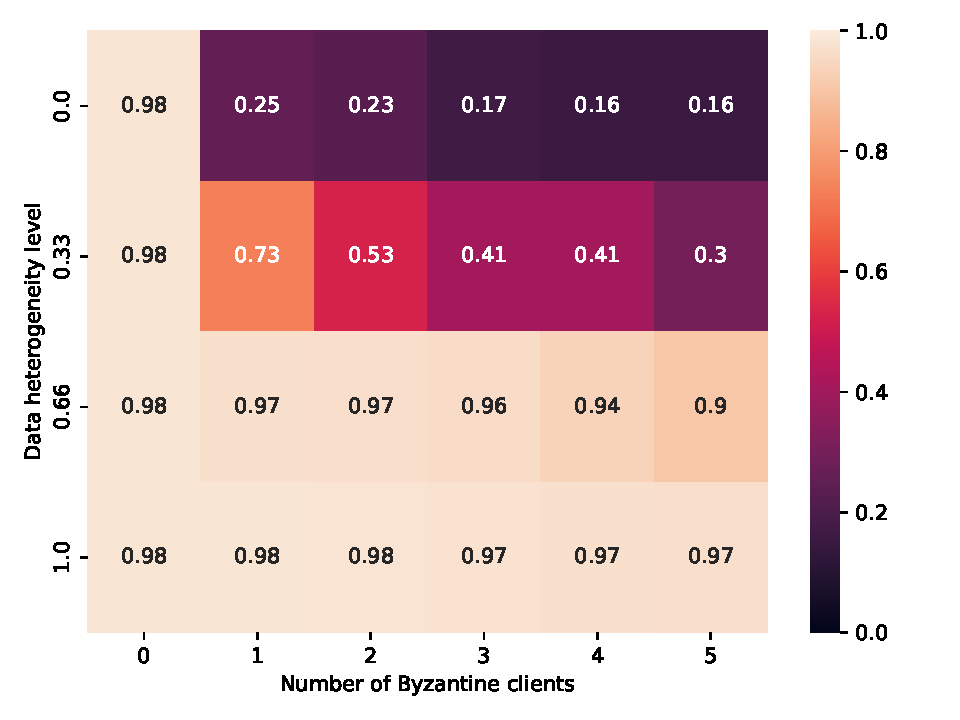
\includegraphics[width=\textwidth]{../plots/robust_comparison_sweep/best_test_mnist_cnn_mnist_gamma_similarity_niid_NNM_ARC_nb_honest_clients_10_tolerated_f_equal_real.pdf}
        \caption{CNN Baseline}
        \label{fig:best_overall_cnn}
    \end{subfigure}
    \hfill
    \begin{subfigure}[b]{0.24\textwidth}
        \centering
        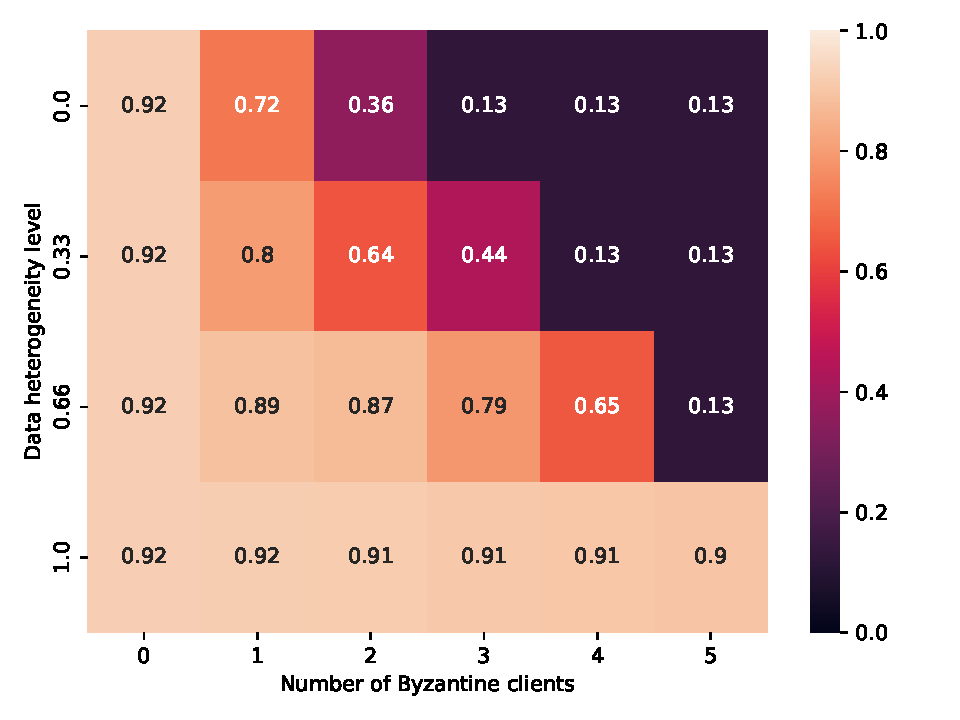
\includegraphics[width=\textwidth]{../plots/robust_new_atan_sweep/alpha_0.5/best_test_mnist_cnn_mnist_snn_gamma_similarity_niid_NNM_ARC_nb_honest_clients_10_tolerated_f_equal_real.pdf}
        \caption{$\alpha = 0.5$}
        \label{fig:best_overall_alpha_0_5}
    \end{subfigure}
    \hfill
    \begin{subfigure}[b]{0.24\textwidth}
        \centering
        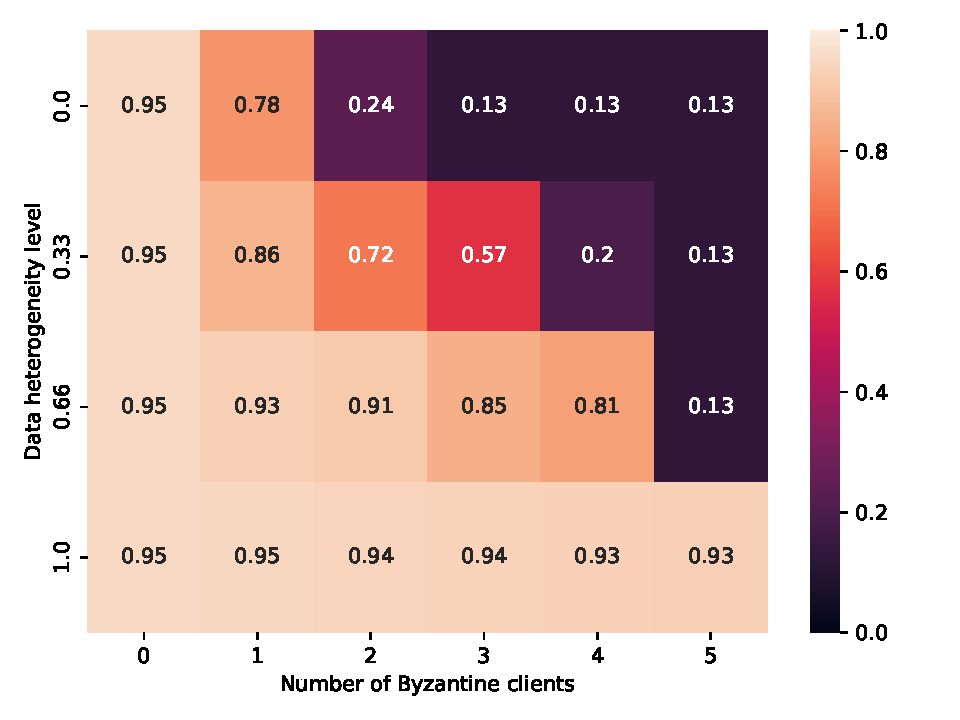
\includegraphics[width=\textwidth]{../plots/robust_new_atan_sweep/alpha_0.75/best_test_mnist_cnn_mnist_snn_gamma_similarity_niid_NNM_ARC_nb_honest_clients_10_tolerated_f_equal_real.pdf}
        \caption{$\alpha = 0.75$}
        \label{fig:best_overall_alpha_0_75}
    \end{subfigure}
    \hfill
    \begin{subfigure}[b]{0.24\textwidth}
        \centering
        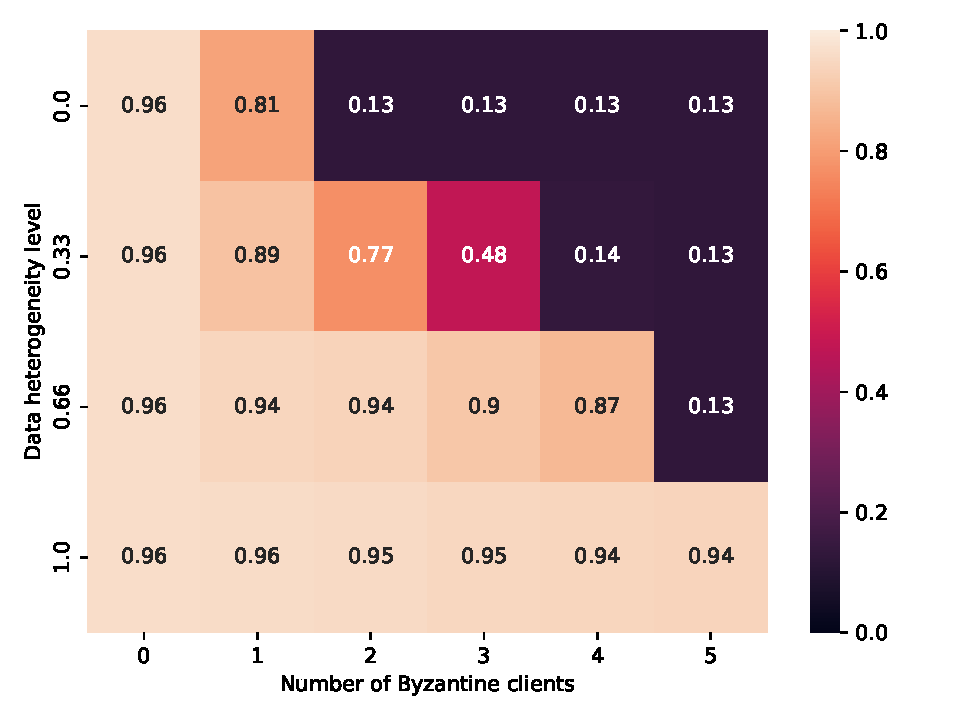
\includegraphics[width=\textwidth]{../plots/robust_new_atan_sweep/alpha_1.0/best_test_mnist_cnn_mnist_snn_gamma_similarity_niid_NNM_ARC_nb_honest_clients_10_tolerated_f_equal_real.pdf}
        \caption{$\alpha = 1.0$}
        \label{fig:best_overall_alpha_1_0}
    \end{subfigure}
    \vspace{0.2cm}
    \begin{subfigure}[b]{0.24\textwidth}
        \centering
        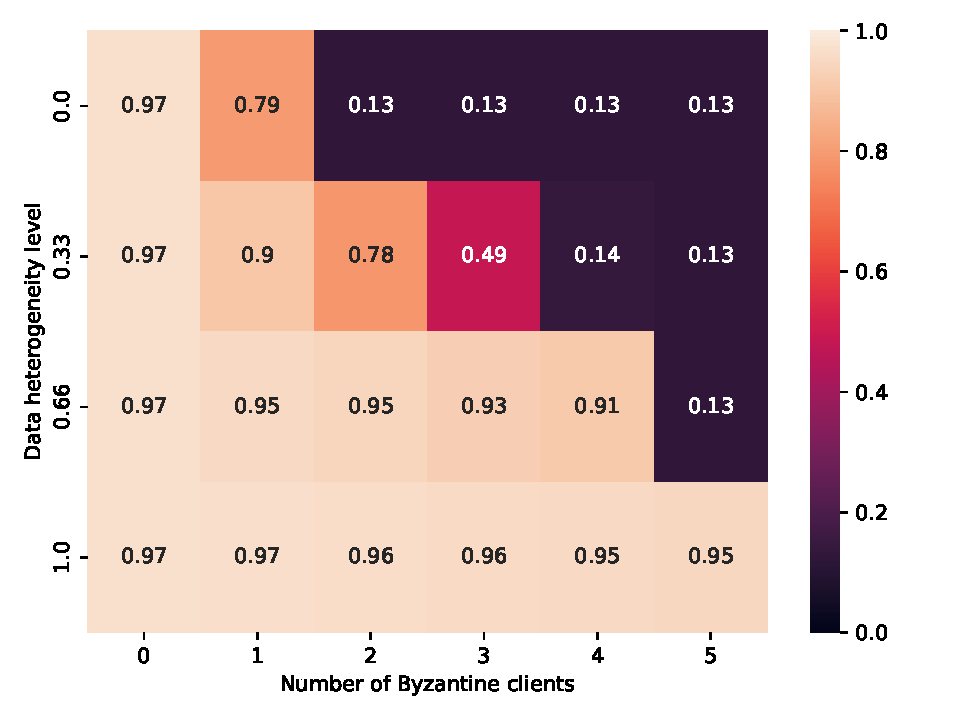
\includegraphics[width=\textwidth]{../plots/robust_new_atan_sweep/alpha_1.2/best_test_mnist_cnn_mnist_snn_gamma_similarity_niid_NNM_ARC_nb_honest_clients_10_tolerated_f_equal_real.pdf}
        \caption{$\alpha = 1.2$}
        \label{fig:best_overall_alpha_1_2}
    \end{subfigure}
    \hfill
    \begin{subfigure}[b]{0.24\textwidth}
        \centering
        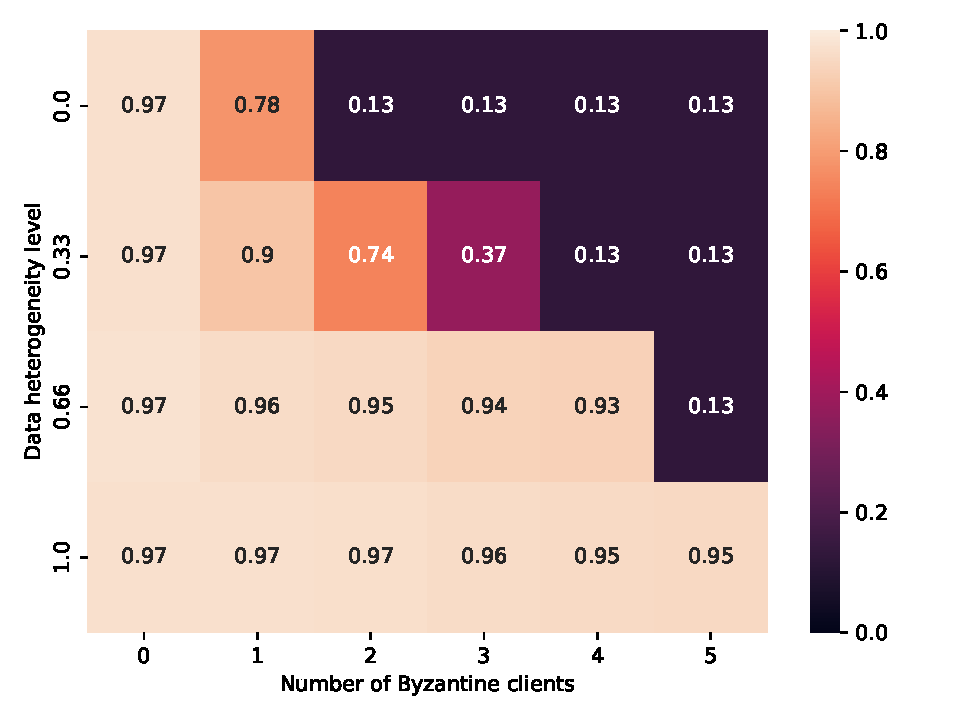
\includegraphics[width=\textwidth]{../plots/robust_new_atan_sweep/alpha_1.4/best_test_mnist_cnn_mnist_snn_gamma_similarity_niid_NNM_ARC_nb_honest_clients_10_tolerated_f_equal_real.pdf}
        \caption{$\alpha = 1.4$}
        \label{fig:best_overall_alpha_1_4}
    \end{subfigure}
    \hfill
    \begin{subfigure}[b]{0.24\textwidth}
        \centering
        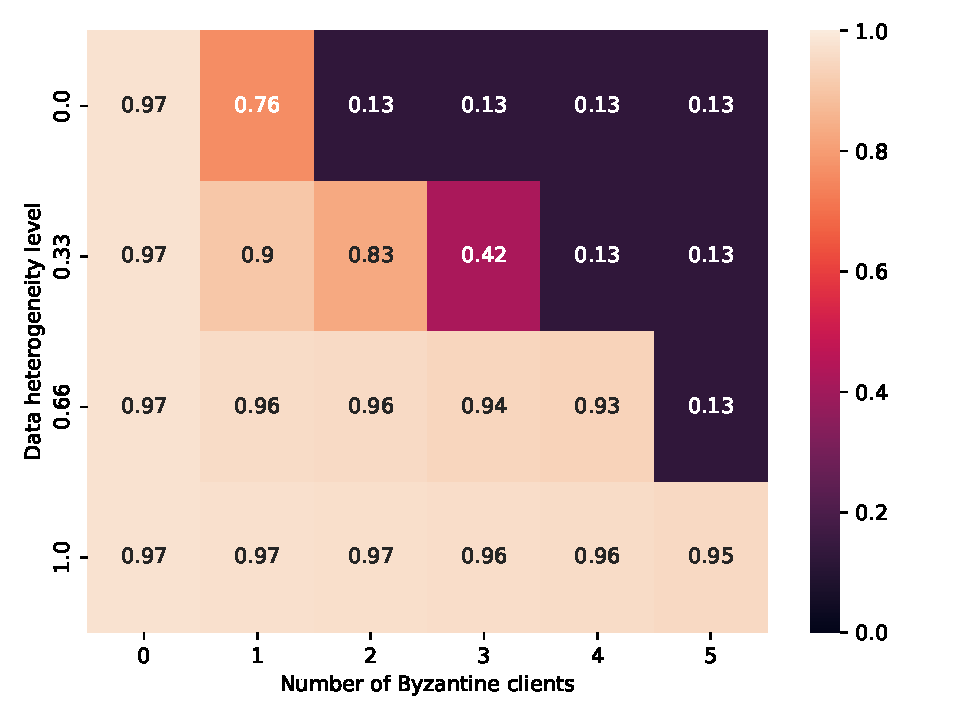
\includegraphics[width=\textwidth]{../plots/robust_new_atan_sweep/alpha_1.5/best_test_mnist_cnn_mnist_snn_gamma_similarity_niid_NNM_ARC_nb_honest_clients_10_tolerated_f_equal_real.pdf}
        \caption{$\alpha = 1.5$}
        \label{fig:best_overall_alpha_1_5}
    \end{subfigure}
    \hfill
    \begin{subfigure}[b]{0.24\textwidth}
        \centering
        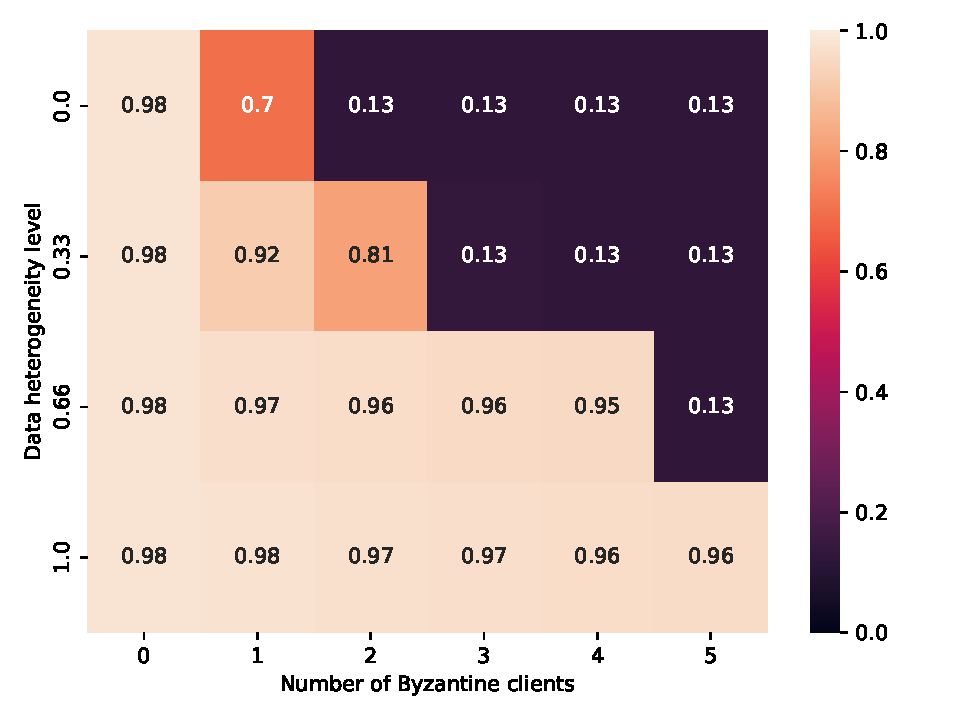
\includegraphics[width=\textwidth]{../plots/robust_new_atan_sweep/alpha_2.0/best_test_mnist_cnn_mnist_snn_gamma_similarity_niid_NNM_ARC_nb_honest_clients_10_tolerated_f_equal_real.pdf}
        \caption{$\alpha = 2.0$}
        \label{fig:best_overall_alpha_2_0}
    \end{subfigure}
    \caption{Best overall test accuracy heatmaps (worst-case across attacks) for different $\alpha$ stiffness parameter values.}
    \label{fig:best_overall_grid}
\end{figure}

\clearpage
\section{Best Aggregator under Specific Attacks}
This section presents heatmaps showing the best aggregator performance under each specific attack across all alphas.

\subsection{Optimal A Little Is Enough (ALIE) Attack}
\begin{figure}[htbp]
    \centering
    \begin{subfigure}[b]{0.24\textwidth}
        \centering
        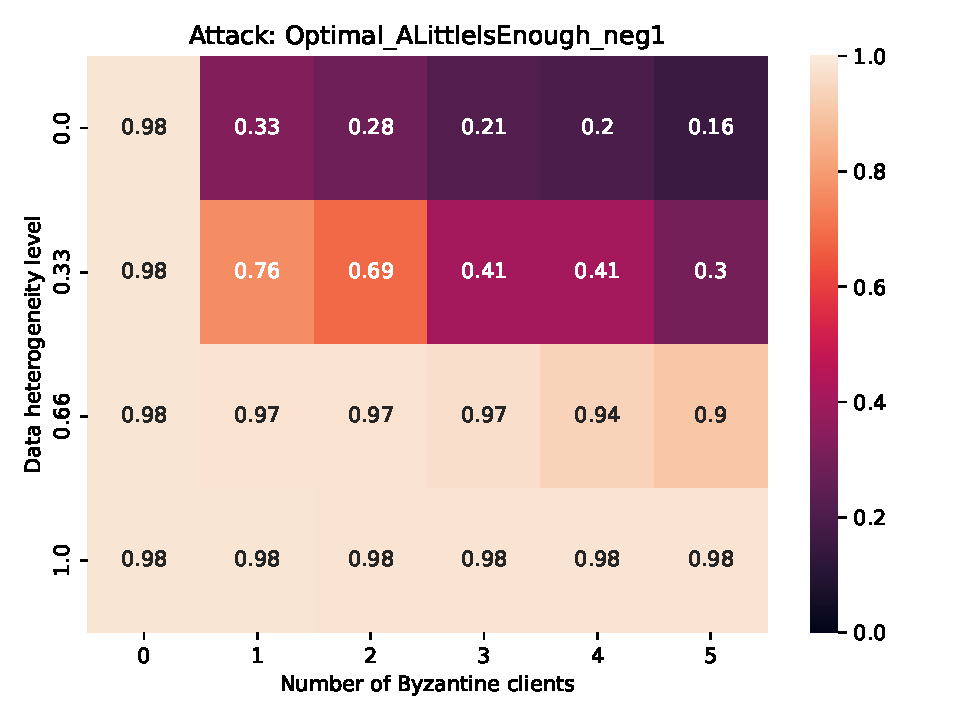
\includegraphics[width=\textwidth]{../plots/robust_comparison_sweep/best_test_Optimal_ALittleIsEnough_neg1_mnist_cnn_mnist_gamma_similarity_niid_NNM_ARC_nb_honest_clients_10_tolerated_f_equal_real.pdf}
        \caption{CNN Baseline}
        \label{fig:best_alie_cnn}
    \end{subfigure}
    \hfill
    \begin{subfigure}[b]{0.24\textwidth}
        \centering
        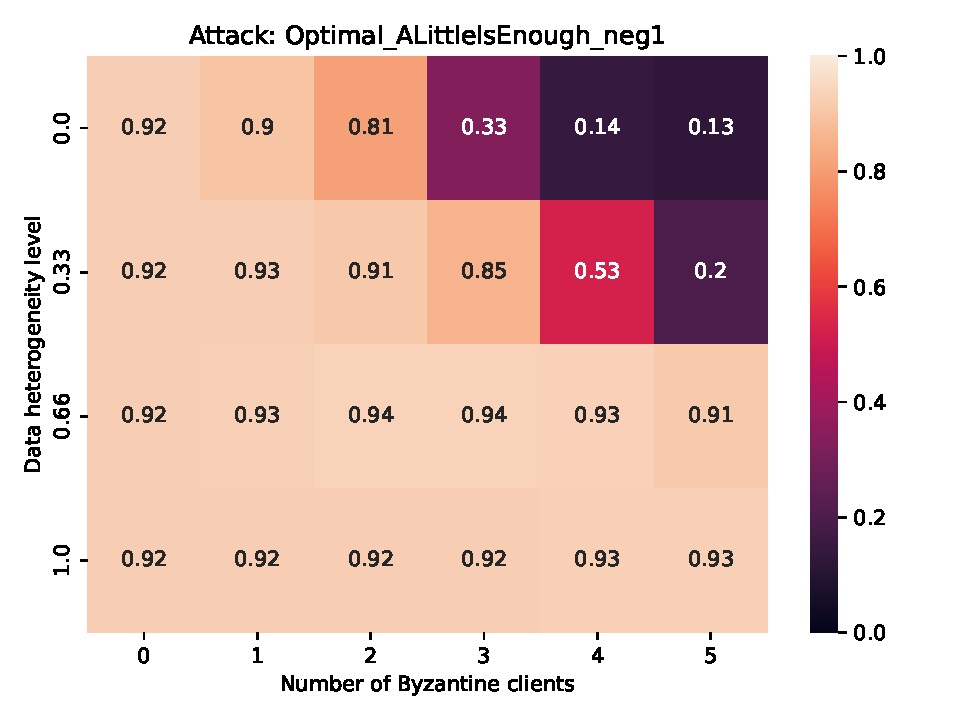
\includegraphics[width=\textwidth]{../plots/robust_new_atan_sweep/alpha_0.5/best_test_Optimal_ALittleIsEnough_neg1_mnist_cnn_mnist_snn_gamma_similarity_niid_NNM_ARC_nb_honest_clients_10_tolerated_f_equal_real.pdf}
        \caption{$\alpha = 0.5$}
        \label{fig:best_alie_alpha_0_5}
    \end{subfigure}
    \hfill
    \begin{subfigure}[b]{0.24\textwidth}
        \centering
        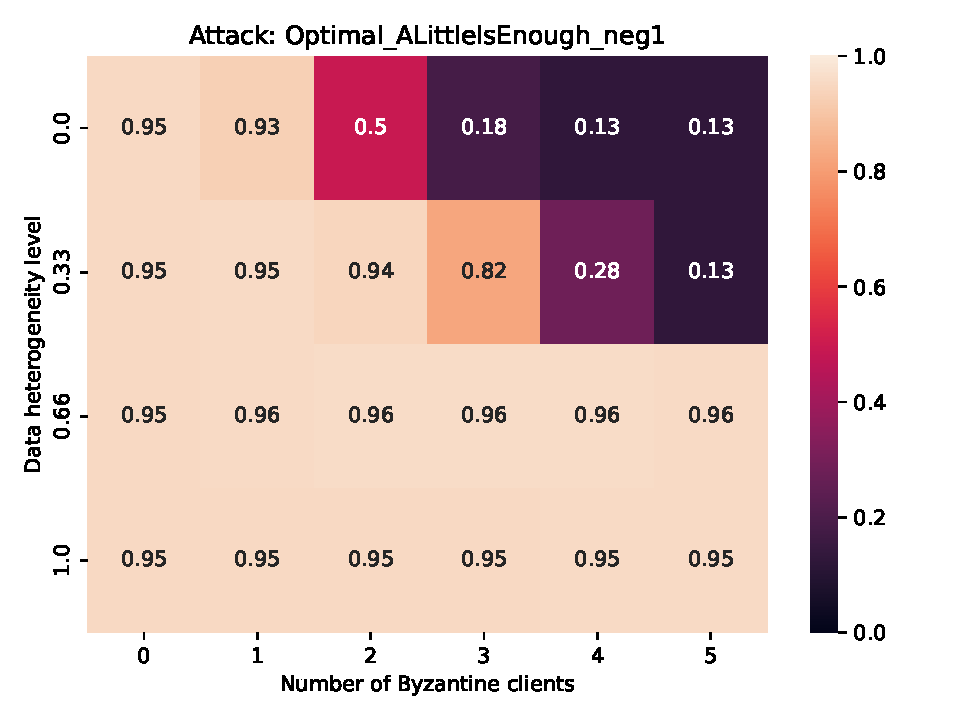
\includegraphics[width=\textwidth]{../plots/robust_new_atan_sweep/alpha_0.75/best_test_Optimal_ALittleIsEnough_neg1_mnist_cnn_mnist_snn_gamma_similarity_niid_NNM_ARC_nb_honest_clients_10_tolerated_f_equal_real.pdf}
        \caption{$\alpha = 0.75$}
        \label{fig:best_alie_alpha_0_75}
    \end{subfigure}
    \hfill
    \begin{subfigure}[b]{0.24\textwidth}
        \centering
        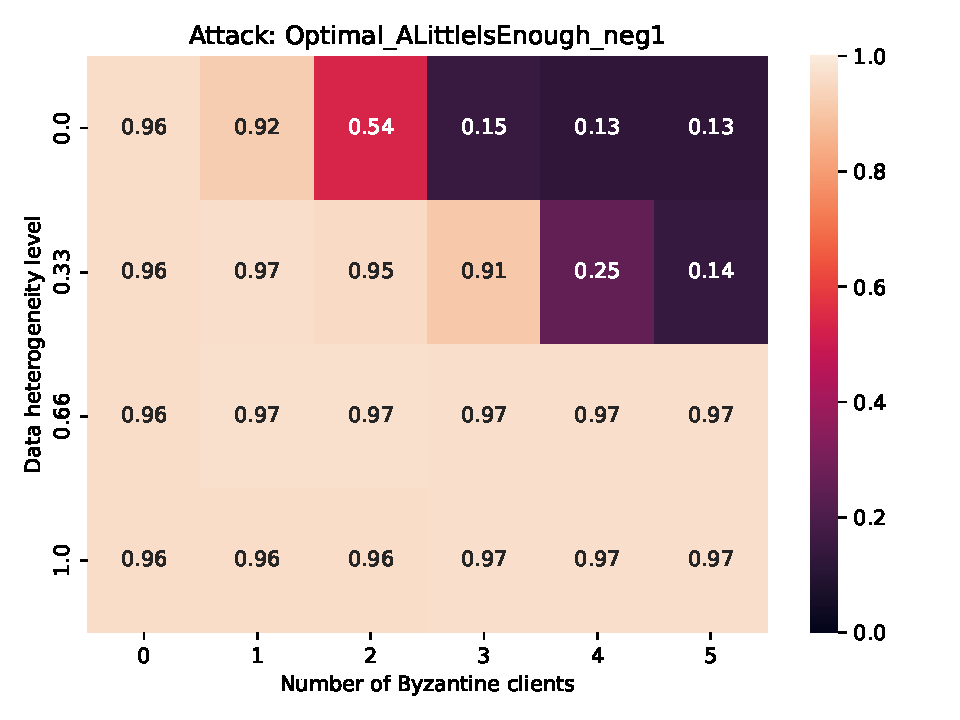
\includegraphics[width=\textwidth]{../plots/robust_new_atan_sweep/alpha_1.0/best_test_Optimal_ALittleIsEnough_neg1_mnist_cnn_mnist_snn_gamma_similarity_niid_NNM_ARC_nb_honest_clients_10_tolerated_f_equal_real.pdf}
        \caption{$\alpha = 1.0$}
        \label{fig:best_alie_alpha_1_0}
    \end{subfigure}
    \vspace{0.2cm}
    \begin{subfigure}[b]{0.24\textwidth}
        \centering
        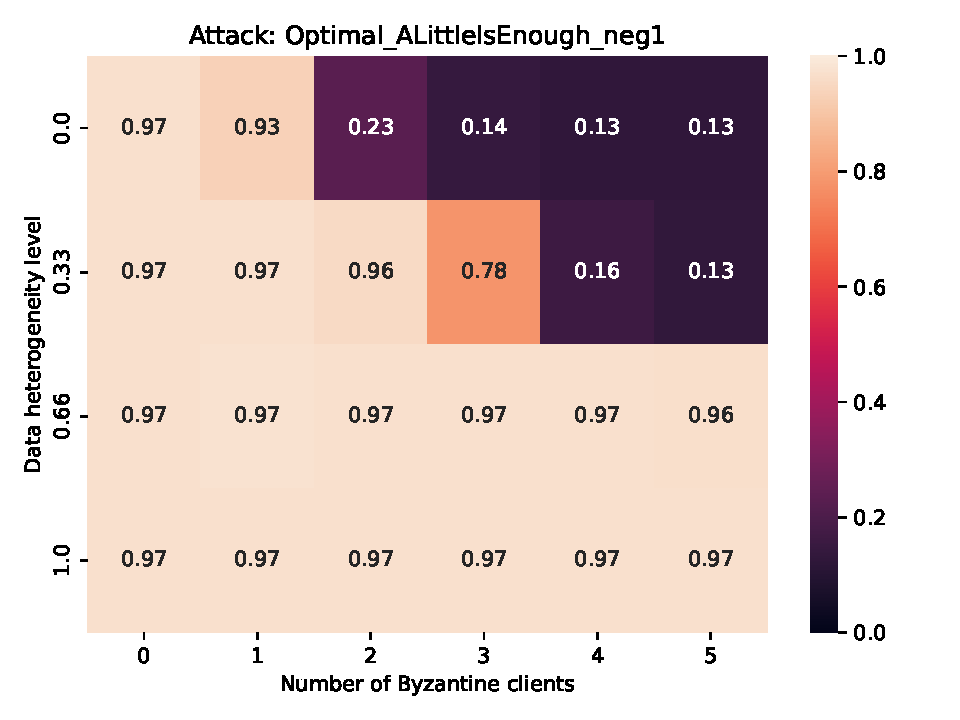
\includegraphics[width=\textwidth]{../plots/robust_new_atan_sweep/alpha_1.2/best_test_Optimal_ALittleIsEnough_neg1_mnist_cnn_mnist_snn_gamma_similarity_niid_NNM_ARC_nb_honest_clients_10_tolerated_f_equal_real.pdf}
        \caption{$\alpha = 1.2$}
        \label{fig:best_alie_alpha_1_2}
    \end{subfigure}
    \hfill
    \begin{subfigure}[b]{0.24\textwidth}
        \centering
        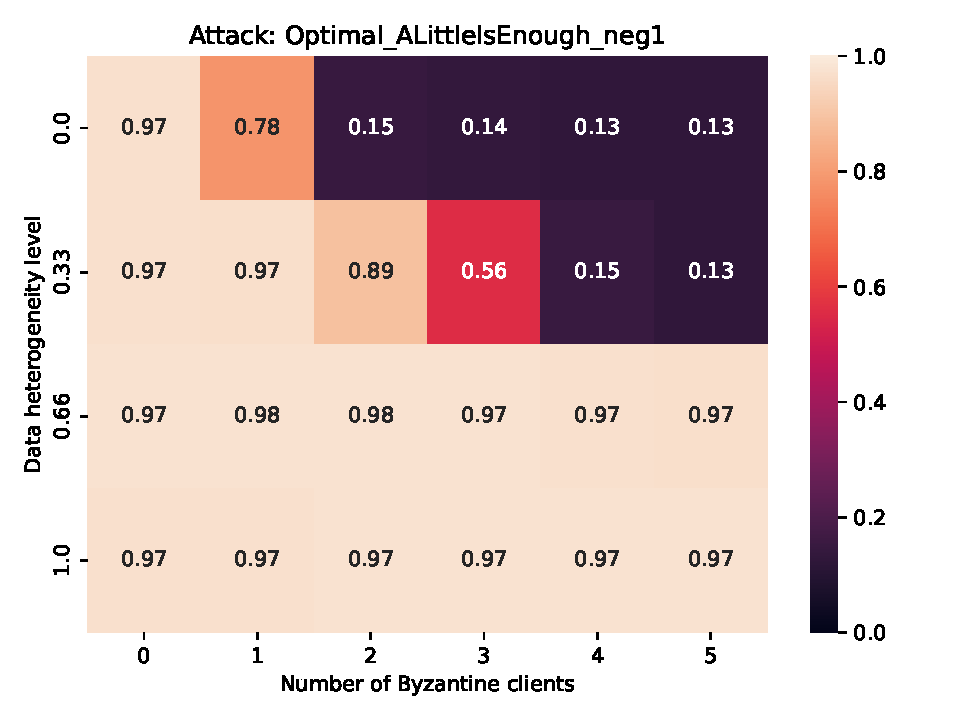
\includegraphics[width=\textwidth]{../plots/robust_new_atan_sweep/alpha_1.4/best_test_Optimal_ALittleIsEnough_neg1_mnist_cnn_mnist_snn_gamma_similarity_niid_NNM_ARC_nb_honest_clients_10_tolerated_f_equal_real.pdf}
        \caption{$\alpha = 1.4$}
        \label{fig:best_alie_alpha_1_4}
    \end{subfigure}
    \hfill
    \begin{subfigure}[b]{0.24\textwidth}
        \centering
        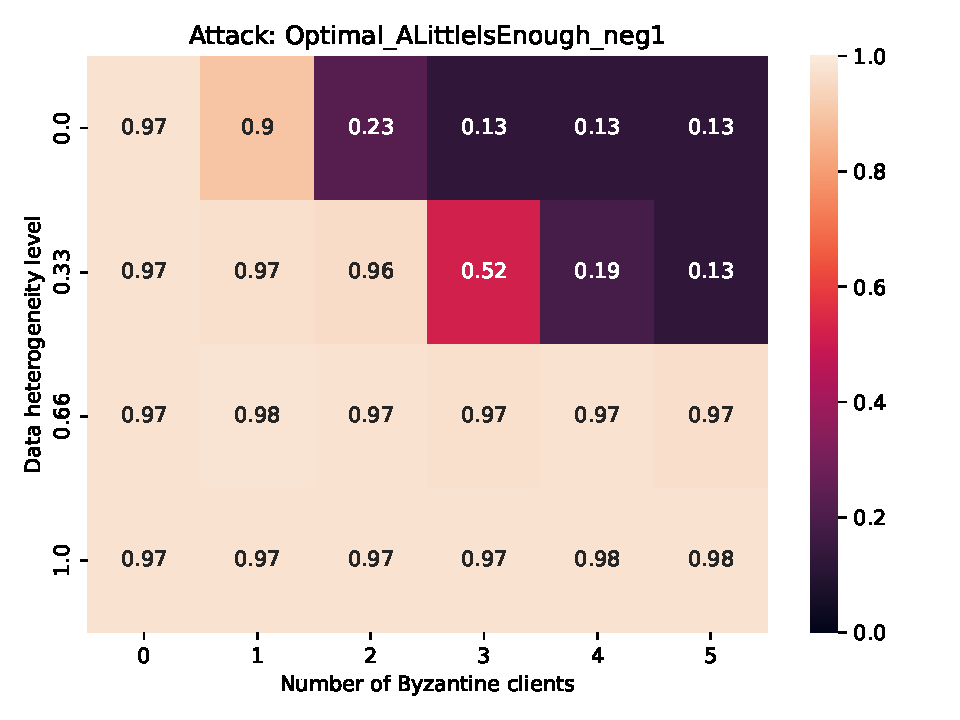
\includegraphics[width=\textwidth]{../plots/robust_new_atan_sweep/alpha_1.5/best_test_Optimal_ALittleIsEnough_neg1_mnist_cnn_mnist_snn_gamma_similarity_niid_NNM_ARC_nb_honest_clients_10_tolerated_f_equal_real.pdf}
        \caption{$\alpha = 1.5$}
        \label{fig:best_alie_alpha_1_5}
    \end{subfigure}
    \hfill
    \begin{subfigure}[b]{0.24\textwidth}
        \centering
        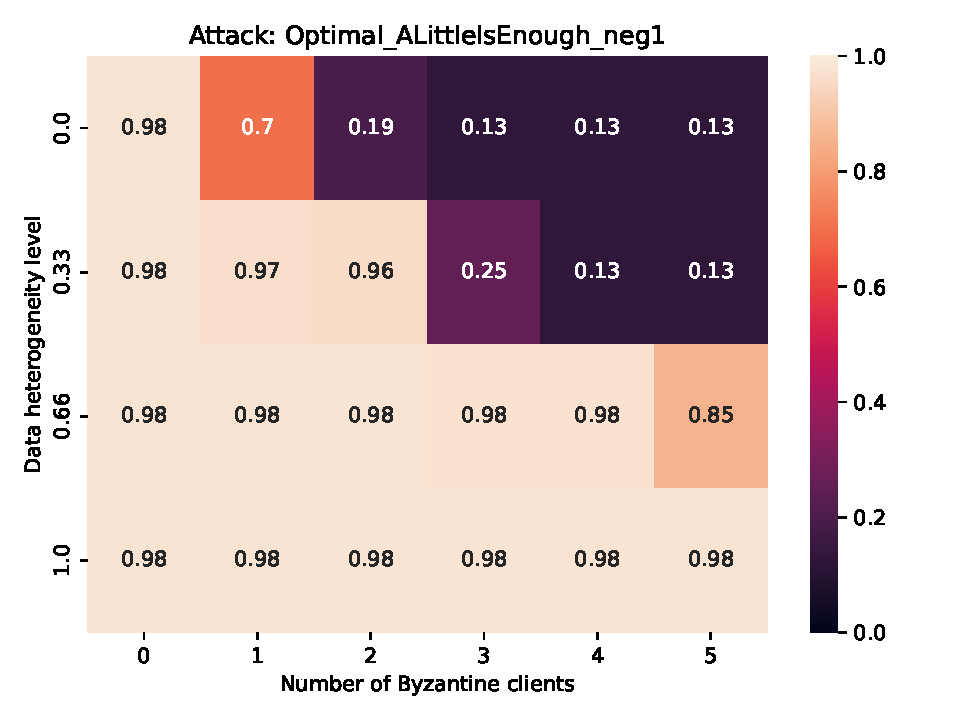
\includegraphics[width=\textwidth]{../plots/robust_new_atan_sweep/alpha_2.0/best_test_Optimal_ALittleIsEnough_neg1_mnist_cnn_mnist_snn_gamma_similarity_niid_NNM_ARC_nb_honest_clients_10_tolerated_f_equal_real.pdf}
        \caption{$\alpha = 2.0$}
        \label{fig:best_alie_alpha_2_0}
    \end{subfigure}
    \caption{Best test accuracy heatmaps under the Optimal ALIE attack for different $\alpha$ parameter values.}
    \label{fig:best_alie_grid}
\end{figure}
\clearpage
\subsection{Sign Flipping Attack}
\begin{figure}[htbp]
    \centering
    \begin{subfigure}[b]{0.24\textwidth}
        \centering
        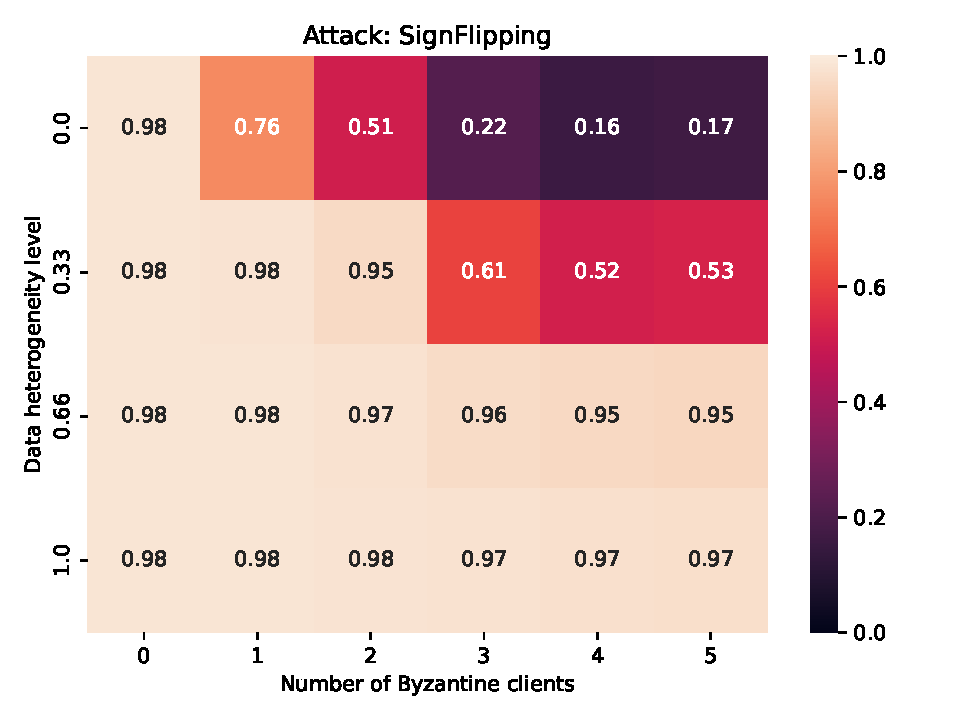
\includegraphics[width=\textwidth]{../plots/robust_comparison_sweep/best_test_SignFlipping_mnist_cnn_mnist_gamma_similarity_niid_NNM_ARC_nb_honest_clients_10_tolerated_f_equal_real.pdf}
        \caption{CNN Baseline}
        \label{fig:best_sf_cnn}
    \end{subfigure}
    \hfill
    \begin{subfigure}[b]{0.24\textwidth}
        \centering
        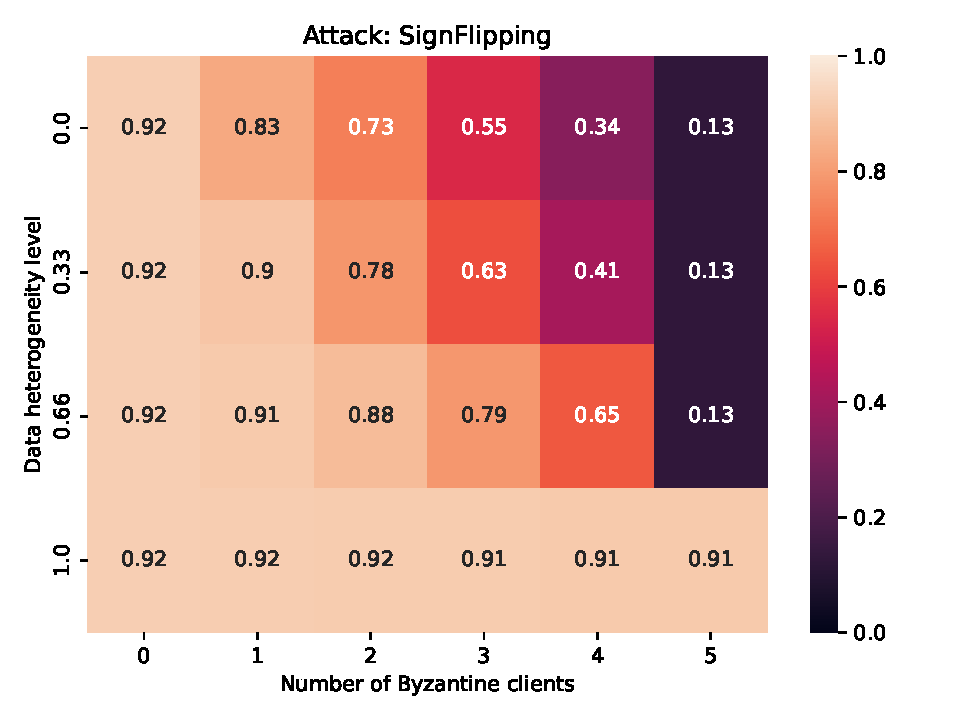
\includegraphics[width=\textwidth]{../plots/robust_new_atan_sweep/alpha_0.5/best_test_SignFlipping_mnist_cnn_mnist_snn_gamma_similarity_niid_NNM_ARC_nb_honest_clients_10_tolerated_f_equal_real.pdf}
        \caption{$\alpha = 0.5$}
        \label{fig:best_sf_alpha_0_5}
    \end{subfigure}
    \hfill
    \begin{subfigure}[b]{0.24\textwidth}
        \centering
        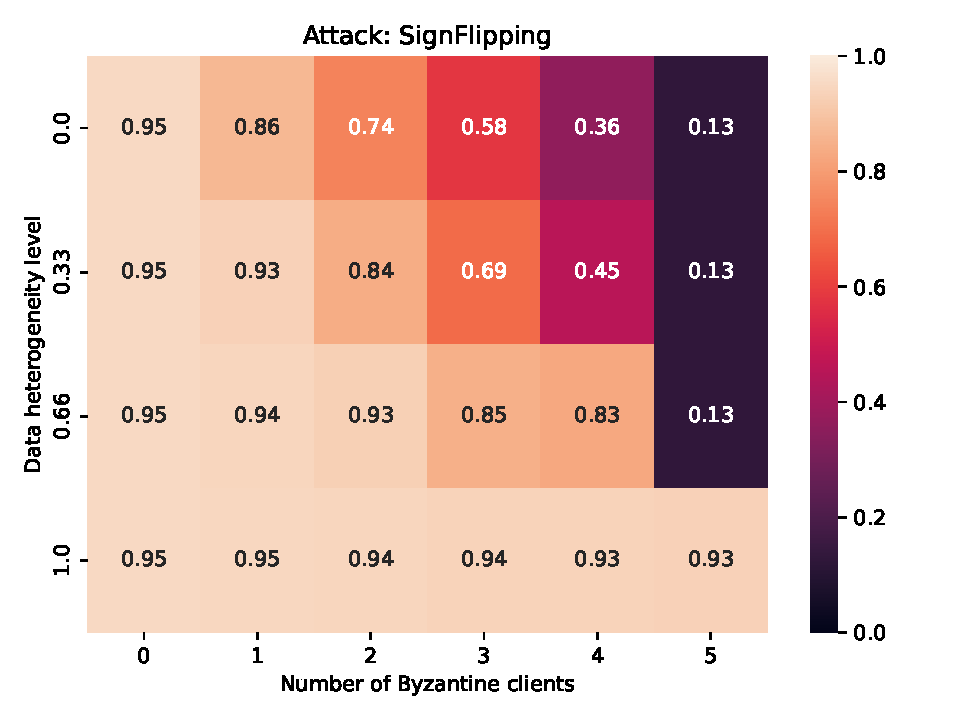
\includegraphics[width=\textwidth]{../plots/robust_new_atan_sweep/alpha_0.75/best_test_SignFlipping_mnist_cnn_mnist_snn_gamma_similarity_niid_NNM_ARC_nb_honest_clients_10_tolerated_f_equal_real.pdf}
        \caption{$\alpha = 0.75$}
        \label{fig:best_sf_alpha_0_75}
    \end{subfigure}
    \hfill
    \begin{subfigure}[b]{0.24\textwidth}
        \centering
        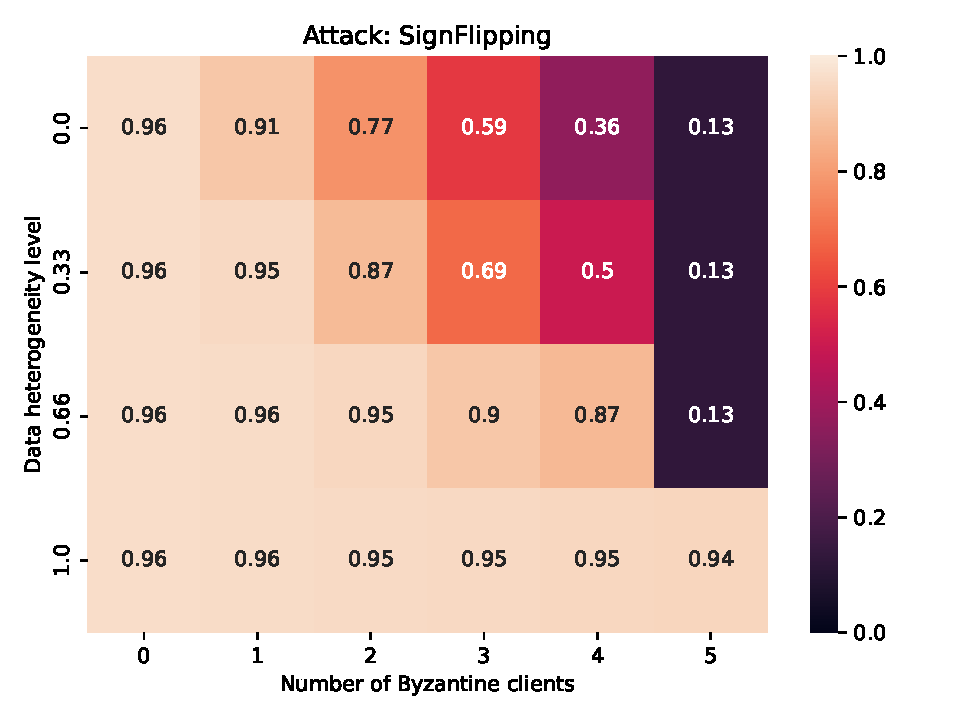
\includegraphics[width=\textwidth]{../plots/robust_new_atan_sweep/alpha_1.0/best_test_SignFlipping_mnist_cnn_mnist_snn_gamma_similarity_niid_NNM_ARC_nb_honest_clients_10_tolerated_f_equal_real.pdf}
        \caption{$\alpha = 1.0$}
        \label{fig:best_sf_alpha_1_0}
    \end{subfigure}
    \vspace{0.2cm}
    \begin{subfigure}[b]{0.24\textwidth}
        \centering
        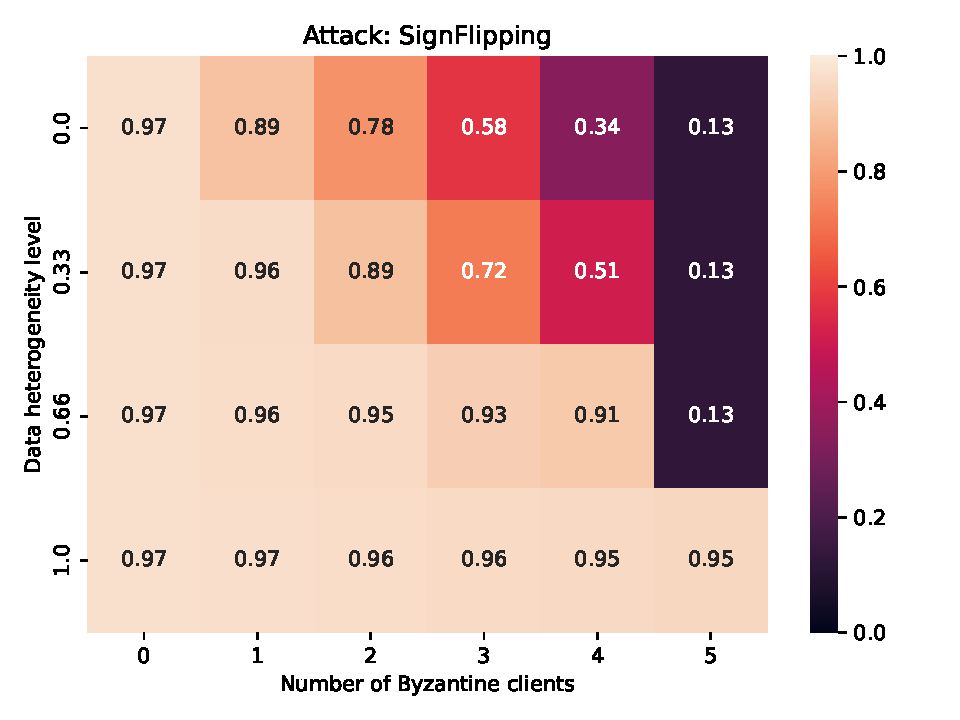
\includegraphics[width=\textwidth]{../plots/robust_new_atan_sweep/alpha_1.2/best_test_SignFlipping_mnist_cnn_mnist_snn_gamma_similarity_niid_NNM_ARC_nb_honest_clients_10_tolerated_f_equal_real.pdf}
        \caption{$\alpha = 1.2$}
        \label{fig:best_sf_alpha_1_2}
    \end{subfigure}
    \hfill
    \begin{subfigure}[b]{0.24\textwidth}
        \centering
        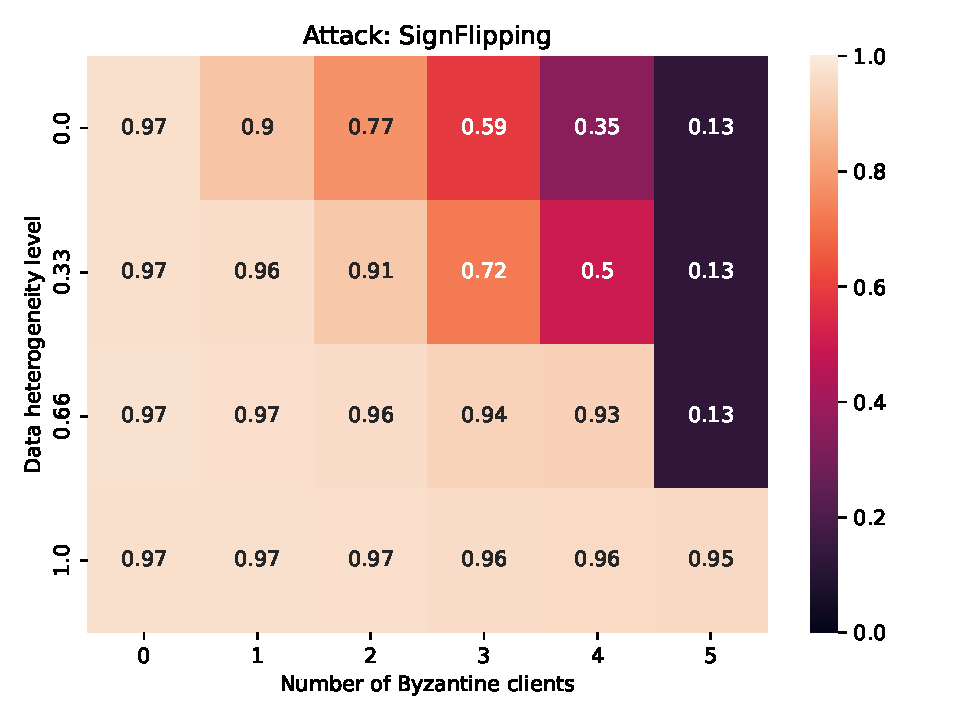
\includegraphics[width=\textwidth]{../plots/robust_new_atan_sweep/alpha_1.4/best_test_SignFlipping_mnist_cnn_mnist_snn_gamma_similarity_niid_NNM_ARC_nb_honest_clients_10_tolerated_f_equal_real.pdf}
        \caption{$\alpha = 1.4$}
        \label{fig:best_sf_alpha_1_4}
    \end{subfigure}
    \hfill
    \begin{subfigure}[b]{0.24\textwidth}
        \centering
        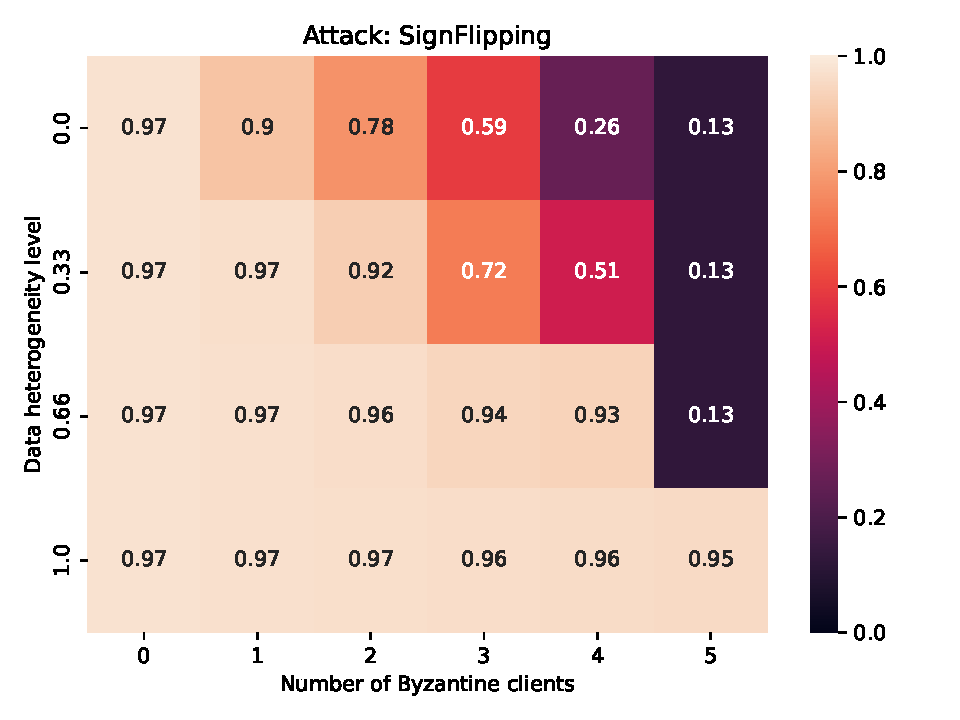
\includegraphics[width=\textwidth]{../plots/robust_new_atan_sweep/alpha_1.5/best_test_SignFlipping_mnist_cnn_mnist_snn_gamma_similarity_niid_NNM_ARC_nb_honest_clients_10_tolerated_f_equal_real.pdf}
        \caption{$\alpha = 1.5$}
        \label{fig:best_sf_alpha_1_5}
    \end{subfigure}
    \hfill
    \begin{subfigure}[b]{0.24\textwidth}
        \centering
        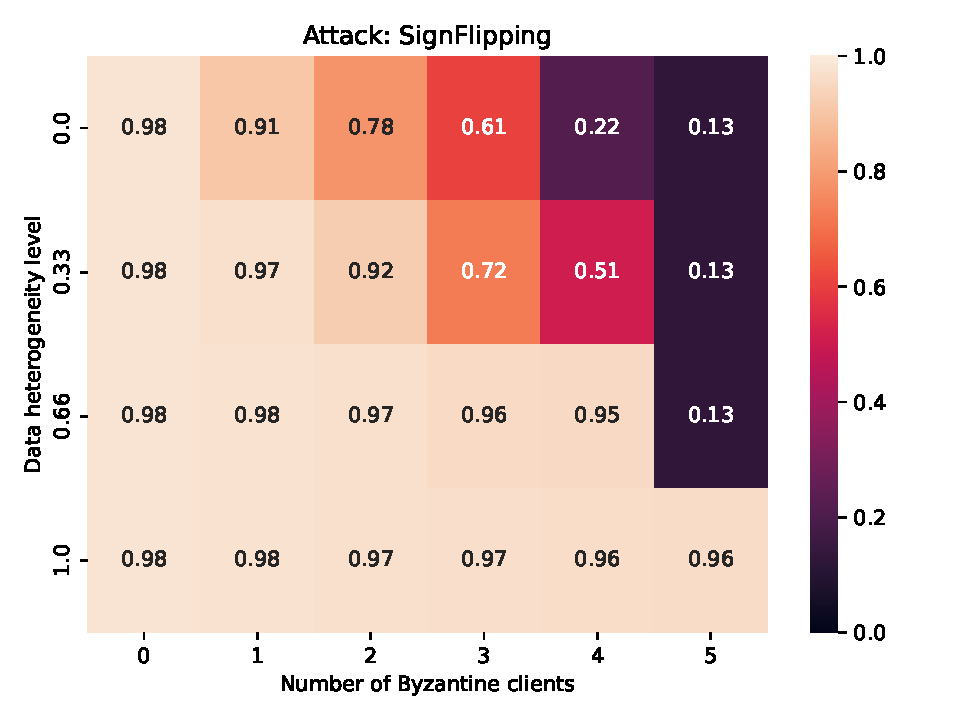
\includegraphics[width=\textwidth]{../plots/robust_new_atan_sweep/alpha_2.0/best_test_SignFlipping_mnist_cnn_mnist_snn_gamma_similarity_niid_NNM_ARC_nb_honest_clients_10_tolerated_f_equal_real.pdf}
        \caption{$\alpha = 2.0$}
        \label{fig:best_sf_alpha_2_0}
    \end{subfigure}
    \caption{Best test accuracy heatmaps under the Sign Flipping attack for different $\alpha$ parameter values.}
    \label{fig:best_sf_grid}
\end{figure}
\clearpage
\subsection{Optimal Inner Product Manipulation Attack}
\begin{figure}[htbp]
    \centering
    \begin{subfigure}[b]{0.24\textwidth}
        \centering
        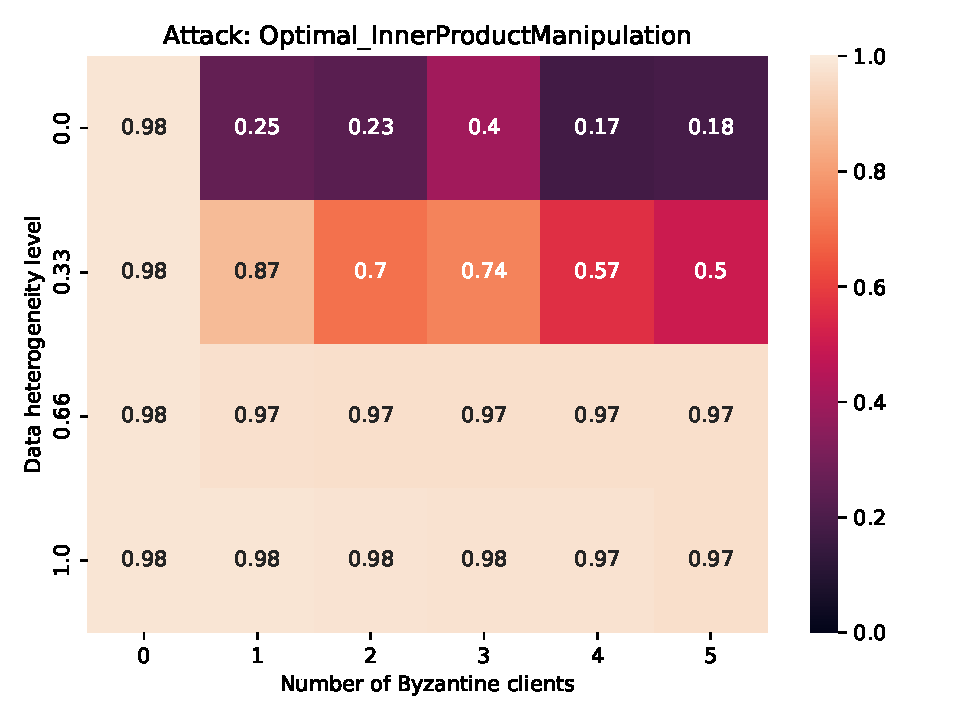
\includegraphics[width=\textwidth]{../plots/robust_comparison_sweep/best_test_Optimal_InnerProductManipulation_mnist_cnn_mnist_gamma_similarity_niid_NNM_ARC_nb_honest_clients_10_tolerated_f_equal_real.pdf}
        \caption{CNN Baseline}
        \label{fig:best_ipm_cnn}
    \end{subfigure}
    \hfill
    \begin{subfigure}[b]{0.24\textwidth}
        \centering
        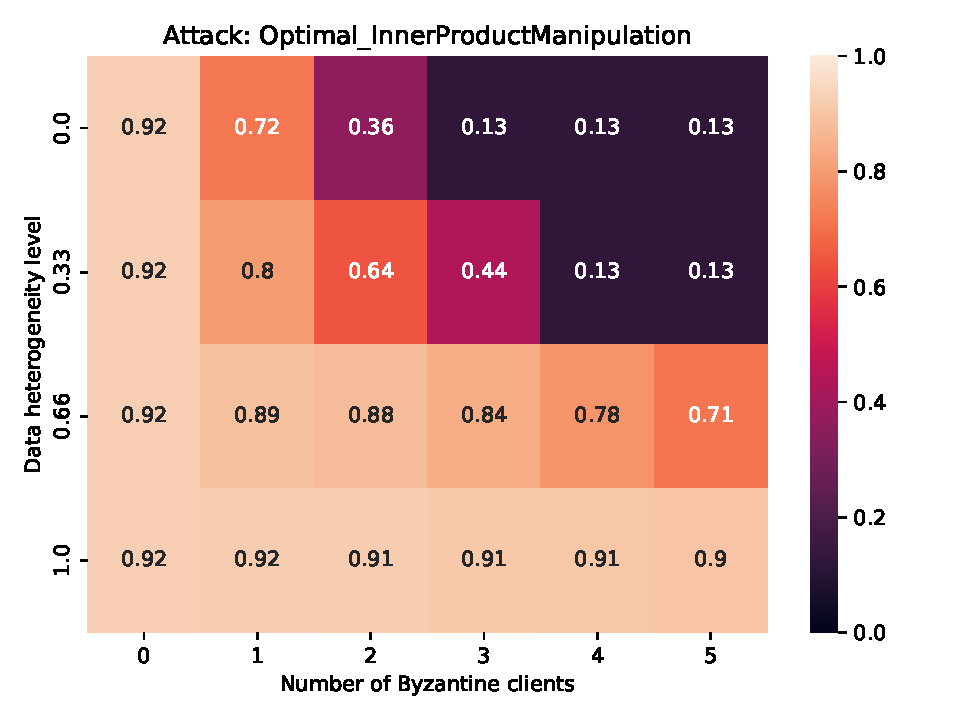
\includegraphics[width=\textwidth]{../plots/robust_new_atan_sweep/alpha_0.5/best_test_Optimal_InnerProductManipulation_mnist_cnn_mnist_snn_gamma_similarity_niid_NNM_ARC_nb_honest_clients_10_tolerated_f_equal_real.pdf}
        \caption{$\alpha = 0.5$}
        \label{fig:best_ipm_alpha_0_5}
    \end{subfigure}
    \hfill
    \begin{subfigure}[b]{0.24\textwidth}
        \centering
        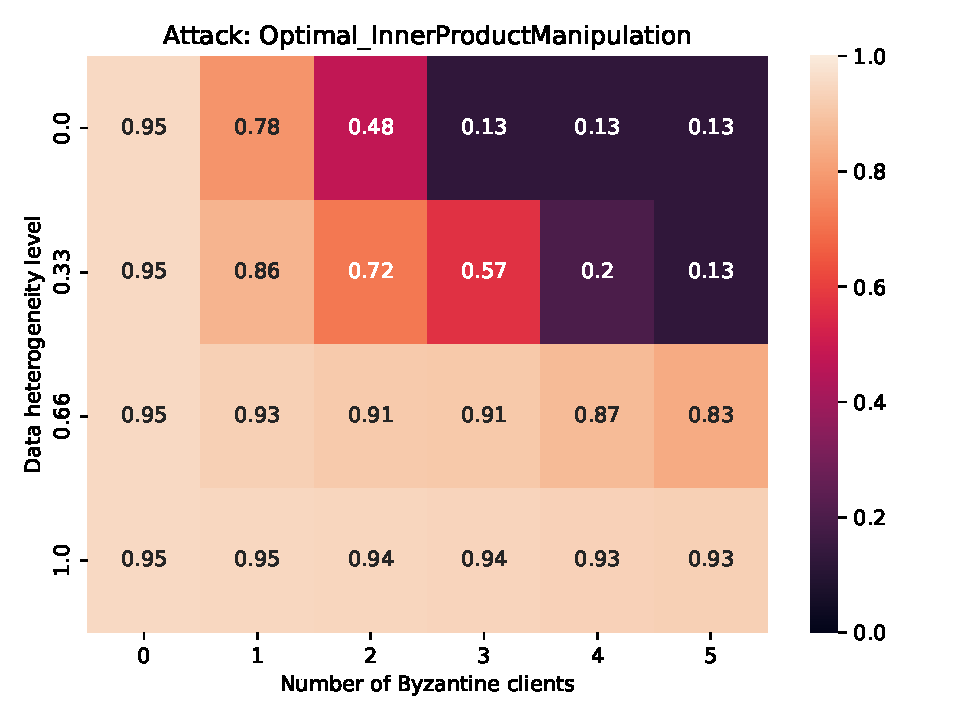
\includegraphics[width=\textwidth]{../plots/robust_new_atan_sweep/alpha_0.75/best_test_Optimal_InnerProductManipulation_mnist_cnn_mnist_snn_gamma_similarity_niid_NNM_ARC_nb_honest_clients_10_tolerated_f_equal_real.pdf}
        \caption{$\alpha = 0.75$}
        \label{fig:best_ipm_alpha_0_75}
    \end{subfigure}
    \hfill
    \begin{subfigure}[b]{0.24\textwidth}
        \centering
        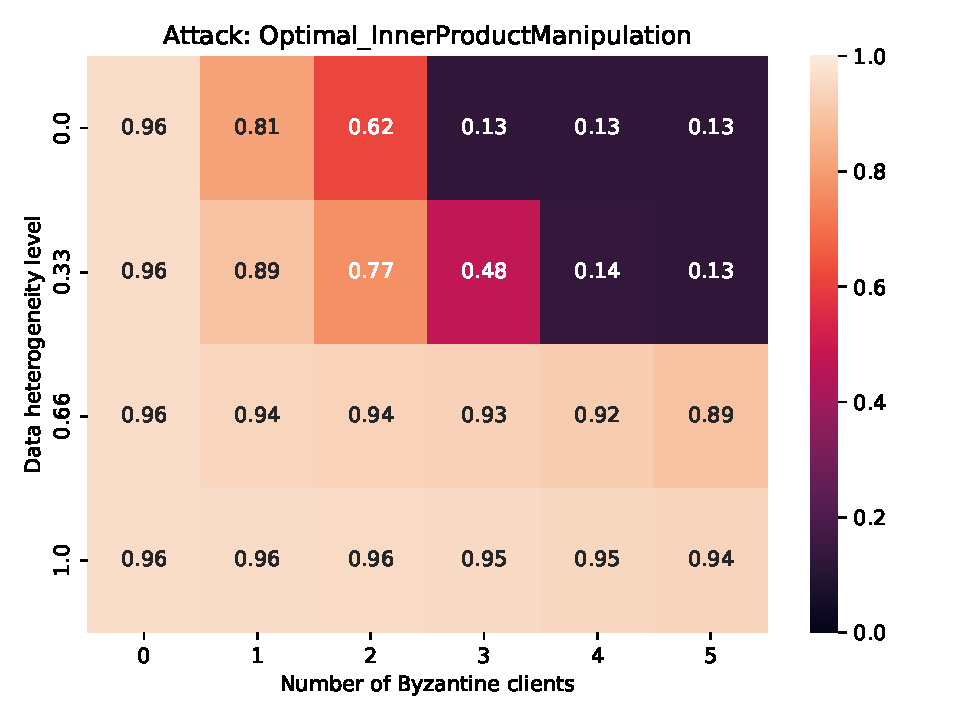
\includegraphics[width=\textwidth]{../plots/robust_new_atan_sweep/alpha_1.0/best_test_Optimal_InnerProductManipulation_mnist_cnn_mnist_snn_gamma_similarity_niid_NNM_ARC_nb_honest_clients_10_tolerated_f_equal_real.pdf}
        \caption{$\alpha = 1.0$}
        \label{fig:best_ipm_alpha_1_0}
    \end{subfigure}
    \vspace{0.2cm}
    \begin{subfigure}[b]{0.24\textwidth}
        \centering
        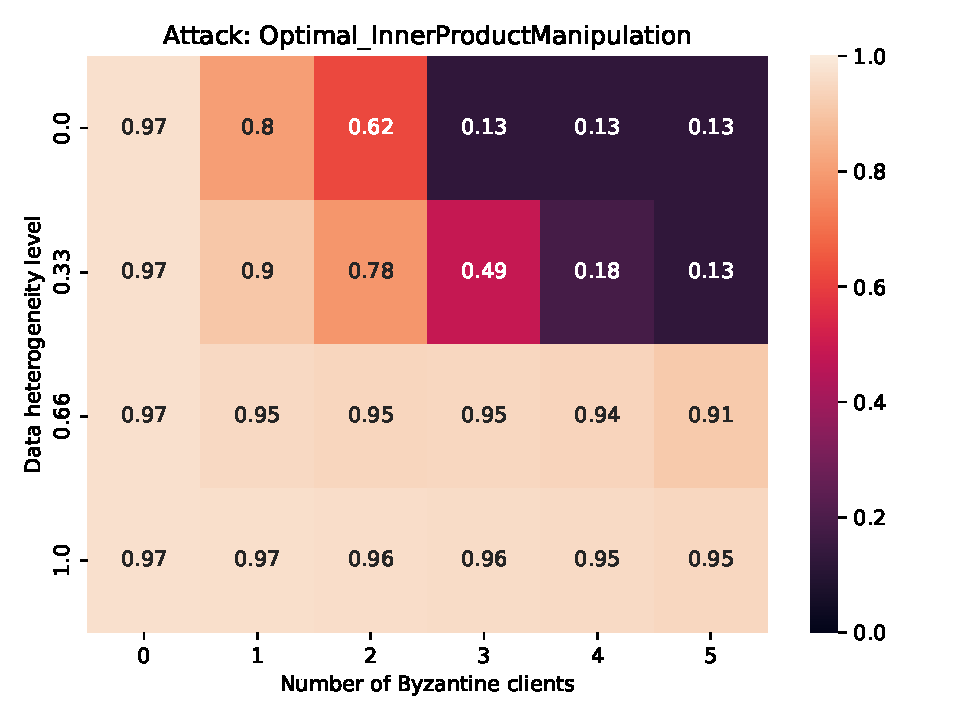
\includegraphics[width=\textwidth]{../plots/robust_new_atan_sweep/alpha_1.2/best_test_Optimal_InnerProductManipulation_mnist_cnn_mnist_snn_gamma_similarity_niid_NNM_ARC_nb_honest_clients_10_tolerated_f_equal_real.pdf}
        \caption{$\alpha = 1.2$}
        \label{fig:best_ipm_alpha_1_2}
    \end{subfigure}
    \hfill
    \begin{subfigure}[b]{0.24\textwidth}
        \centering
        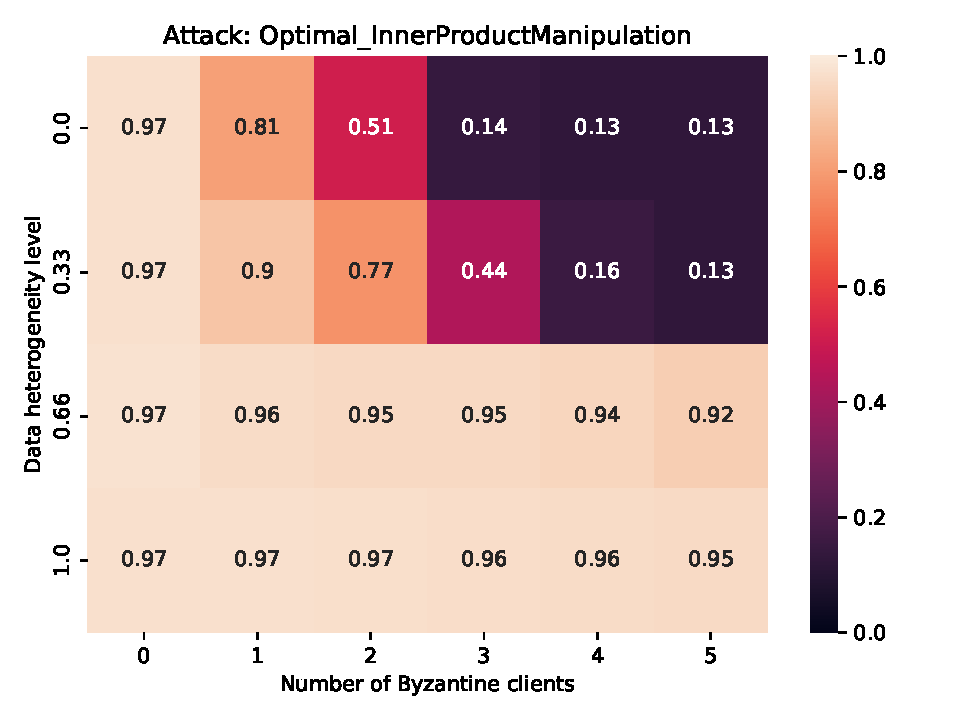
\includegraphics[width=\textwidth]{../plots/robust_new_atan_sweep/alpha_1.4/best_test_Optimal_InnerProductManipulation_mnist_cnn_mnist_snn_gamma_similarity_niid_NNM_ARC_nb_honest_clients_10_tolerated_f_equal_real.pdf}
        \caption{$\alpha = 1.4$}
        \label{fig:best_ipm_alpha_1_4}
    \end{subfigure}
    \hfill
    \begin{subfigure}[b]{0.24\textwidth}
        \centering
        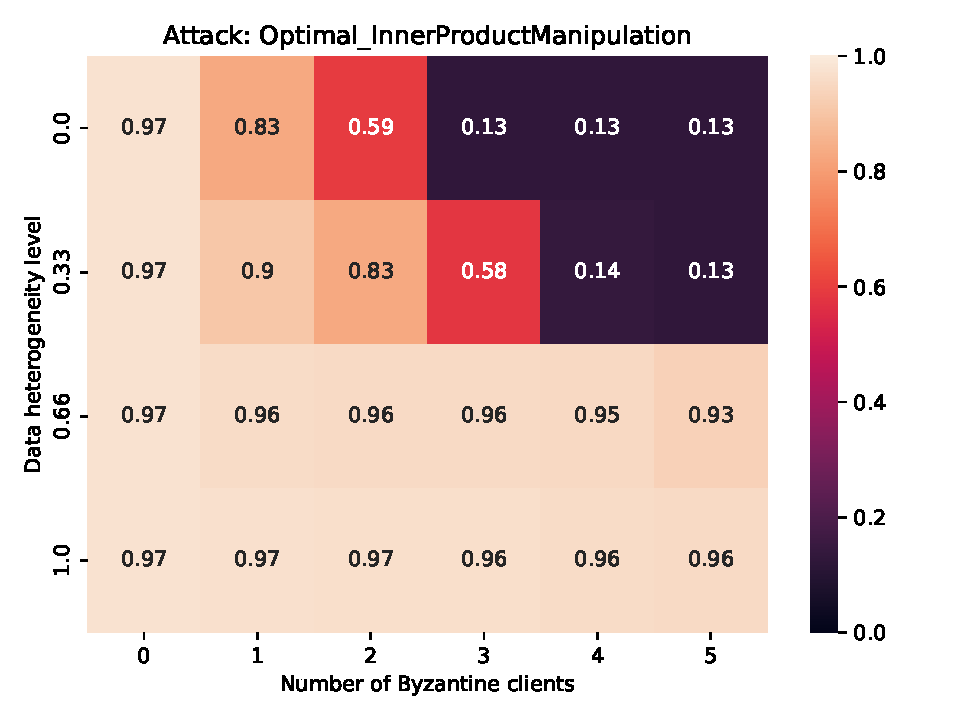
\includegraphics[width=\textwidth]{../plots/robust_new_atan_sweep/alpha_1.5/best_test_Optimal_InnerProductManipulation_mnist_cnn_mnist_snn_gamma_similarity_niid_NNM_ARC_nb_honest_clients_10_tolerated_f_equal_real.pdf}
        \caption{$\alpha = 1.5$}
        \label{fig:best_ipm_alpha_1_5}
    \end{subfigure}
    \hfill
    \begin{subfigure}[b]{0.24\textwidth}
        \centering
        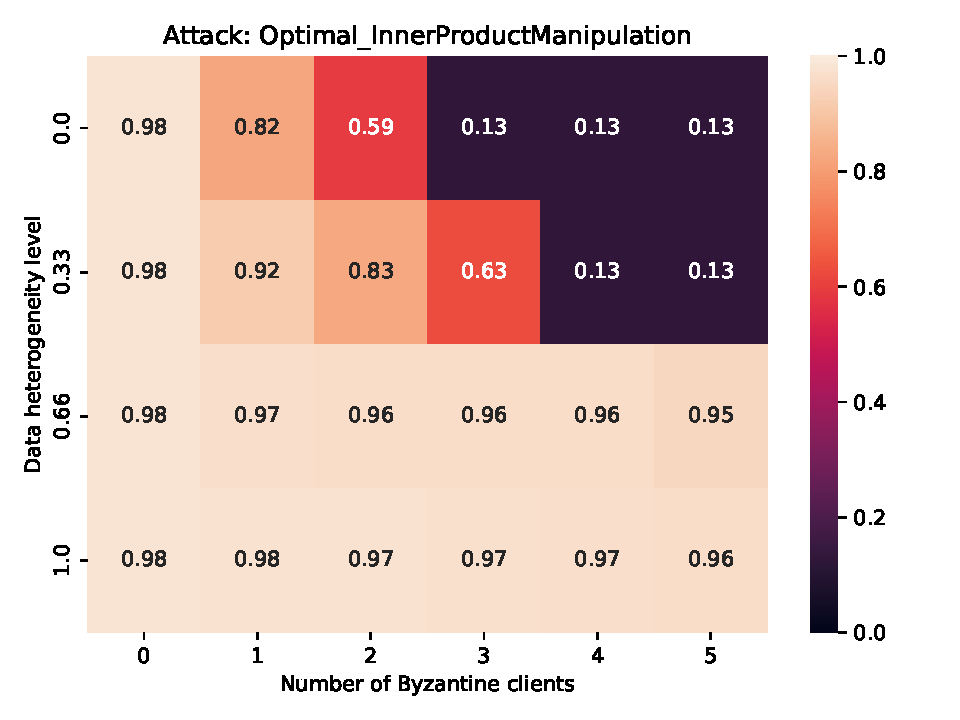
\includegraphics[width=\textwidth]{../plots/robust_new_atan_sweep/alpha_2.0/best_test_Optimal_InnerProductManipulation_mnist_cnn_mnist_snn_gamma_similarity_niid_NNM_ARC_nb_honest_clients_10_tolerated_f_equal_real.pdf}
        \caption{$\alpha = 2.0$}
        \label{fig:best_ipm_alpha_2_0}
    \end{subfigure}
    \caption{Best test accuracy heatmaps under the Optimal Inner Product Manipulation attack for different $\alpha$ parameter values.}
    \label{fig:best_ipm_grid}
\end{figure}

\clearpage
\section{Robustness of Fixed Aggregators across all Attacks}
In this section, we analyze the performance of each specific aggregator (Centered Clipping, Geometric Median, Multi-Krum, Trimmed Mean) across all Byzantine attack settings for different stiffness $\alpha$ values.

\clearpage
\subsection{Centered Clipping (CC)}
\subsubsection{CC under Worst-Case across all Attacks}
\begin{figure}[htbp]
    \centering
    \begin{subfigure}[b]{0.24\textwidth}
        \centering
        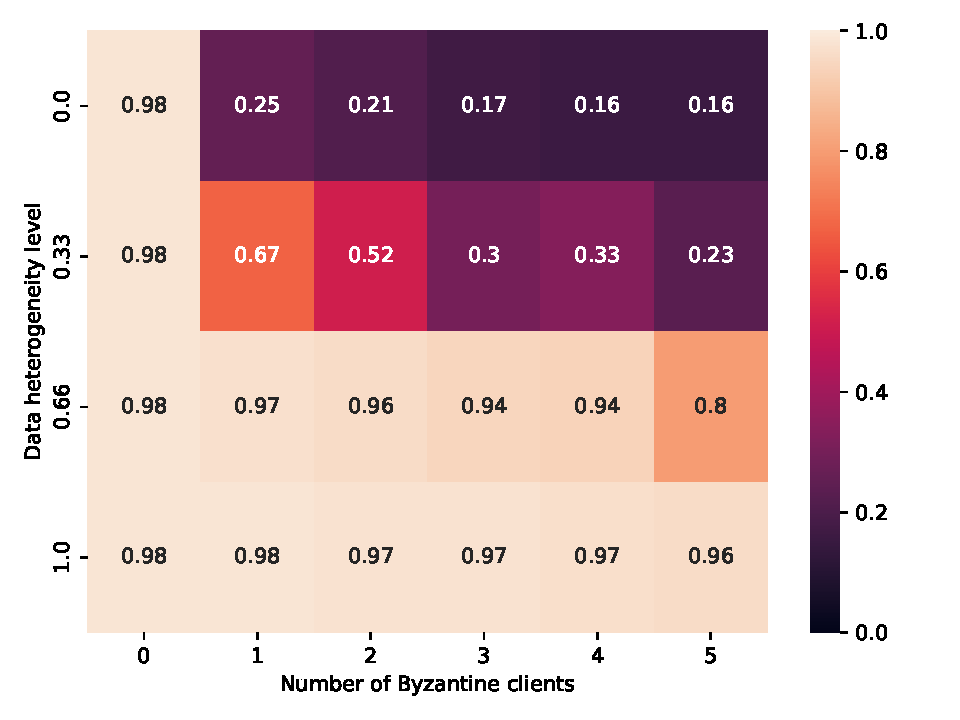
\includegraphics[width=\textwidth]{../plots/robust_comparison_sweep/test_mnist_cnn_mnist_gamma_similarity_niid_NNM_ARC_CenteredClipping_nb_honest_clients_10_tolerated_f_equal_real.pdf}
        \caption{CNN Baseline}
        \label{fig:cc_worst_case_cnn}
    \end{subfigure}
    \hfill
    \begin{subfigure}[b]{0.24\textwidth}
        \centering
        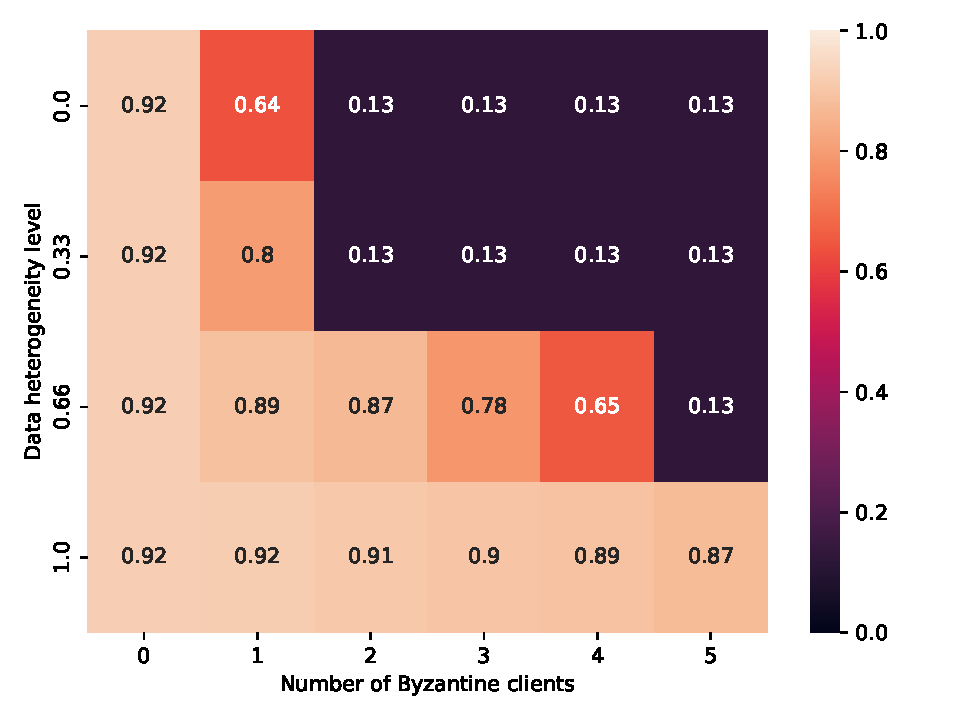
\includegraphics[width=\textwidth]{../plots/robust_new_atan_sweep/alpha_0.5/test_mnist_cnn_mnist_snn_gamma_similarity_niid_NNM_ARC_CenteredClipping_nb_honest_clients_10_tolerated_f_equal_real.pdf}
        \caption{$\alpha = 0.5$}
        \label{fig:cc_worst_case_alpha_0_5}
    \end{subfigure}
    \hfill
    \begin{subfigure}[b]{0.24\textwidth}
        \centering
        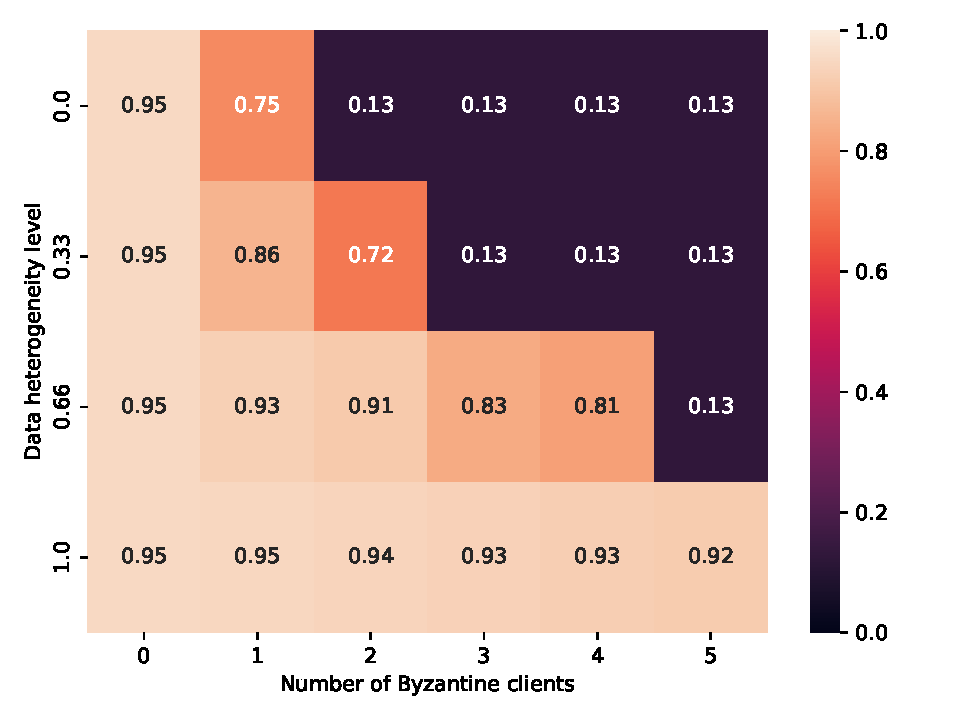
\includegraphics[width=\textwidth]{../plots/robust_new_atan_sweep/alpha_0.75/test_mnist_cnn_mnist_snn_gamma_similarity_niid_NNM_ARC_CenteredClipping_nb_honest_clients_10_tolerated_f_equal_real.pdf}
        \caption{$\alpha = 0.75$}
        \label{fig:cc_worst_case_alpha_0_75}
    \end{subfigure}
    \hfill
    \begin{subfigure}[b]{0.24\textwidth}
        \centering
        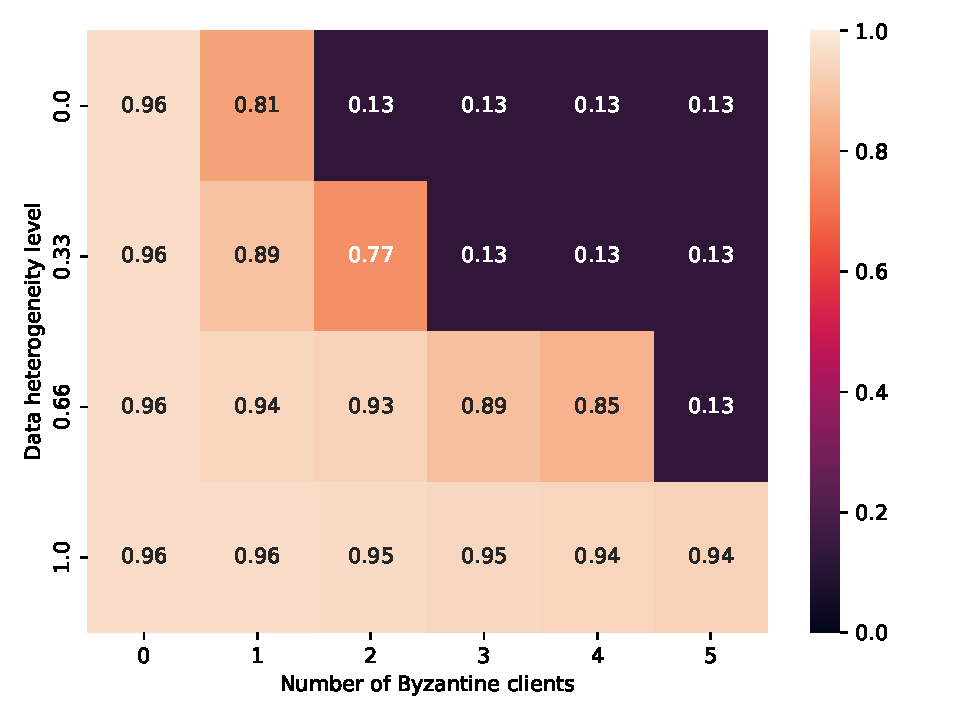
\includegraphics[width=\textwidth]{../plots/robust_new_atan_sweep/alpha_1.0/test_mnist_cnn_mnist_snn_gamma_similarity_niid_NNM_ARC_CenteredClipping_nb_honest_clients_10_tolerated_f_equal_real.pdf}
        \caption{$\alpha = 1.0$}
        \label{fig:cc_worst_case_alpha_1_0}
    \end{subfigure}
    \vspace{0.2cm}
    \begin{subfigure}[b]{0.24\textwidth}
        \centering
        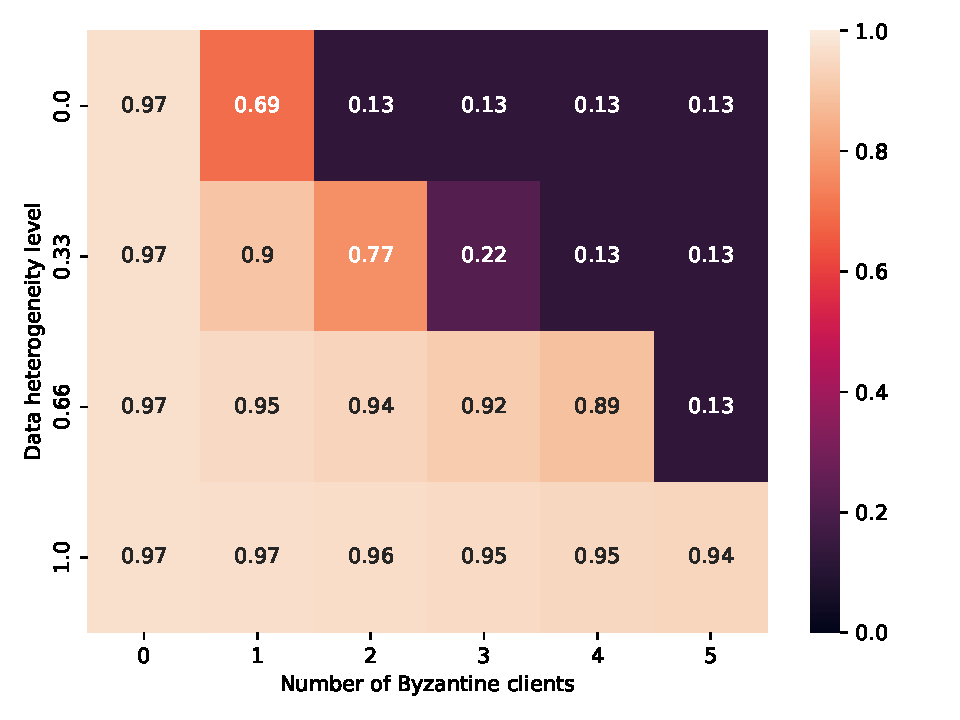
\includegraphics[width=\textwidth]{../plots/robust_new_atan_sweep/alpha_1.2/test_mnist_cnn_mnist_snn_gamma_similarity_niid_NNM_ARC_CenteredClipping_nb_honest_clients_10_tolerated_f_equal_real.pdf}
        \caption{$\alpha = 1.2$}
        \label{fig:cc_worst_case_alpha_1_2}
    \end{subfigure}
    \hfill
    \begin{subfigure}[b]{0.24\textwidth}
        \centering
        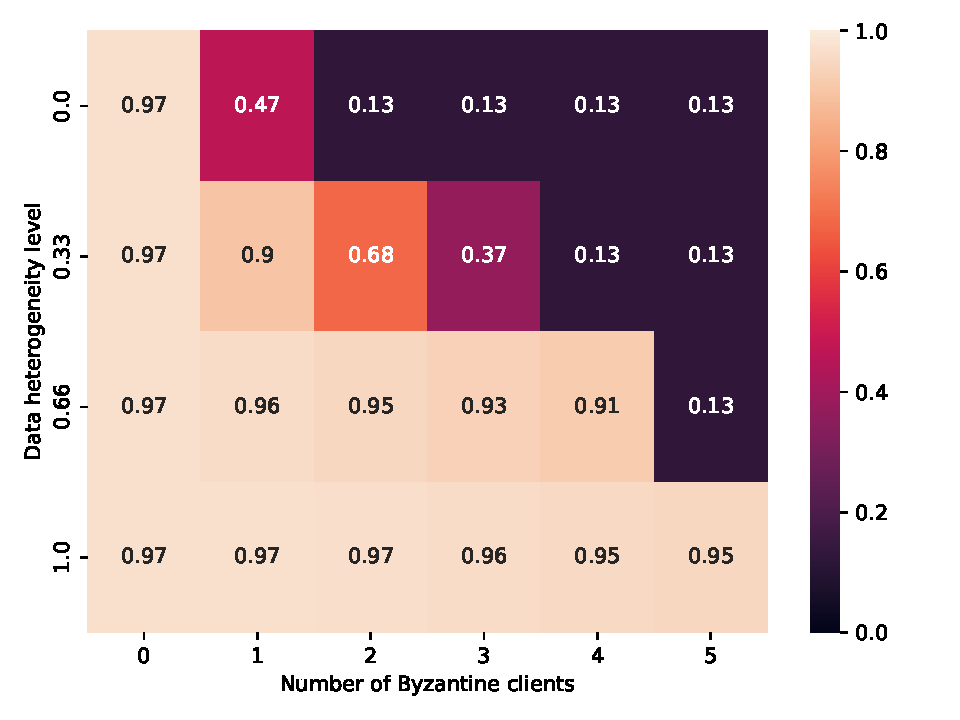
\includegraphics[width=\textwidth]{../plots/robust_new_atan_sweep/alpha_1.4/test_mnist_cnn_mnist_snn_gamma_similarity_niid_NNM_ARC_CenteredClipping_nb_honest_clients_10_tolerated_f_equal_real.pdf}
        \caption{$\alpha = 1.4$}
        \label{fig:cc_worst_case_alpha_1_4}
    \end{subfigure}
    \hfill
    \begin{subfigure}[b]{0.24\textwidth}
        \centering
        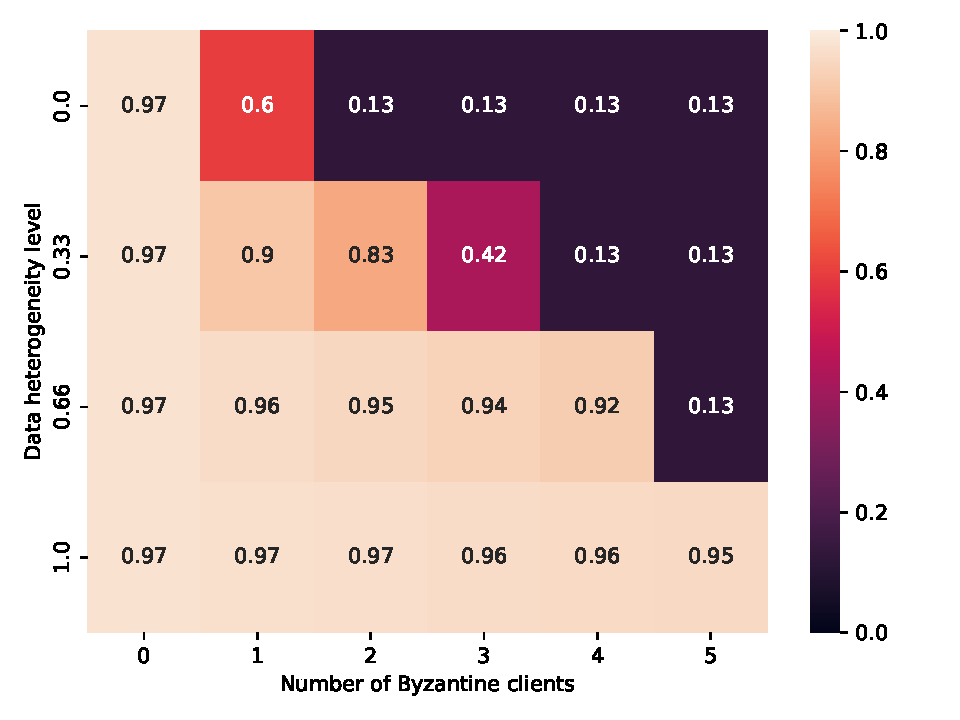
\includegraphics[width=\textwidth]{../plots/robust_new_atan_sweep/alpha_1.5/test_mnist_cnn_mnist_snn_gamma_similarity_niid_NNM_ARC_CenteredClipping_nb_honest_clients_10_tolerated_f_equal_real.pdf}
        \caption{$\alpha = 1.5$}
        \label{fig:cc_worst_case_alpha_1_5}
    \end{subfigure}
    \hfill
    \begin{subfigure}[b]{0.24\textwidth}
        \centering
        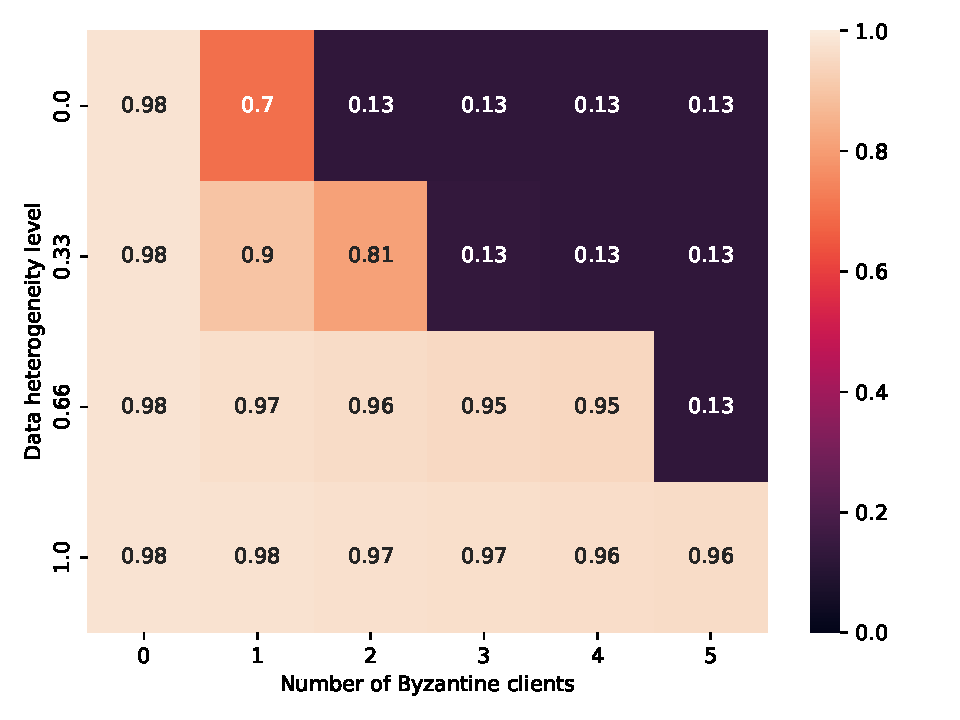
\includegraphics[width=\textwidth]{../plots/robust_new_atan_sweep/alpha_2.0/test_mnist_cnn_mnist_snn_gamma_similarity_niid_NNM_ARC_CenteredClipping_nb_honest_clients_10_tolerated_f_equal_real.pdf}
        \caption{$\alpha = 2.0$}
        \label{fig:cc_worst_case_alpha_2_0}
    \end{subfigure}
    \caption{Centered Clipping performance under the worst-case across all attacks across $\alpha$ values.}
    \label{fig:cc_worst_case_grid}
\end{figure}\clearpage
\subsubsection{CC under Optimal ALIE Attack}
\begin{figure}[htbp]
    \centering
    \begin{subfigure}[b]{0.24\textwidth}
        \centering
        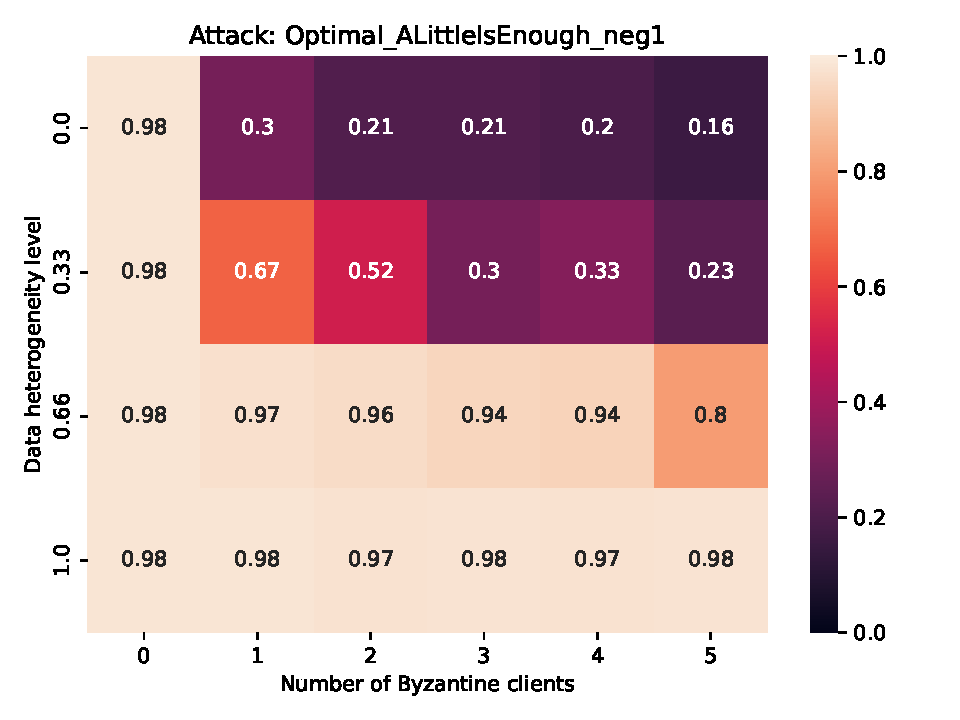
\includegraphics[width=\textwidth]{../plots/robust_comparison_sweep/test_Optimal_ALittleIsEnough_neg1_mnist_cnn_mnist_gamma_similarity_niid_NNM_ARC_CenteredClipping_nb_honest_clients_10_tolerated_f_equal_real.pdf}
        \caption{CNN Baseline}
        \label{fig:cc_alie_cnn}
    \end{subfigure}
    \hfill
    \begin{subfigure}[b]{0.24\textwidth}
        \centering
        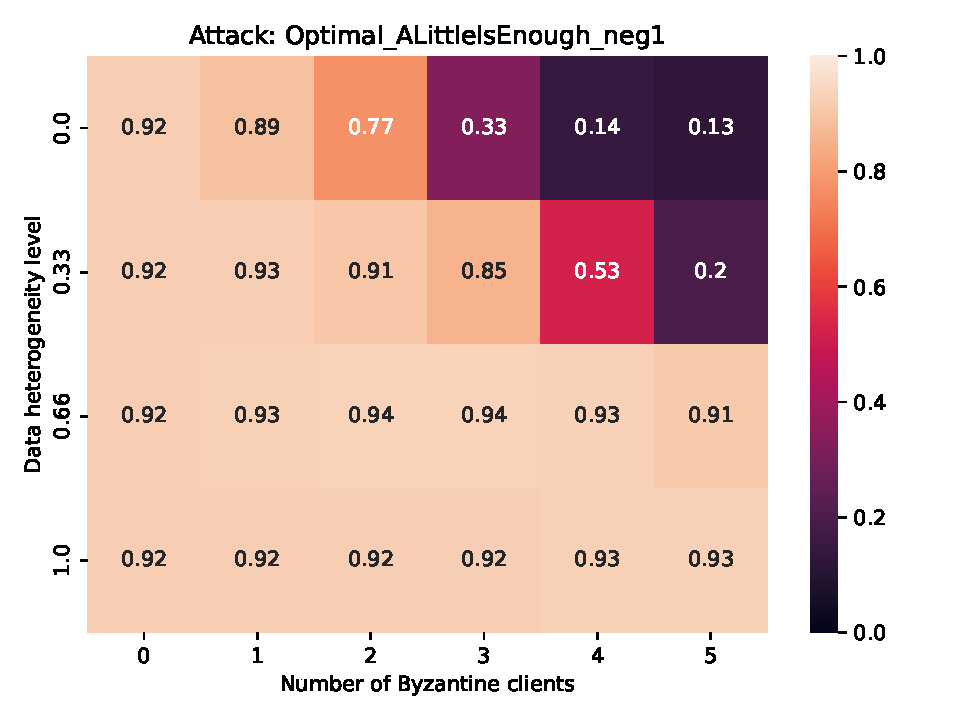
\includegraphics[width=\textwidth]{../plots/robust_new_atan_sweep/alpha_0.5/test_Optimal_ALittleIsEnough_neg1_mnist_cnn_mnist_snn_gamma_similarity_niid_NNM_ARC_CenteredClipping_nb_honest_clients_10_tolerated_f_equal_real.pdf}
        \caption{$\alpha = 0.5$}
        \label{fig:cc_alie_alpha_0_5}
    \end{subfigure}
    \hfill
    \begin{subfigure}[b]{0.24\textwidth}
        \centering
        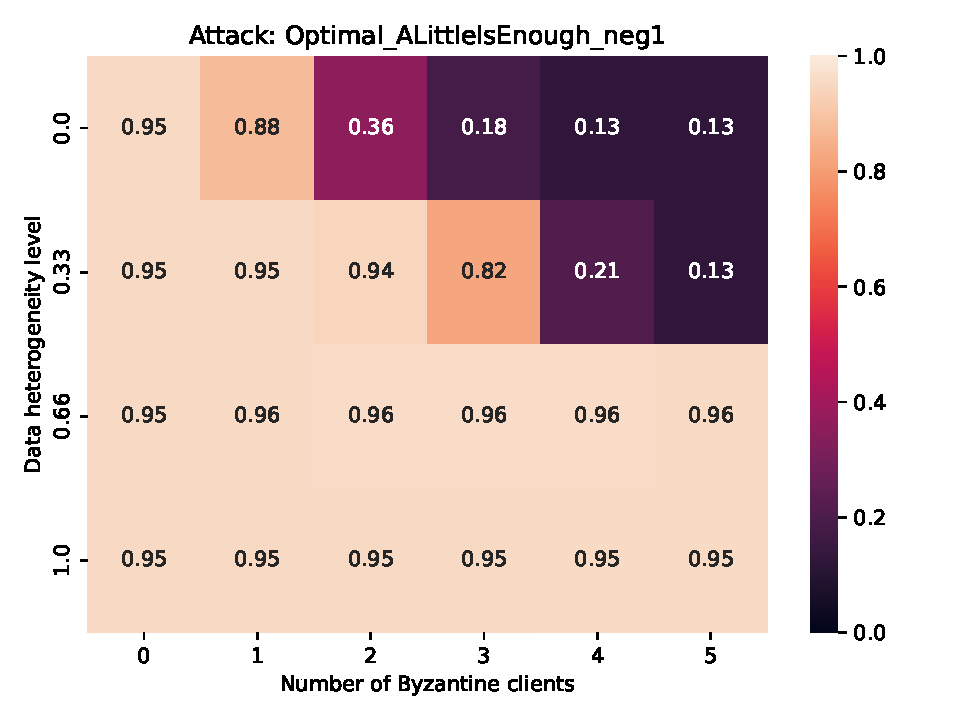
\includegraphics[width=\textwidth]{../plots/robust_new_atan_sweep/alpha_0.75/test_Optimal_ALittleIsEnough_neg1_mnist_cnn_mnist_snn_gamma_similarity_niid_NNM_ARC_CenteredClipping_nb_honest_clients_10_tolerated_f_equal_real.pdf}
        \caption{$\alpha = 0.75$}
        \label{fig:cc_alie_alpha_0_75}
    \end{subfigure}
    \hfill
    \begin{subfigure}[b]{0.24\textwidth}
        \centering
        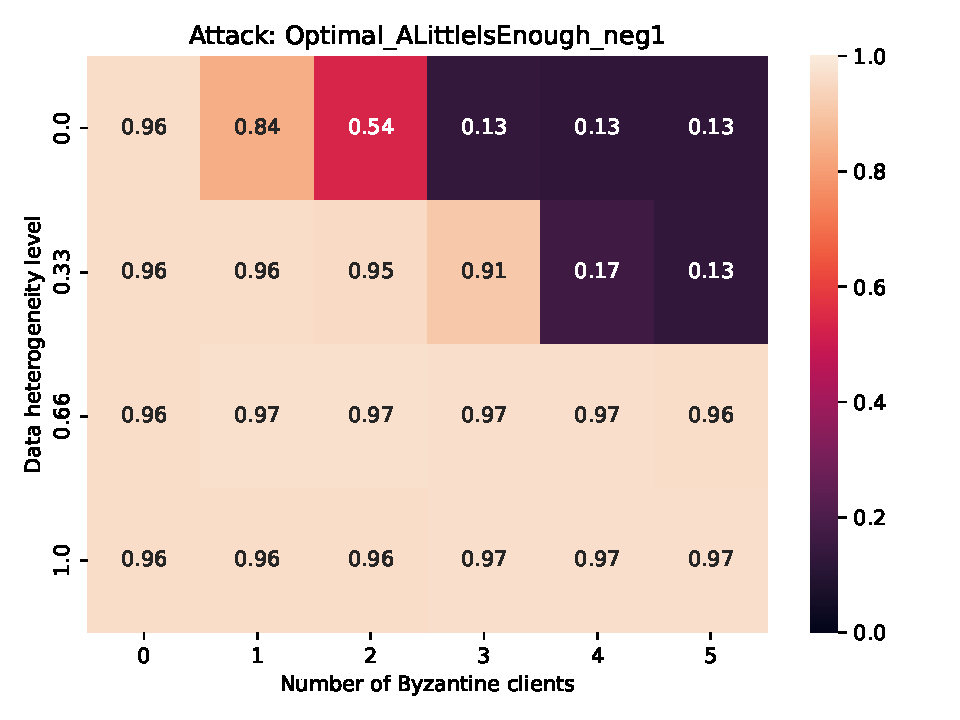
\includegraphics[width=\textwidth]{../plots/robust_new_atan_sweep/alpha_1.0/test_Optimal_ALittleIsEnough_neg1_mnist_cnn_mnist_snn_gamma_similarity_niid_NNM_ARC_CenteredClipping_nb_honest_clients_10_tolerated_f_equal_real.pdf}
        \caption{$\alpha = 1.0$}
        \label{fig:cc_alie_alpha_1_0}
    \end{subfigure}
    \vspace{0.2cm}
    \begin{subfigure}[b]{0.24\textwidth}
        \centering
        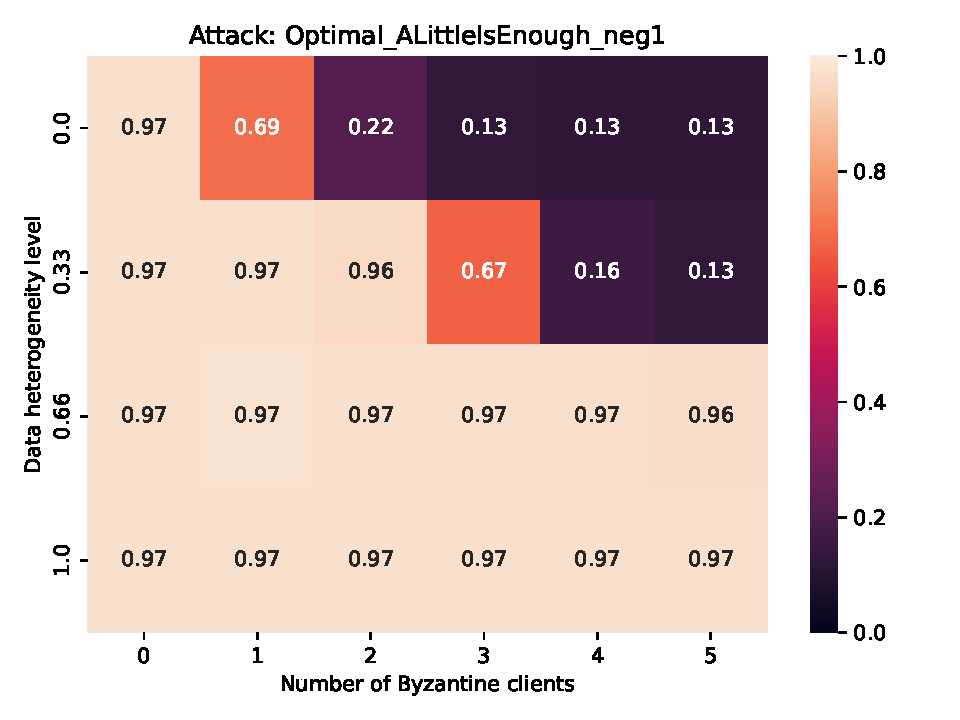
\includegraphics[width=\textwidth]{../plots/robust_new_atan_sweep/alpha_1.2/test_Optimal_ALittleIsEnough_neg1_mnist_cnn_mnist_snn_gamma_similarity_niid_NNM_ARC_CenteredClipping_nb_honest_clients_10_tolerated_f_equal_real.pdf}
        \caption{$\alpha = 1.2$}
        \label{fig:cc_alie_alpha_1_2}
    \end{subfigure}
    \hfill
    \begin{subfigure}[b]{0.24\textwidth}
        \centering
        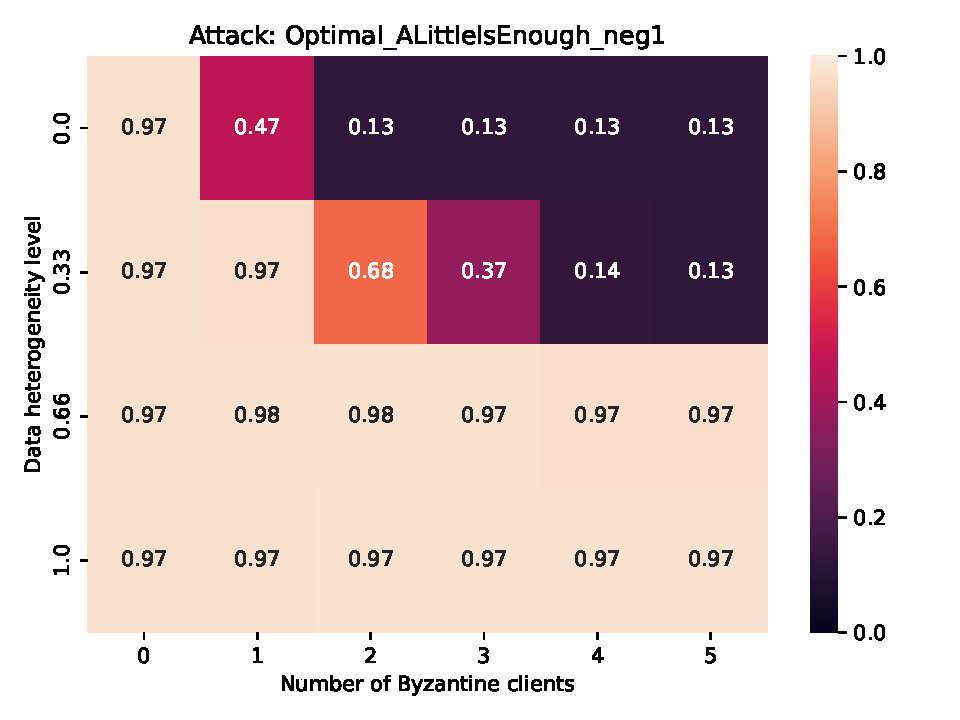
\includegraphics[width=\textwidth]{../plots/robust_new_atan_sweep/alpha_1.4/test_Optimal_ALittleIsEnough_neg1_mnist_cnn_mnist_snn_gamma_similarity_niid_NNM_ARC_CenteredClipping_nb_honest_clients_10_tolerated_f_equal_real.pdf}
        \caption{$\alpha = 1.4$}
        \label{fig:cc_alie_alpha_1_4}
    \end{subfigure}
    \hfill
    \begin{subfigure}[b]{0.24\textwidth}
        \centering
        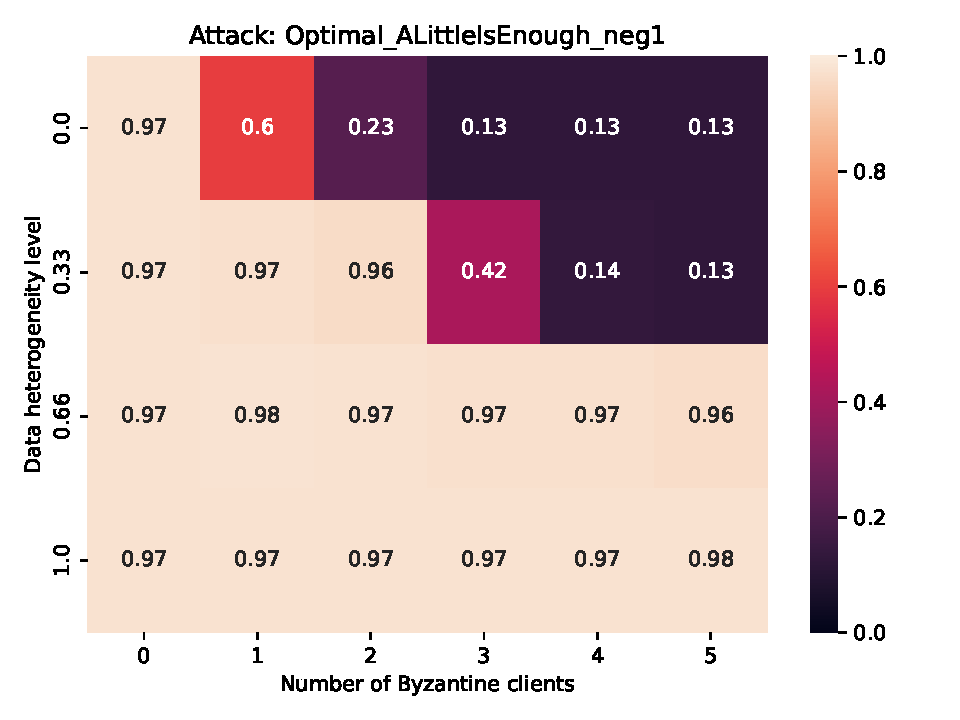
\includegraphics[width=\textwidth]{../plots/robust_new_atan_sweep/alpha_1.5/test_Optimal_ALittleIsEnough_neg1_mnist_cnn_mnist_snn_gamma_similarity_niid_NNM_ARC_CenteredClipping_nb_honest_clients_10_tolerated_f_equal_real.pdf}
        \caption{$\alpha = 1.5$}
        \label{fig:cc_alie_alpha_1_5}
    \end{subfigure}
    \hfill
    \begin{subfigure}[b]{0.24\textwidth}
        \centering
        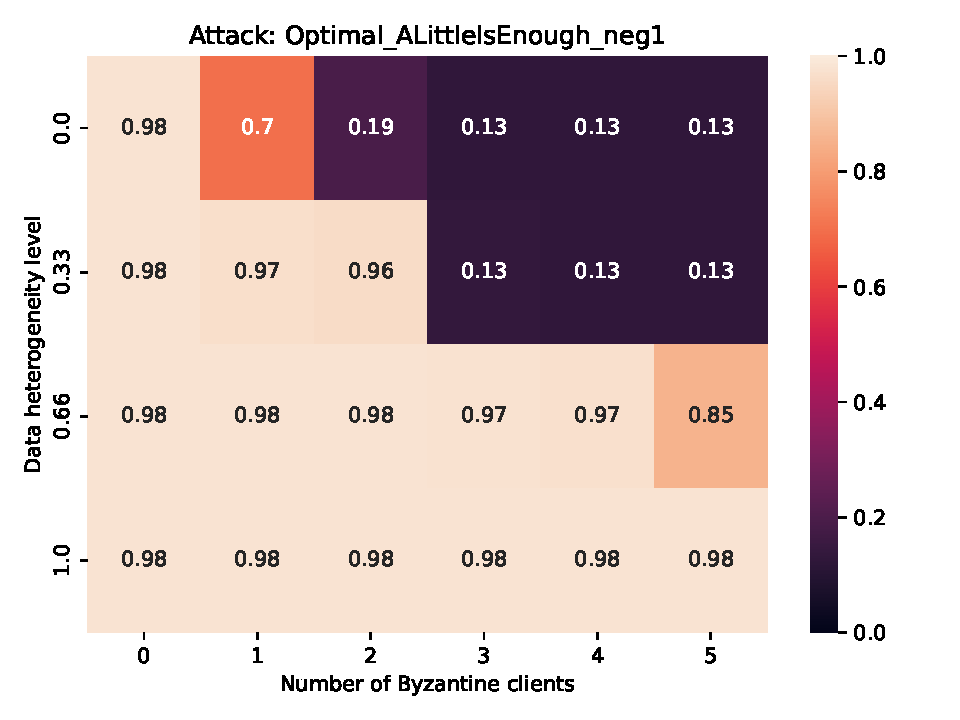
\includegraphics[width=\textwidth]{../plots/robust_new_atan_sweep/alpha_2.0/test_Optimal_ALittleIsEnough_neg1_mnist_cnn_mnist_snn_gamma_similarity_niid_NNM_ARC_CenteredClipping_nb_honest_clients_10_tolerated_f_equal_real.pdf}
        \caption{$\alpha = 2.0$}
        \label{fig:cc_alie_alpha_2_0}
    \end{subfigure}
    \caption{Centered Clipping performance under Optimal ALIE across $\alpha$ values.}
    \label{fig:cc_alie_grid}
\end{figure}\clearpage
\subsubsection{CC under Sign Flipping Attack}
\begin{figure}[htbp]
    \centering
    \begin{subfigure}[b]{0.24\textwidth}
        \centering
        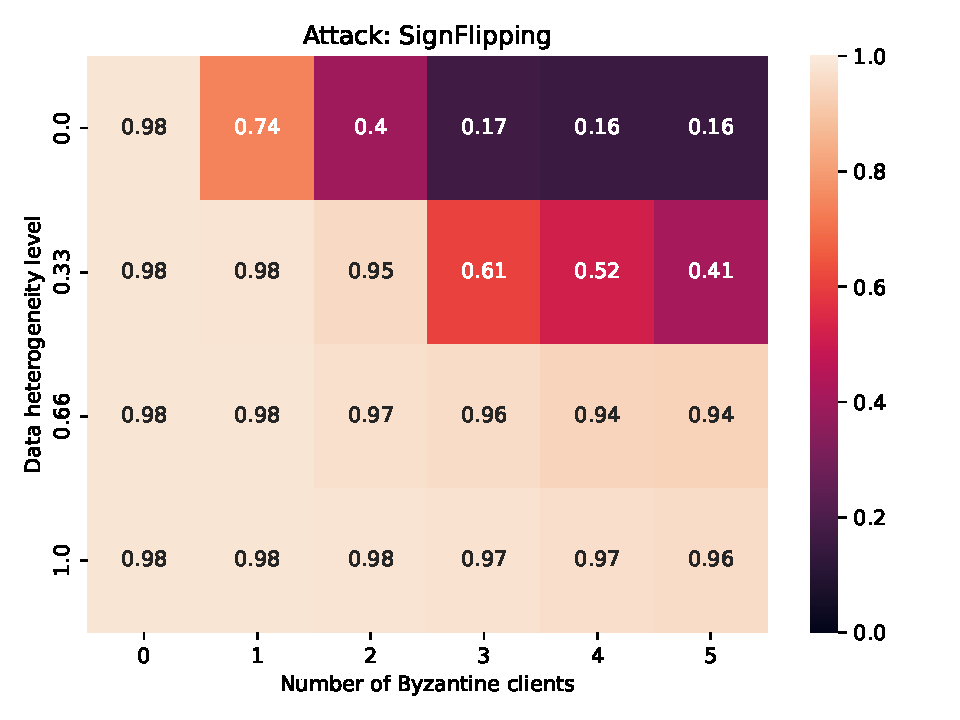
\includegraphics[width=\textwidth]{../plots/robust_comparison_sweep/test_SignFlipping_mnist_cnn_mnist_gamma_similarity_niid_NNM_ARC_CenteredClipping_nb_honest_clients_10_tolerated_f_equal_real.pdf}
        \caption{CNN Baseline}
        \label{fig:cc_sf_cnn}
    \end{subfigure}
    \hfill
    \begin{subfigure}[b]{0.24\textwidth}
        \centering
        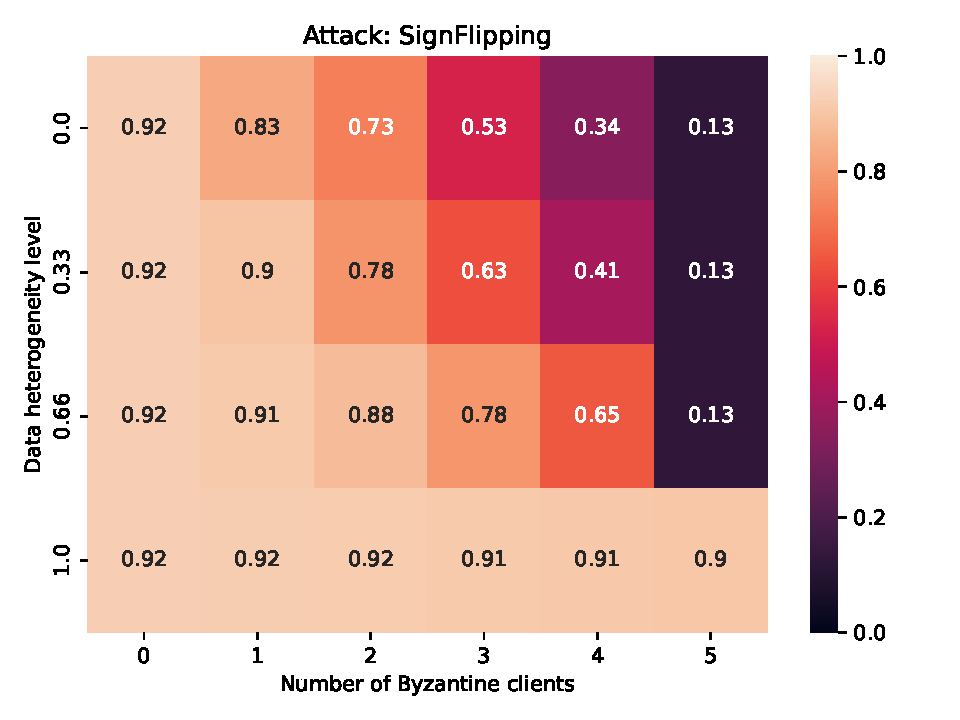
\includegraphics[width=\textwidth]{../plots/robust_new_atan_sweep/alpha_0.5/test_SignFlipping_mnist_cnn_mnist_snn_gamma_similarity_niid_NNM_ARC_CenteredClipping_nb_honest_clients_10_tolerated_f_equal_real.pdf}
        \caption{$\alpha = 0.5$}
        \label{fig:cc_sf_alpha_0_5}
    \end{subfigure}
    \hfill
    \begin{subfigure}[b]{0.24\textwidth}
        \centering
        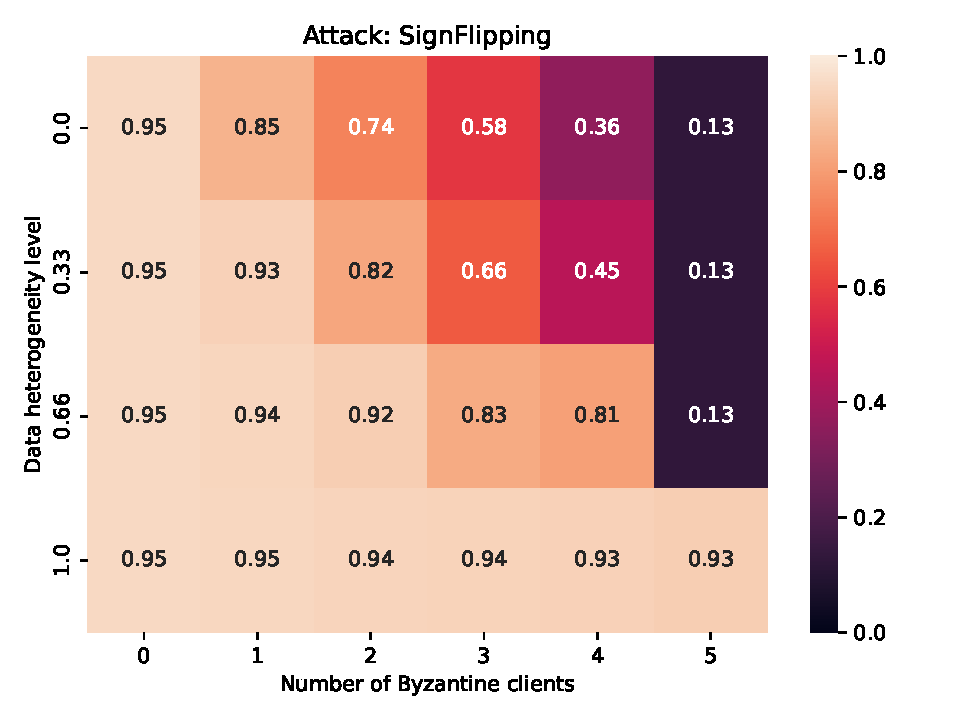
\includegraphics[width=\textwidth]{../plots/robust_new_atan_sweep/alpha_0.75/test_SignFlipping_mnist_cnn_mnist_snn_gamma_similarity_niid_NNM_ARC_CenteredClipping_nb_honest_clients_10_tolerated_f_equal_real.pdf}
        \caption{$\alpha = 0.75$}
        \label{fig:cc_sf_alpha_0_75}
    \end{subfigure}
    \hfill
    \begin{subfigure}[b]{0.24\textwidth}
        \centering
        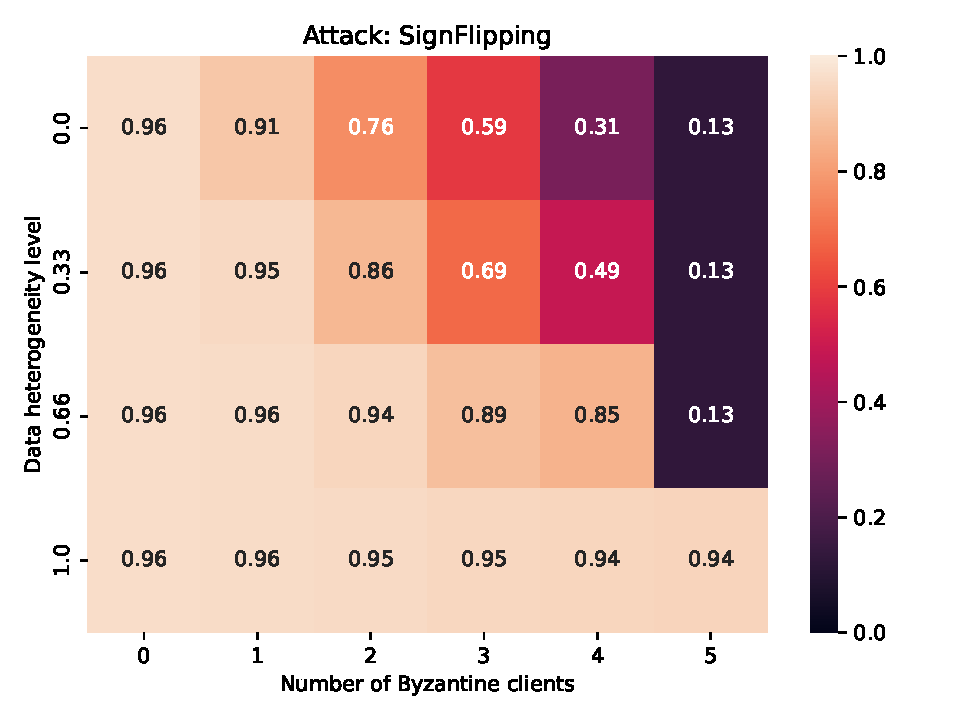
\includegraphics[width=\textwidth]{../plots/robust_new_atan_sweep/alpha_1.0/test_SignFlipping_mnist_cnn_mnist_snn_gamma_similarity_niid_NNM_ARC_CenteredClipping_nb_honest_clients_10_tolerated_f_equal_real.pdf}
        \caption{$\alpha = 1.0$}
        \label{fig:cc_sf_alpha_1_0}
    \end{subfigure}
    \vspace{0.2cm}
    \begin{subfigure}[b]{0.24\textwidth}
        \centering
        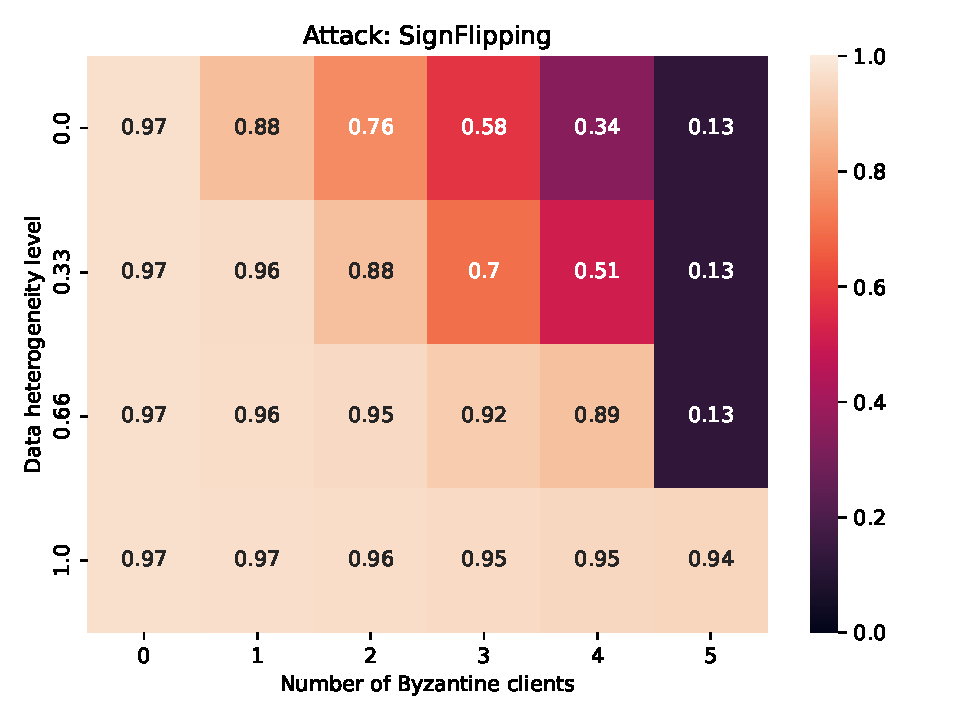
\includegraphics[width=\textwidth]{../plots/robust_new_atan_sweep/alpha_1.2/test_SignFlipping_mnist_cnn_mnist_snn_gamma_similarity_niid_NNM_ARC_CenteredClipping_nb_honest_clients_10_tolerated_f_equal_real.pdf}
        \caption{$\alpha = 1.2$}
        \label{fig:cc_sf_alpha_1_2}
    \end{subfigure}
    \hfill
    \begin{subfigure}[b]{0.24\textwidth}
        \centering
        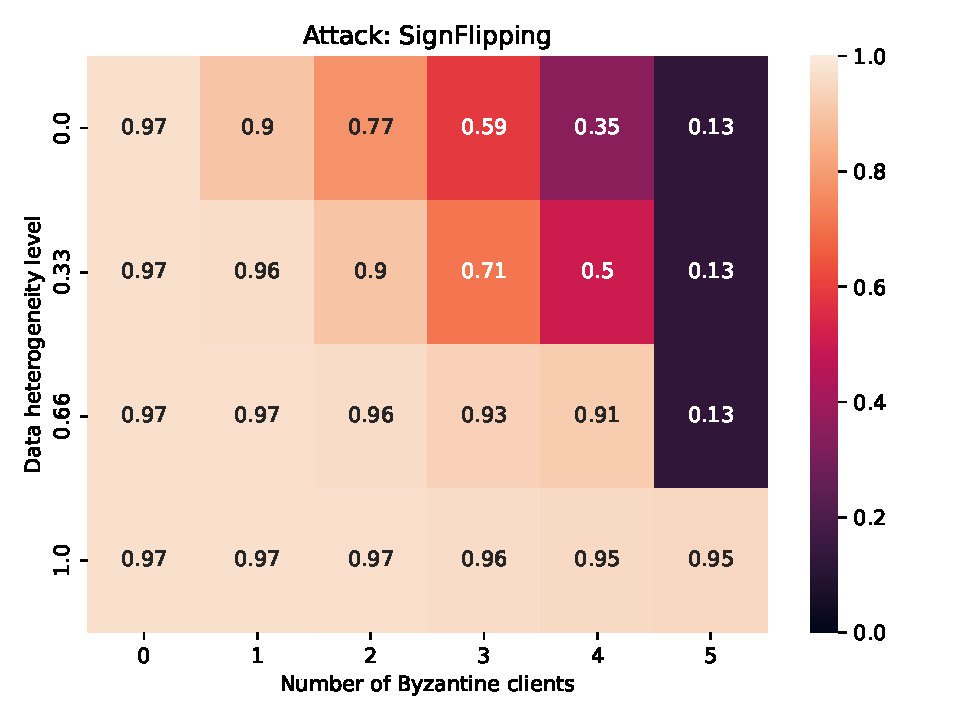
\includegraphics[width=\textwidth]{../plots/robust_new_atan_sweep/alpha_1.4/test_SignFlipping_mnist_cnn_mnist_snn_gamma_similarity_niid_NNM_ARC_CenteredClipping_nb_honest_clients_10_tolerated_f_equal_real.pdf}
        \caption{$\alpha = 1.4$}
        \label{fig:cc_sf_alpha_1_4}
    \end{subfigure}
    \hfill
    \begin{subfigure}[b]{0.24\textwidth}
        \centering
        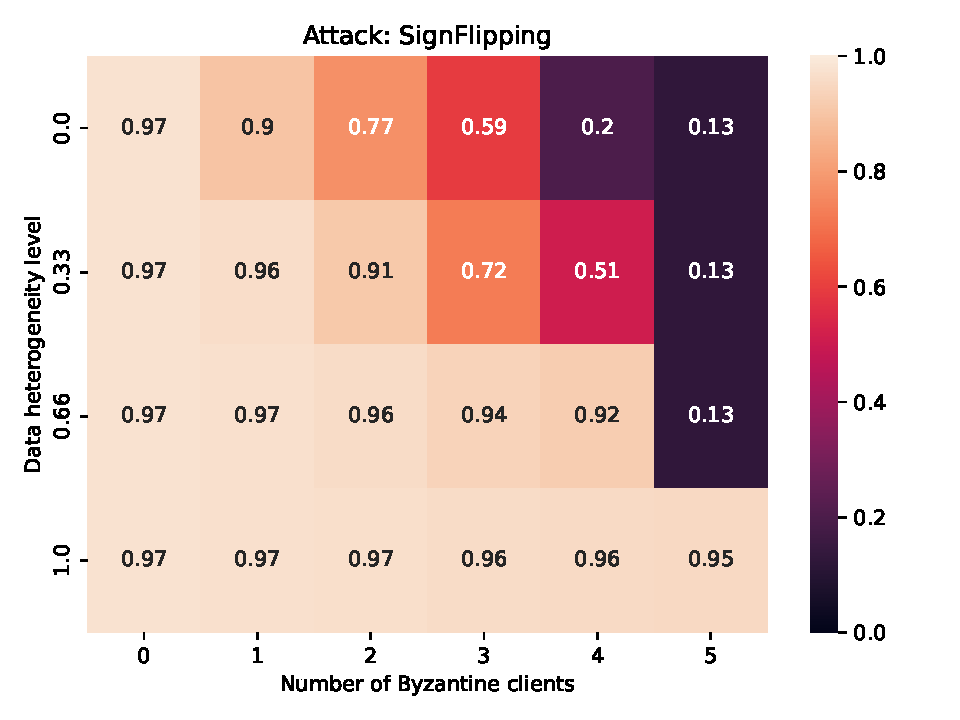
\includegraphics[width=\textwidth]{../plots/robust_new_atan_sweep/alpha_1.5/test_SignFlipping_mnist_cnn_mnist_snn_gamma_similarity_niid_NNM_ARC_CenteredClipping_nb_honest_clients_10_tolerated_f_equal_real.pdf}
        \caption{$\alpha = 1.5$}
        \label{fig:cc_sf_alpha_1_5}
    \end{subfigure}
    \hfill
    \begin{subfigure}[b]{0.24\textwidth}
        \centering
        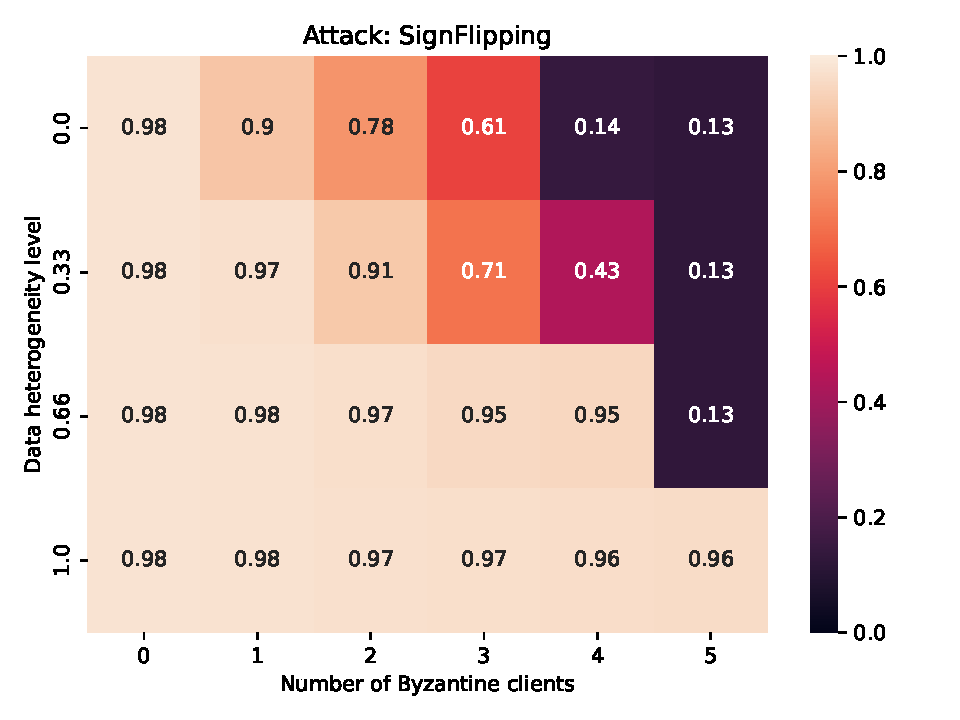
\includegraphics[width=\textwidth]{../plots/robust_new_atan_sweep/alpha_2.0/test_SignFlipping_mnist_cnn_mnist_snn_gamma_similarity_niid_NNM_ARC_CenteredClipping_nb_honest_clients_10_tolerated_f_equal_real.pdf}
        \caption{$\alpha = 2.0$}
        \label{fig:cc_sf_alpha_2_0}
    \end{subfigure}
    \caption{Centered Clipping performance under Sign Flipping across $\alpha$ values.}
    \label{fig:cc_sf_grid}
\end{figure}\clearpage
\subsubsection{CC under Optimal Inner Product Manipulation Attack}
\begin{figure}[htbp]
    \centering
    \begin{subfigure}[b]{0.24\textwidth}
        \centering
        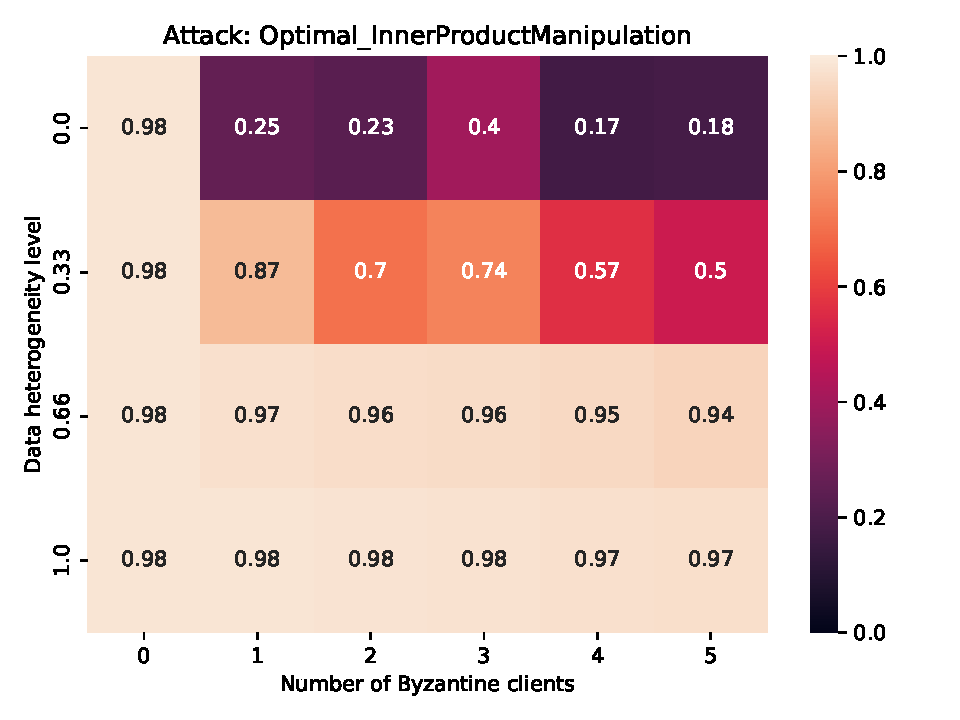
\includegraphics[width=\textwidth]{../plots/robust_comparison_sweep/test_Optimal_InnerProductManipulation_mnist_cnn_mnist_gamma_similarity_niid_NNM_ARC_CenteredClipping_nb_honest_clients_10_tolerated_f_equal_real.pdf}
        \caption{CNN Baseline}
        \label{fig:cc_ipm_cnn}
    \end{subfigure}
    \hfill
    \begin{subfigure}[b]{0.24\textwidth}
        \centering
        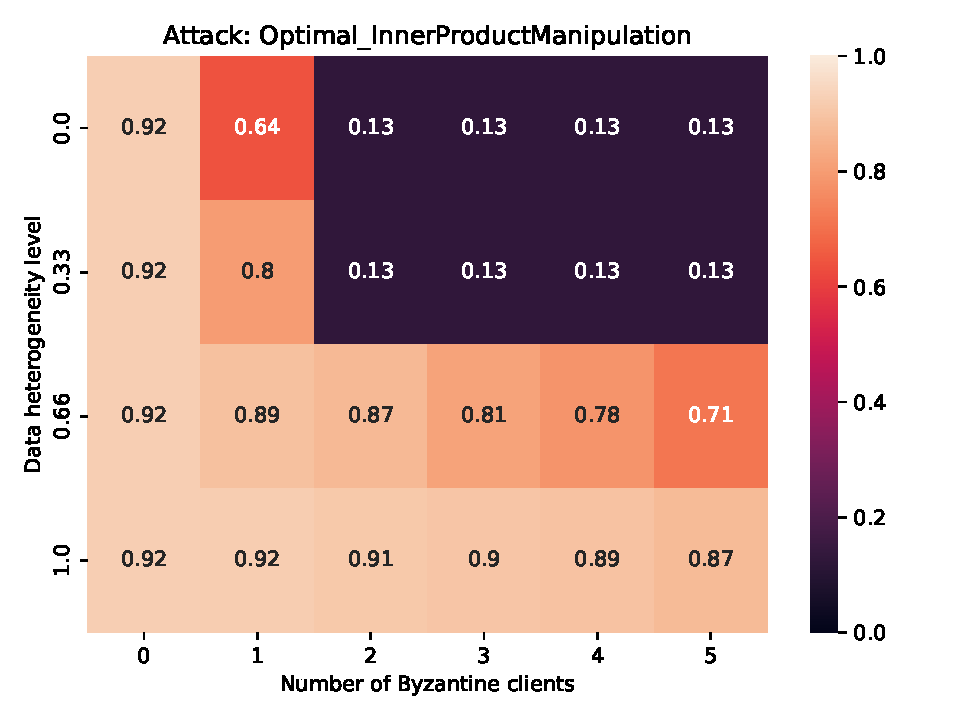
\includegraphics[width=\textwidth]{../plots/robust_new_atan_sweep/alpha_0.5/test_Optimal_InnerProductManipulation_mnist_cnn_mnist_snn_gamma_similarity_niid_NNM_ARC_CenteredClipping_nb_honest_clients_10_tolerated_f_equal_real.pdf}
        \caption{$\alpha = 0.5$}
        \label{fig:cc_ipm_alpha_0_5}
    \end{subfigure}
    \hfill
    \begin{subfigure}[b]{0.24\textwidth}
        \centering
        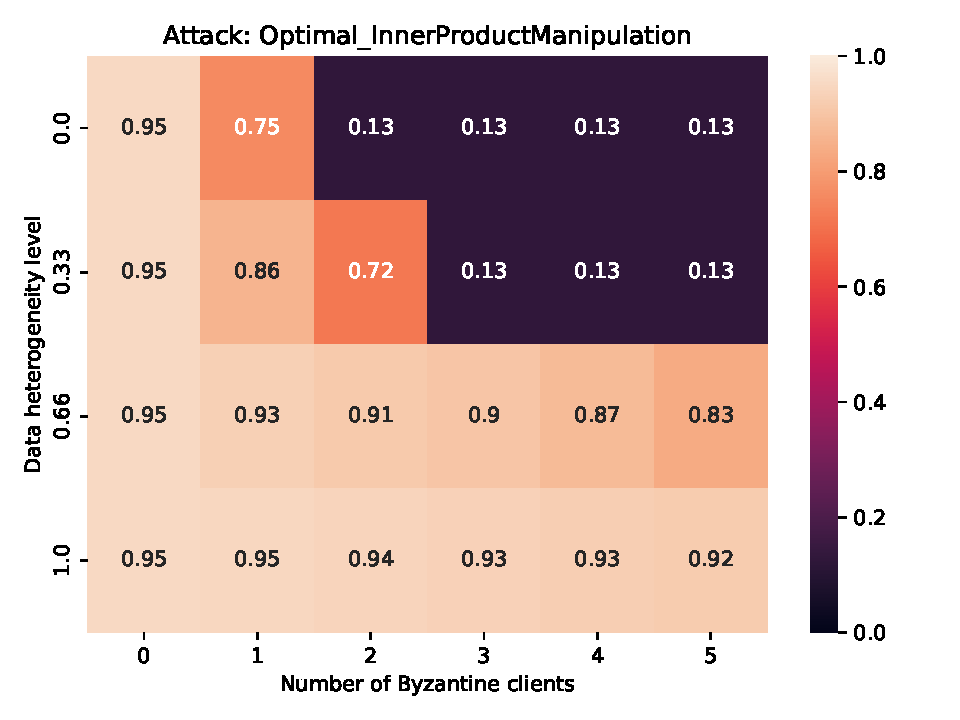
\includegraphics[width=\textwidth]{../plots/robust_new_atan_sweep/alpha_0.75/test_Optimal_InnerProductManipulation_mnist_cnn_mnist_snn_gamma_similarity_niid_NNM_ARC_CenteredClipping_nb_honest_clients_10_tolerated_f_equal_real.pdf}
        \caption{$\alpha = 0.75$}
        \label{fig:cc_ipm_alpha_0_75}
    \end{subfigure}
    \hfill
    \begin{subfigure}[b]{0.24\textwidth}
        \centering
        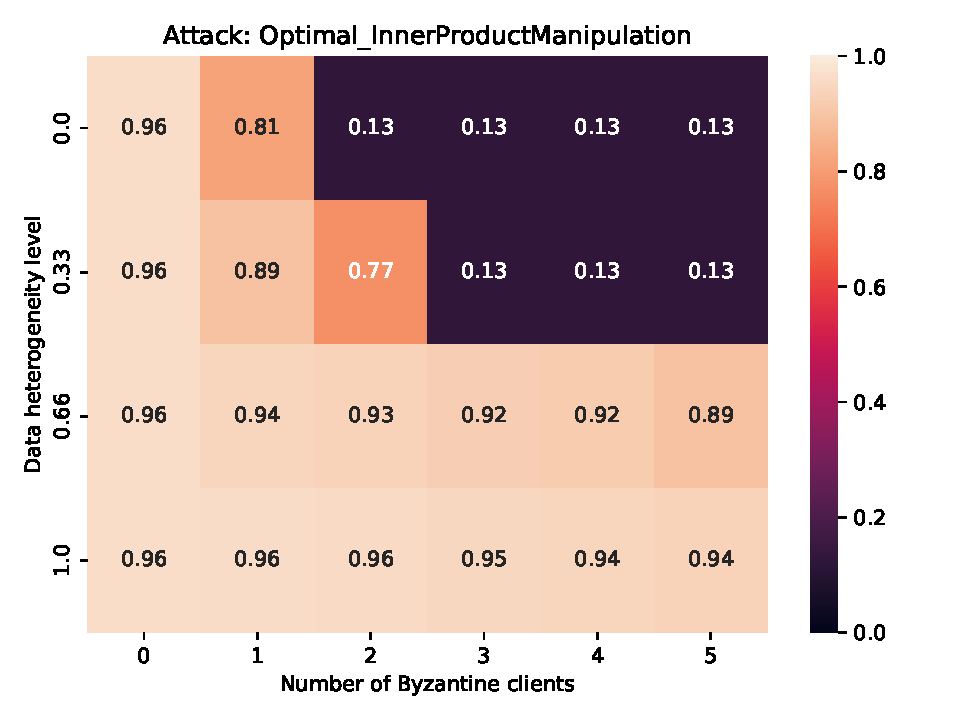
\includegraphics[width=\textwidth]{../plots/robust_new_atan_sweep/alpha_1.0/test_Optimal_InnerProductManipulation_mnist_cnn_mnist_snn_gamma_similarity_niid_NNM_ARC_CenteredClipping_nb_honest_clients_10_tolerated_f_equal_real.pdf}
        \caption{$\alpha = 1.0$}
        \label{fig:cc_ipm_alpha_1_0}
    \end{subfigure}
    \vspace{0.2cm}
    \begin{subfigure}[b]{0.24\textwidth}
        \centering
        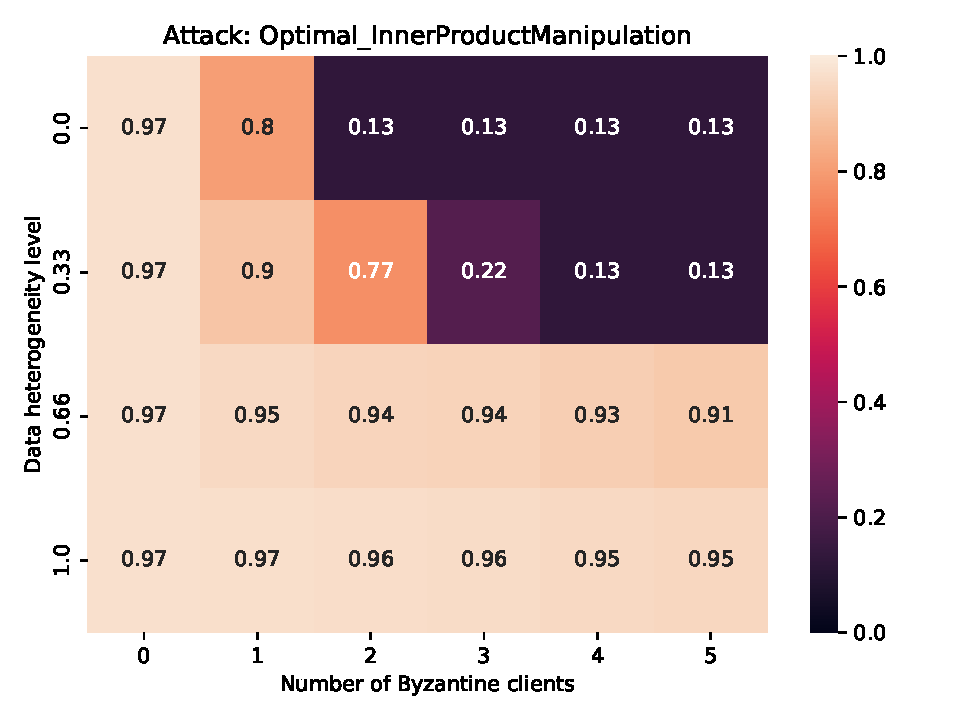
\includegraphics[width=\textwidth]{../plots/robust_new_atan_sweep/alpha_1.2/test_Optimal_InnerProductManipulation_mnist_cnn_mnist_snn_gamma_similarity_niid_NNM_ARC_CenteredClipping_nb_honest_clients_10_tolerated_f_equal_real.pdf}
        \caption{$\alpha = 1.2$}
        \label{fig:cc_ipm_alpha_1_2}
    \end{subfigure}
    \hfill
    \begin{subfigure}[b]{0.24\textwidth}
        \centering
        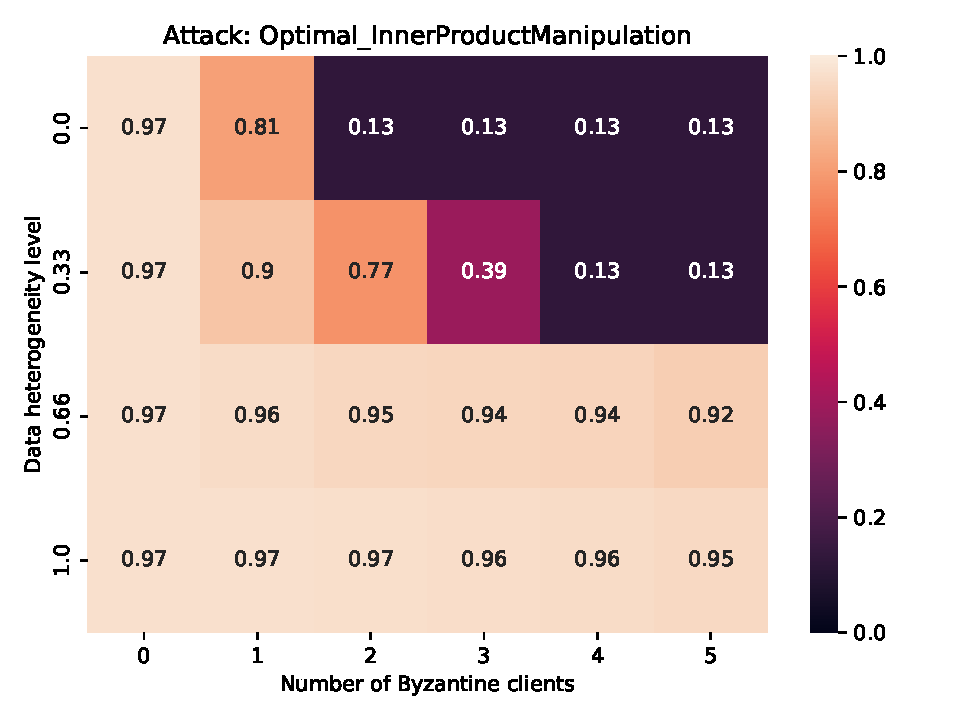
\includegraphics[width=\textwidth]{../plots/robust_new_atan_sweep/alpha_1.4/test_Optimal_InnerProductManipulation_mnist_cnn_mnist_snn_gamma_similarity_niid_NNM_ARC_CenteredClipping_nb_honest_clients_10_tolerated_f_equal_real.pdf}
        \caption{$\alpha = 1.4$}
        \label{fig:cc_ipm_alpha_1_4}
    \end{subfigure}
    \hfill
    \begin{subfigure}[b]{0.24\textwidth}
        \centering
        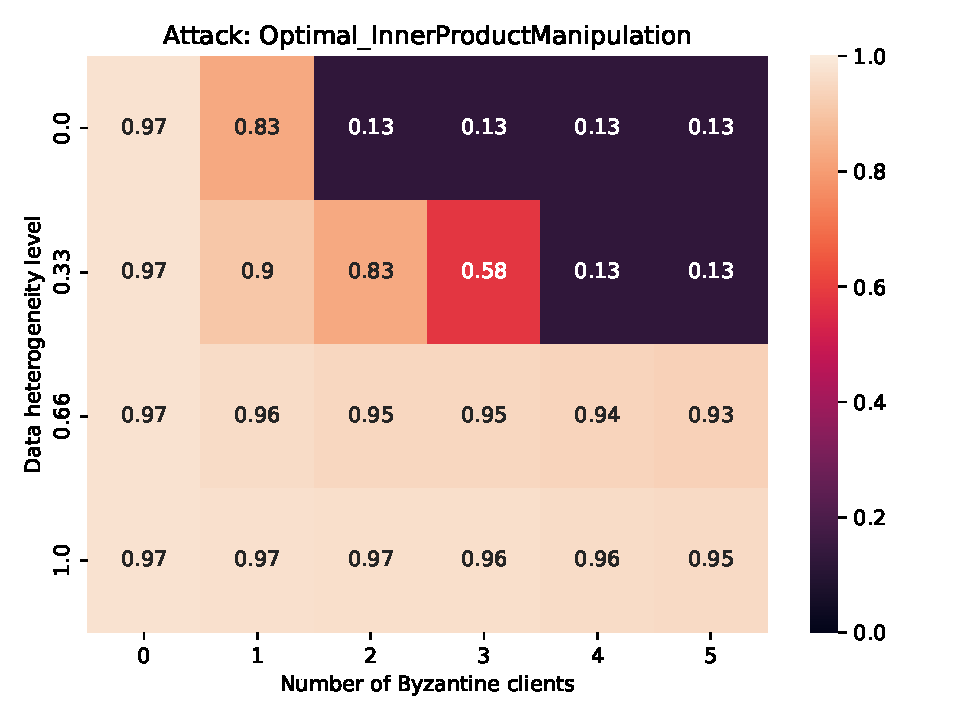
\includegraphics[width=\textwidth]{../plots/robust_new_atan_sweep/alpha_1.5/test_Optimal_InnerProductManipulation_mnist_cnn_mnist_snn_gamma_similarity_niid_NNM_ARC_CenteredClipping_nb_honest_clients_10_tolerated_f_equal_real.pdf}
        \caption{$\alpha = 1.5$}
        \label{fig:cc_ipm_alpha_1_5}
    \end{subfigure}
    \hfill
    \begin{subfigure}[b]{0.24\textwidth}
        \centering
        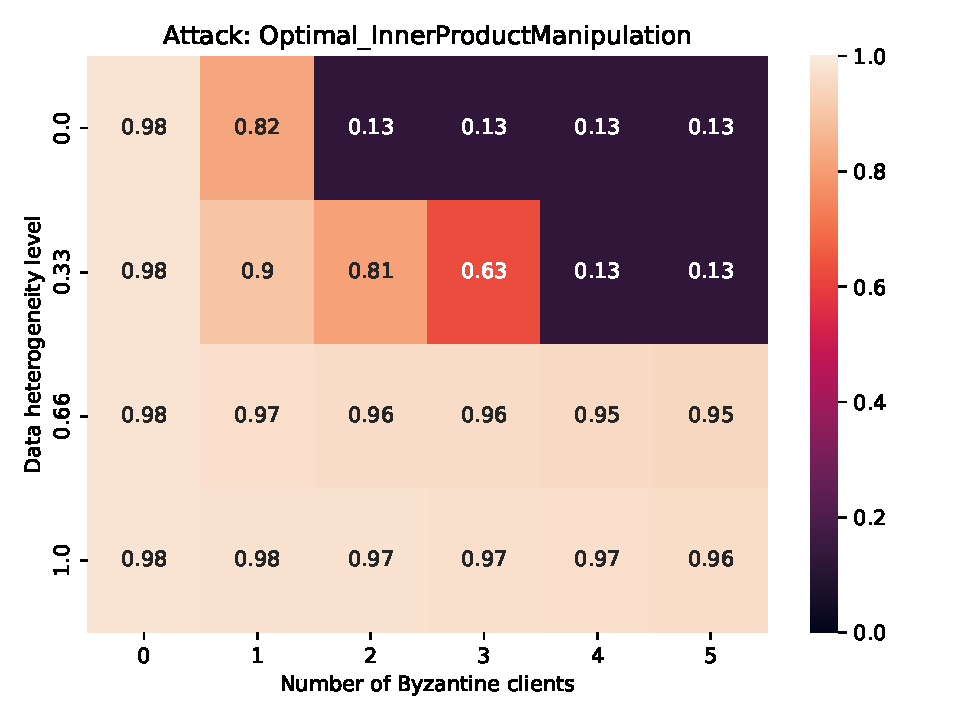
\includegraphics[width=\textwidth]{../plots/robust_new_atan_sweep/alpha_2.0/test_Optimal_InnerProductManipulation_mnist_cnn_mnist_snn_gamma_similarity_niid_NNM_ARC_CenteredClipping_nb_honest_clients_10_tolerated_f_equal_real.pdf}
        \caption{$\alpha = 2.0$}
        \label{fig:cc_ipm_alpha_2_0}
    \end{subfigure}
    \caption{Centered Clipping performance under Optimal Inner Product Manipulation across $\alpha$ values.}
    \label{fig:cc_ipm_grid}
\end{figure}
\clearpage
\subsection{Geometric Median (GM)}
\subsubsection{GM under Worst-Case across all Attacks}
\begin{figure}[htbp]
    \centering
    \begin{subfigure}[b]{0.24\textwidth}
        \centering
        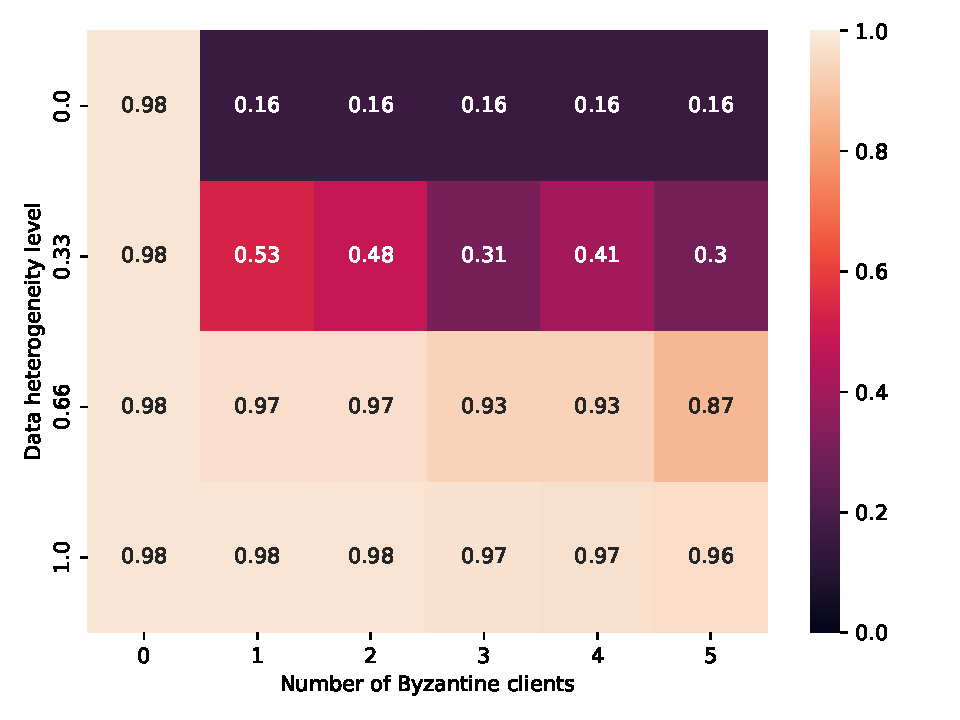
\includegraphics[width=\textwidth]{../plots/robust_comparison_sweep/test_mnist_cnn_mnist_gamma_similarity_niid_NNM_ARC_GeometricMedian_nb_honest_clients_10_tolerated_f_equal_real.pdf}
        \caption{CNN Baseline}
        \label{fig:gm_worst_case_cnn}
    \end{subfigure}
    \hfill
    \begin{subfigure}[b]{0.24\textwidth}
        \centering
        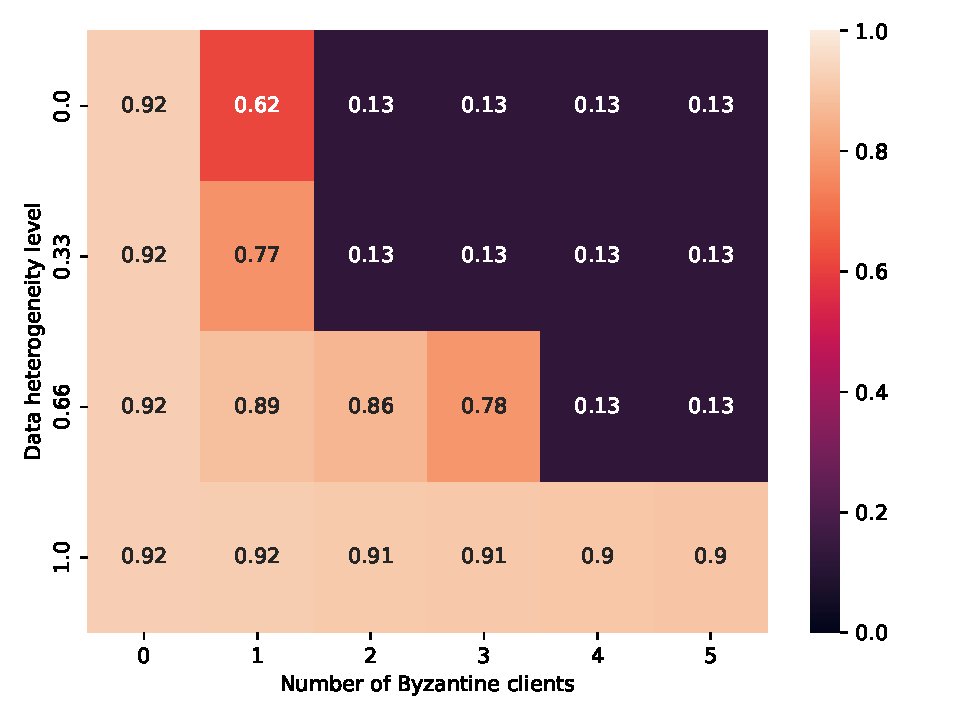
\includegraphics[width=\textwidth]{../plots/robust_new_atan_sweep/alpha_0.5/test_mnist_cnn_mnist_snn_gamma_similarity_niid_NNM_ARC_GeometricMedian_nb_honest_clients_10_tolerated_f_equal_real.pdf}
        \caption{$\alpha = 0.5$}
        \label{fig:gm_worst_case_alpha_0_5}
    \end{subfigure}
    \hfill
    \begin{subfigure}[b]{0.24\textwidth}
        \centering
        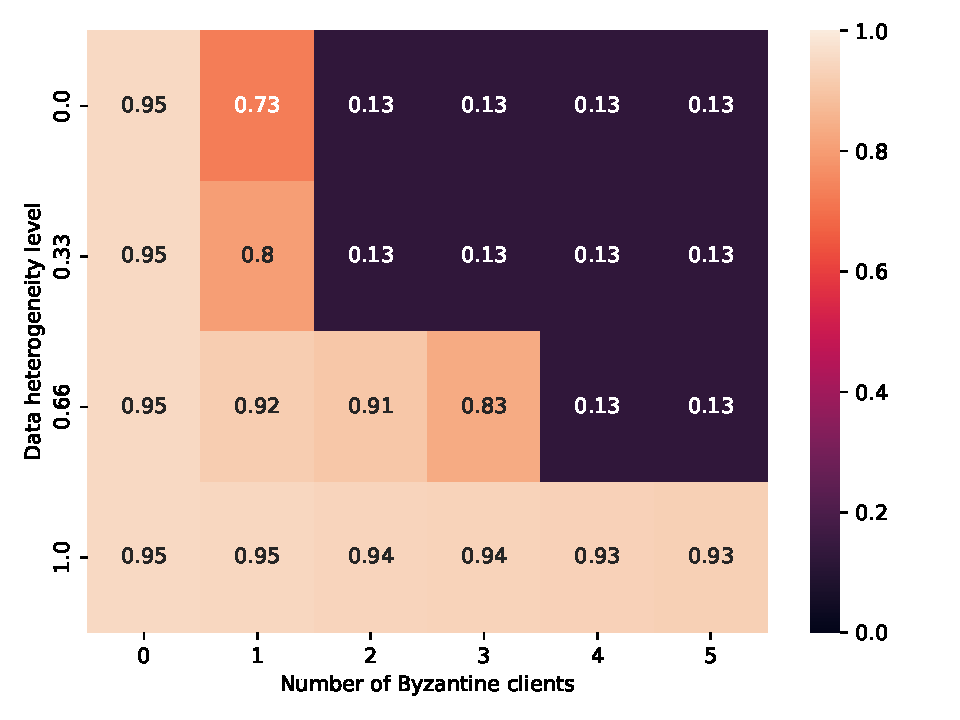
\includegraphics[width=\textwidth]{../plots/robust_new_atan_sweep/alpha_0.75/test_mnist_cnn_mnist_snn_gamma_similarity_niid_NNM_ARC_GeometricMedian_nb_honest_clients_10_tolerated_f_equal_real.pdf}
        \caption{$\alpha = 0.75$}
        \label{fig:gm_worst_case_alpha_0_75}
    \end{subfigure}
    \hfill
    \begin{subfigure}[b]{0.24\textwidth}
        \centering
        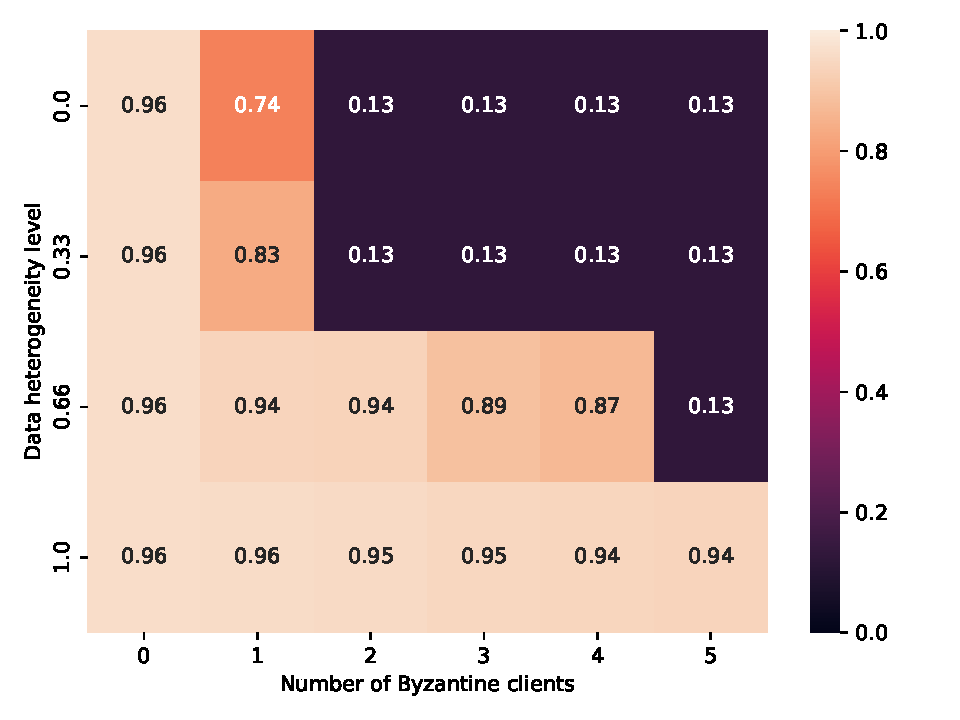
\includegraphics[width=\textwidth]{../plots/robust_new_atan_sweep/alpha_1.0/test_mnist_cnn_mnist_snn_gamma_similarity_niid_NNM_ARC_GeometricMedian_nb_honest_clients_10_tolerated_f_equal_real.pdf}
        \caption{$\alpha = 1.0$}
        \label{fig:gm_worst_case_alpha_1_0}
    \end{subfigure}
    \vspace{0.2cm}
    \begin{subfigure}[b]{0.24\textwidth}
        \centering
        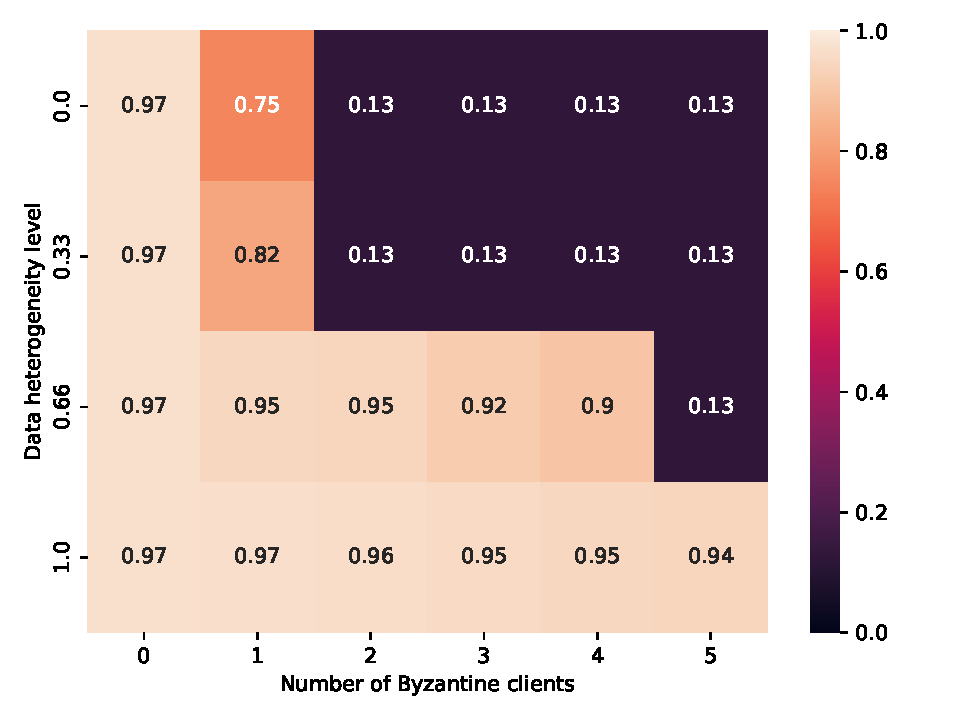
\includegraphics[width=\textwidth]{../plots/robust_new_atan_sweep/alpha_1.2/test_mnist_cnn_mnist_snn_gamma_similarity_niid_NNM_ARC_GeometricMedian_nb_honest_clients_10_tolerated_f_equal_real.pdf}
        \caption{$\alpha = 1.2$}
        \label{fig:gm_worst_case_alpha_1_2}
    \end{subfigure}
    \hfill
    \begin{subfigure}[b]{0.24\textwidth}
        \centering
        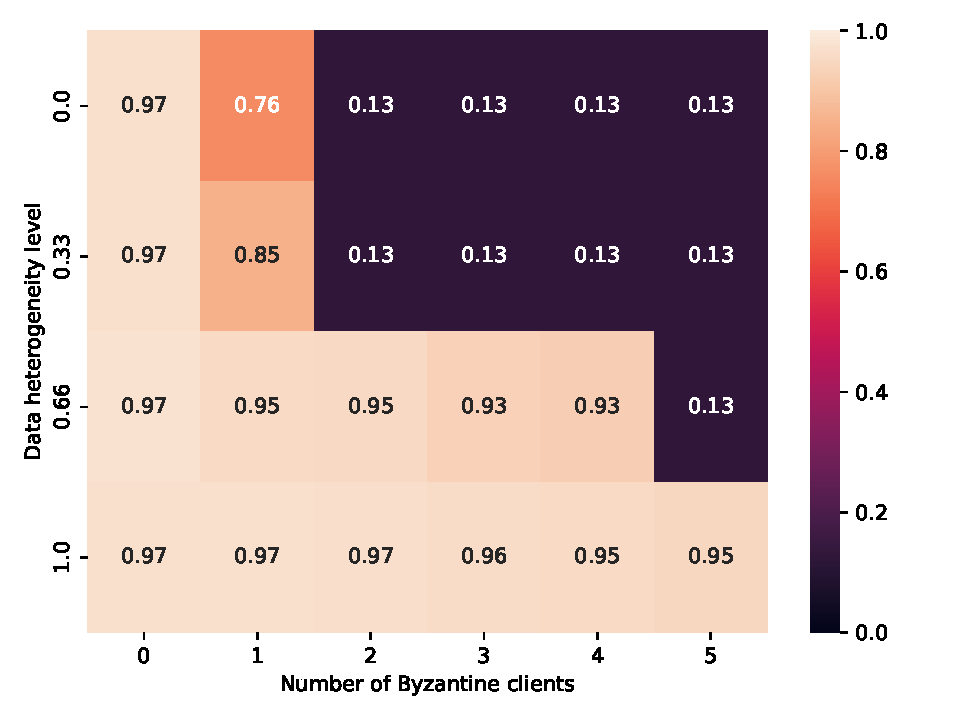
\includegraphics[width=\textwidth]{../plots/robust_new_atan_sweep/alpha_1.4/test_mnist_cnn_mnist_snn_gamma_similarity_niid_NNM_ARC_GeometricMedian_nb_honest_clients_10_tolerated_f_equal_real.pdf}
        \caption{$\alpha = 1.4$}
        \label{fig:gm_worst_case_alpha_1_4}
    \end{subfigure}
    \hfill
    \begin{subfigure}[b]{0.24\textwidth}
        \centering
        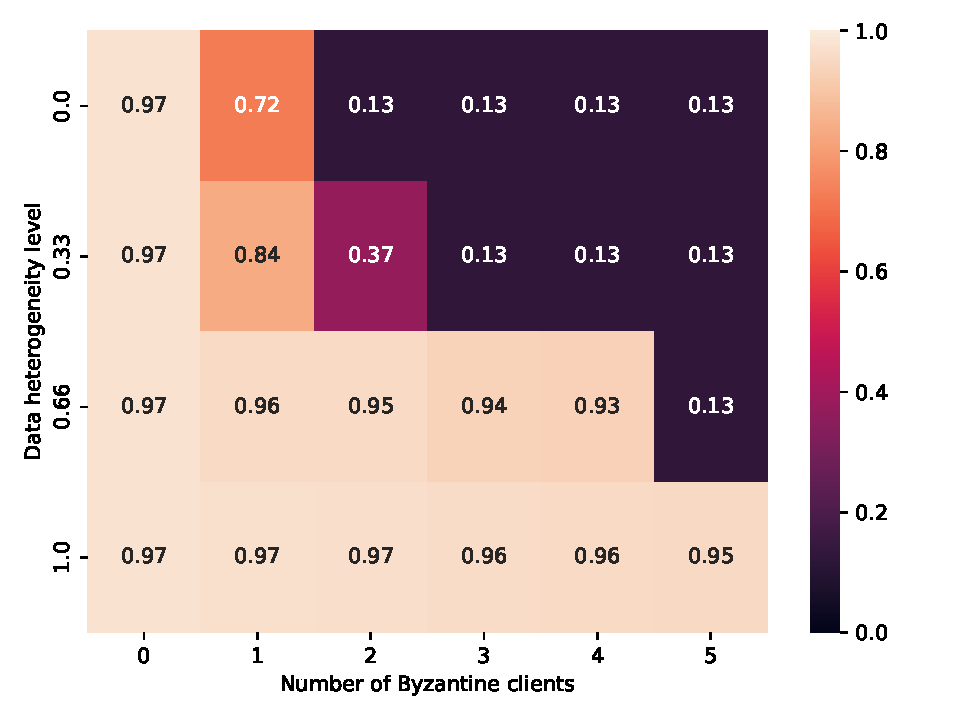
\includegraphics[width=\textwidth]{../plots/robust_new_atan_sweep/alpha_1.5/test_mnist_cnn_mnist_snn_gamma_similarity_niid_NNM_ARC_GeometricMedian_nb_honest_clients_10_tolerated_f_equal_real.pdf}
        \caption{$\alpha = 1.5$}
        \label{fig:gm_worst_case_alpha_1_5}
    \end{subfigure}
    \hfill
    \begin{subfigure}[b]{0.24\textwidth}
        \centering
        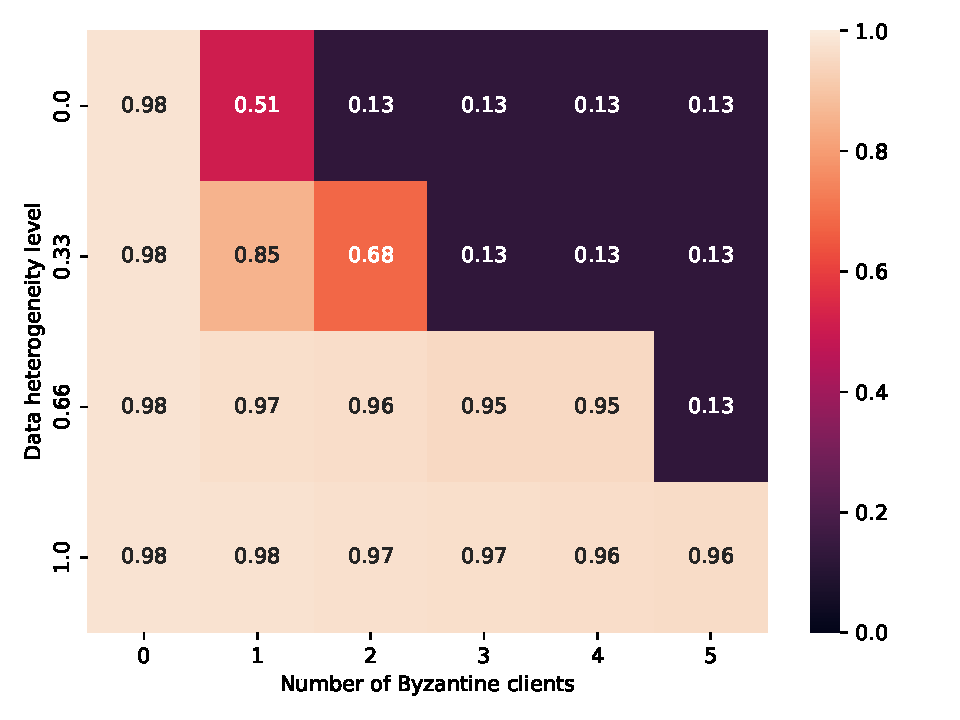
\includegraphics[width=\textwidth]{../plots/robust_new_atan_sweep/alpha_2.0/test_mnist_cnn_mnist_snn_gamma_similarity_niid_NNM_ARC_GeometricMedian_nb_honest_clients_10_tolerated_f_equal_real.pdf}
        \caption{$\alpha = 2.0$}
        \label{fig:gm_worst_case_alpha_2_0}
    \end{subfigure}
    \caption{Geometric Median performance under the worst-case across all attacks across $\alpha$ values.}
    \label{fig:gm_worst_case_grid}
\end{figure}\clearpage
\subsubsection{GM under Optimal ALIE Attack}
\begin{figure}[htbp]
    \centering
    \begin{subfigure}[b]{0.24\textwidth}
        \centering
        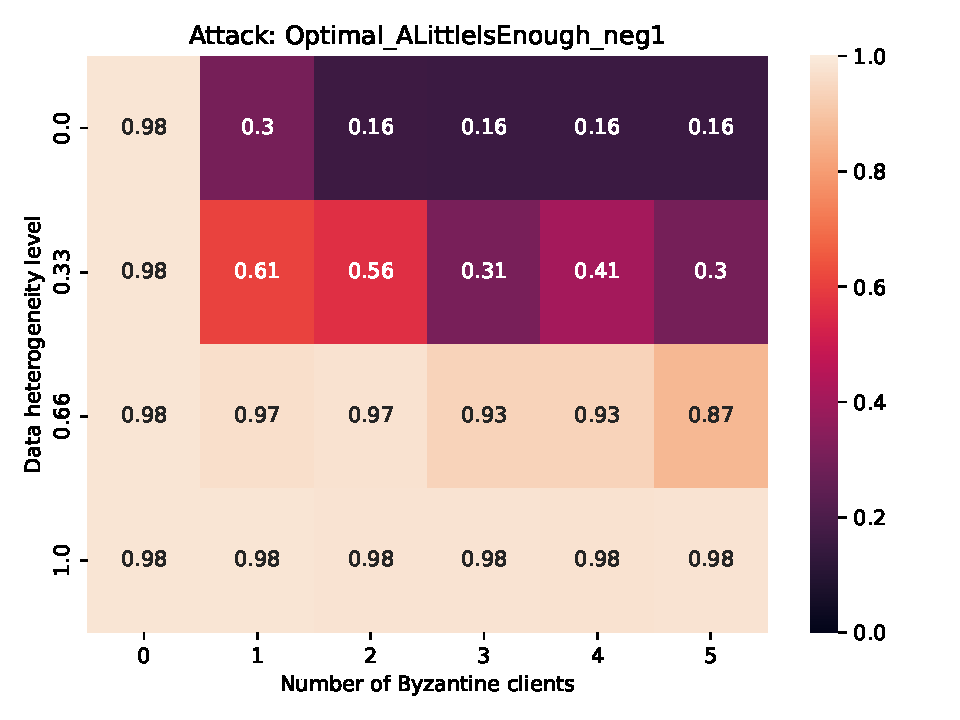
\includegraphics[width=\textwidth]{../plots/robust_comparison_sweep/test_Optimal_ALittleIsEnough_neg1_mnist_cnn_mnist_gamma_similarity_niid_NNM_ARC_GeometricMedian_nb_honest_clients_10_tolerated_f_equal_real.pdf}
        \caption{CNN Baseline}
        \label{fig:gm_alie_cnn}
    \end{subfigure}
    \hfill
    \begin{subfigure}[b]{0.24\textwidth}
        \centering
        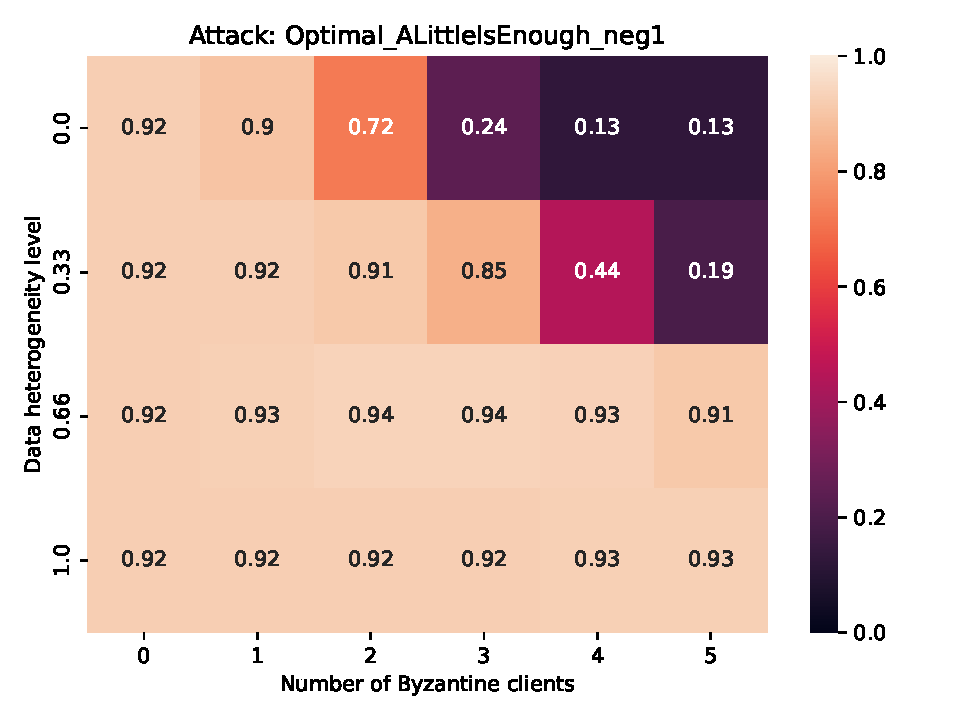
\includegraphics[width=\textwidth]{../plots/robust_new_atan_sweep/alpha_0.5/test_Optimal_ALittleIsEnough_neg1_mnist_cnn_mnist_snn_gamma_similarity_niid_NNM_ARC_GeometricMedian_nb_honest_clients_10_tolerated_f_equal_real.pdf}
        \caption{$\alpha = 0.5$}
        \label{fig:gm_alie_alpha_0_5}
    \end{subfigure}
    \hfill
    \begin{subfigure}[b]{0.24\textwidth}
        \centering
        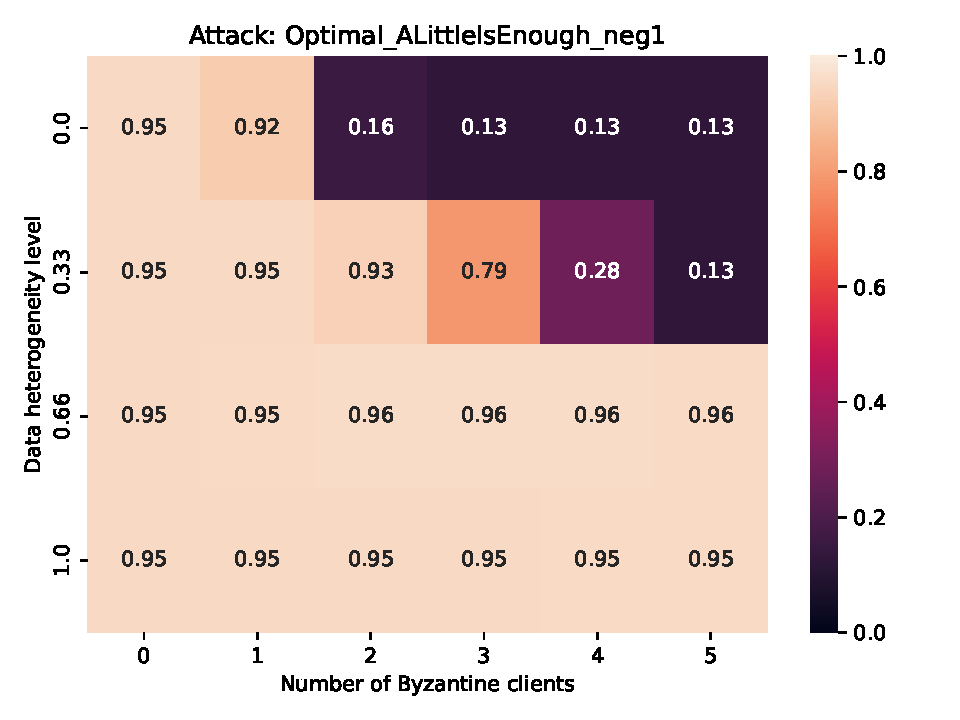
\includegraphics[width=\textwidth]{../plots/robust_new_atan_sweep/alpha_0.75/test_Optimal_ALittleIsEnough_neg1_mnist_cnn_mnist_snn_gamma_similarity_niid_NNM_ARC_GeometricMedian_nb_honest_clients_10_tolerated_f_equal_real.pdf}
        \caption{$\alpha = 0.75$}
        \label{fig:gm_alie_alpha_0_75}
    \end{subfigure}
    \hfill
    \begin{subfigure}[b]{0.24\textwidth}
        \centering
        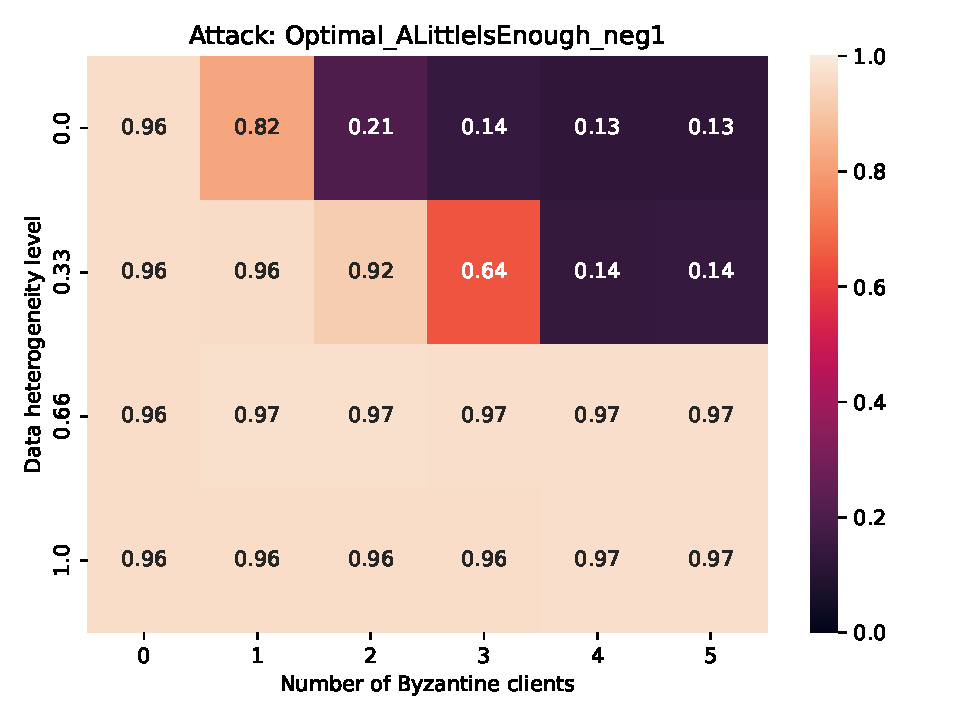
\includegraphics[width=\textwidth]{../plots/robust_new_atan_sweep/alpha_1.0/test_Optimal_ALittleIsEnough_neg1_mnist_cnn_mnist_snn_gamma_similarity_niid_NNM_ARC_GeometricMedian_nb_honest_clients_10_tolerated_f_equal_real.pdf}
        \caption{$\alpha = 1.0$}
        \label{fig:gm_alie_alpha_1_0}
    \end{subfigure}
    \vspace{0.2cm}
    \begin{subfigure}[b]{0.24\textwidth}
        \centering
        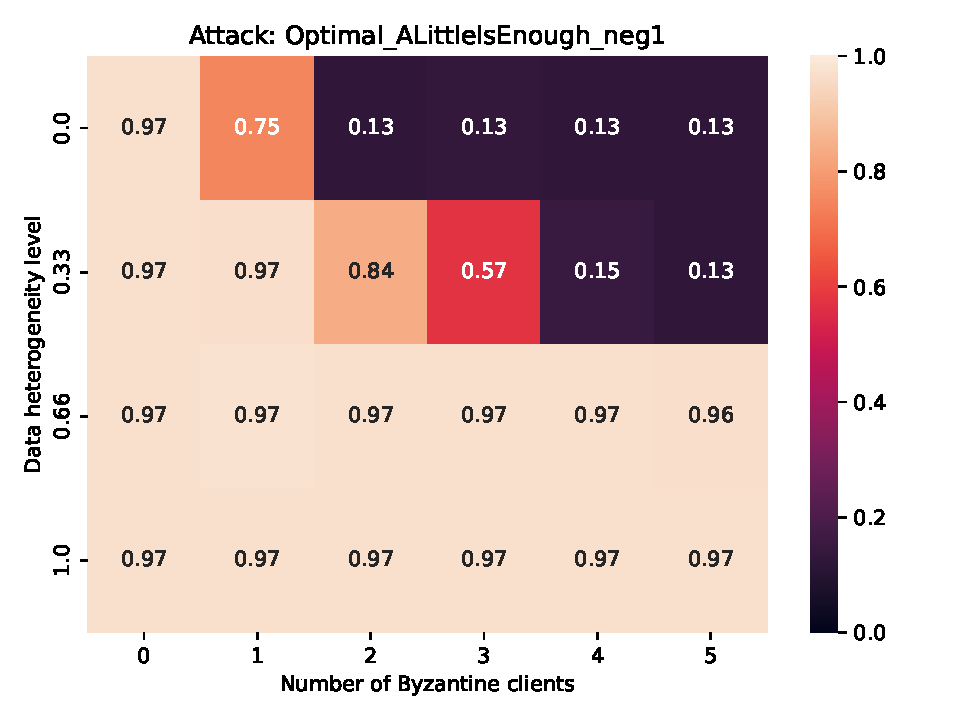
\includegraphics[width=\textwidth]{../plots/robust_new_atan_sweep/alpha_1.2/test_Optimal_ALittleIsEnough_neg1_mnist_cnn_mnist_snn_gamma_similarity_niid_NNM_ARC_GeometricMedian_nb_honest_clients_10_tolerated_f_equal_real.pdf}
        \caption{$\alpha = 1.2$}
        \label{fig:gm_alie_alpha_1_2}
    \end{subfigure}
    \hfill
    \begin{subfigure}[b]{0.24\textwidth}
        \centering
        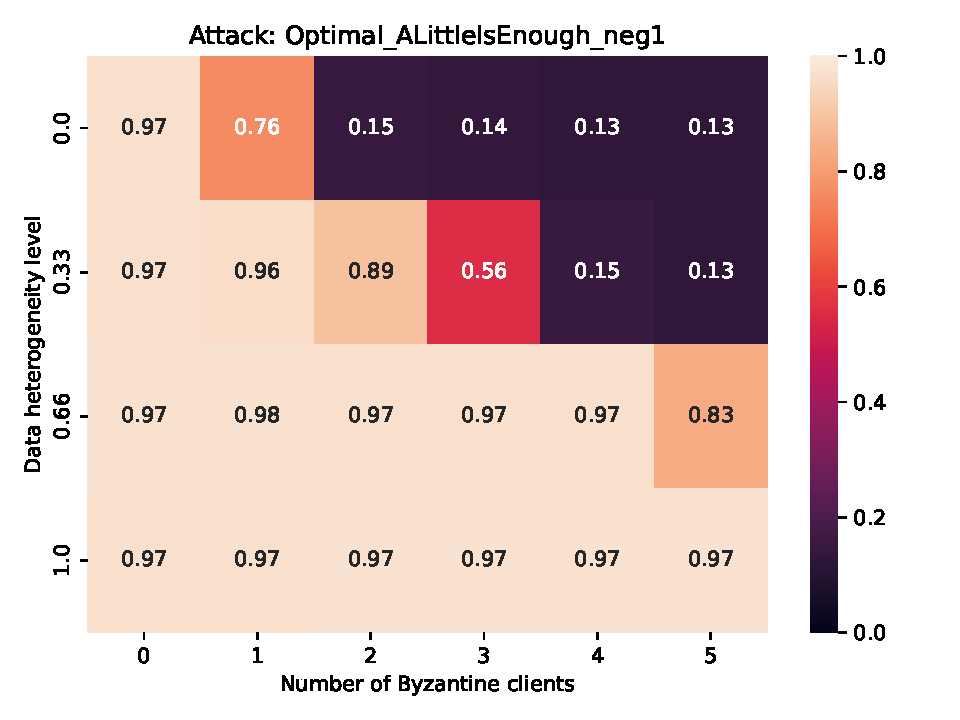
\includegraphics[width=\textwidth]{../plots/robust_new_atan_sweep/alpha_1.4/test_Optimal_ALittleIsEnough_neg1_mnist_cnn_mnist_snn_gamma_similarity_niid_NNM_ARC_GeometricMedian_nb_honest_clients_10_tolerated_f_equal_real.pdf}
        \caption{$\alpha = 1.4$}
        \label{fig:gm_alie_alpha_1_4}
    \end{subfigure}
    \hfill
    \begin{subfigure}[b]{0.24\textwidth}
        \centering
        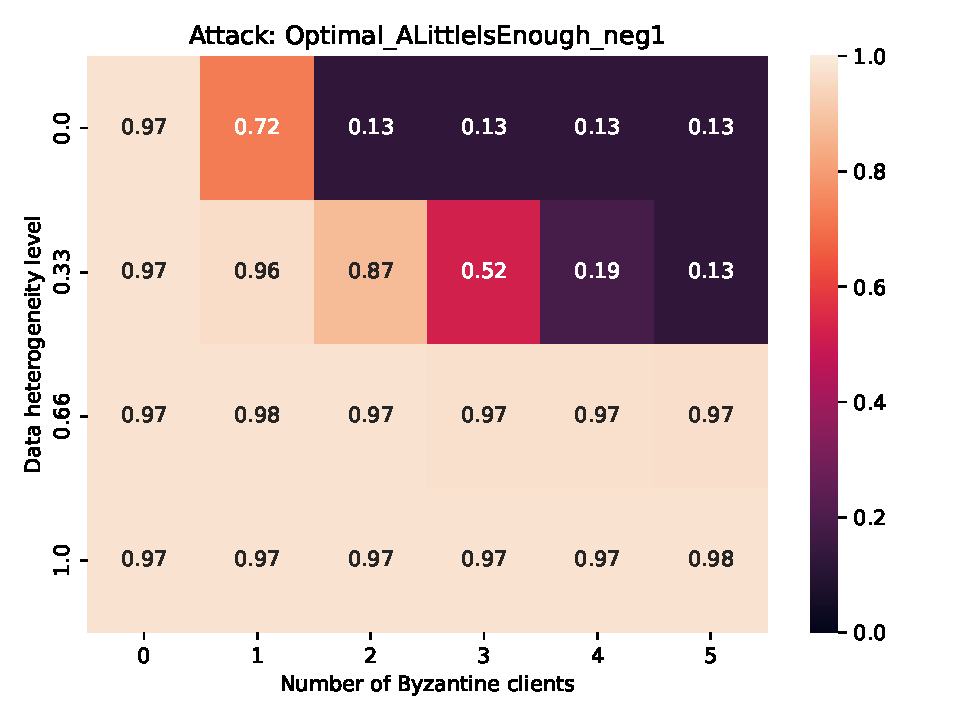
\includegraphics[width=\textwidth]{../plots/robust_new_atan_sweep/alpha_1.5/test_Optimal_ALittleIsEnough_neg1_mnist_cnn_mnist_snn_gamma_similarity_niid_NNM_ARC_GeometricMedian_nb_honest_clients_10_tolerated_f_equal_real.pdf}
        \caption{$\alpha = 1.5$}
        \label{fig:gm_alie_alpha_1_5}
    \end{subfigure}
    \hfill
    \begin{subfigure}[b]{0.24\textwidth}
        \centering
        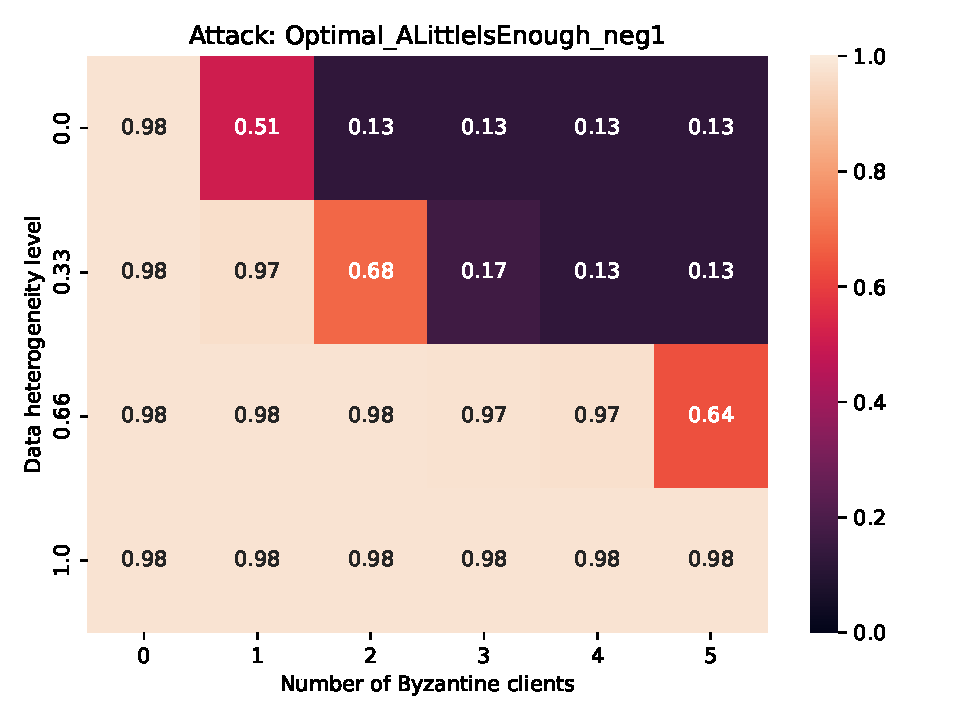
\includegraphics[width=\textwidth]{../plots/robust_new_atan_sweep/alpha_2.0/test_Optimal_ALittleIsEnough_neg1_mnist_cnn_mnist_snn_gamma_similarity_niid_NNM_ARC_GeometricMedian_nb_honest_clients_10_tolerated_f_equal_real.pdf}
        \caption{$\alpha = 2.0$}
        \label{fig:gm_alie_alpha_2_0}
    \end{subfigure}
    \caption{Geometric Median performance under Optimal ALIE across $\alpha$ values.}
    \label{fig:gm_alie_grid}
\end{figure}\clearpage
\subsubsection{GM under Sign Flipping Attack}
\begin{figure}[htbp]
    \centering
    \begin{subfigure}[b]{0.24\textwidth}
        \centering
        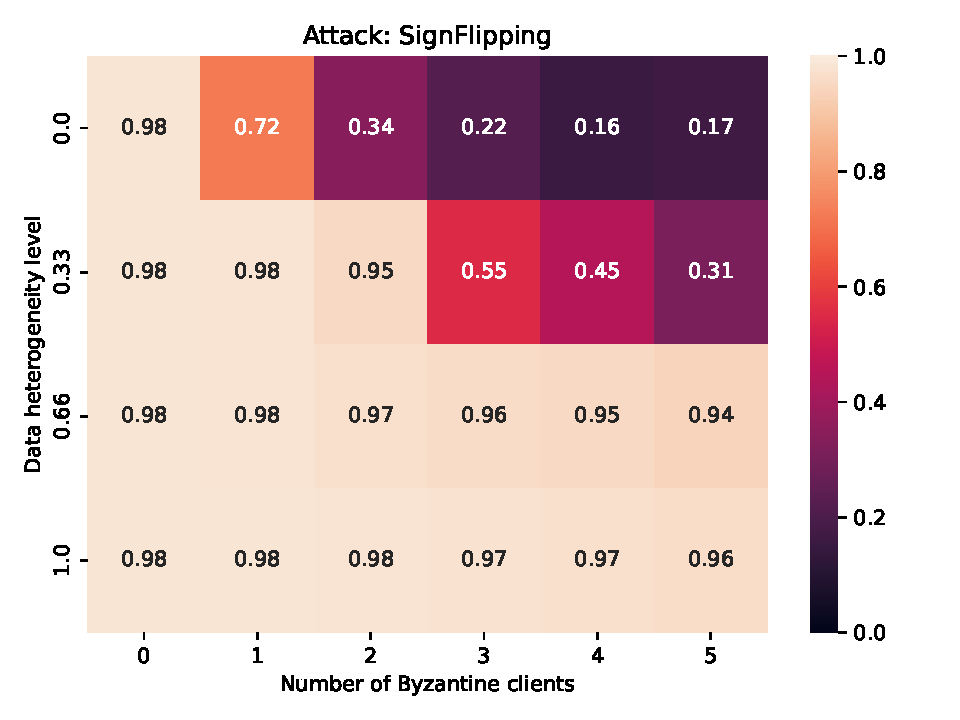
\includegraphics[width=\textwidth]{../plots/robust_comparison_sweep/test_SignFlipping_mnist_cnn_mnist_gamma_similarity_niid_NNM_ARC_GeometricMedian_nb_honest_clients_10_tolerated_f_equal_real.pdf}
        \caption{CNN Baseline}
        \label{fig:gm_sf_cnn}
    \end{subfigure}
    \hfill
    \begin{subfigure}[b]{0.24\textwidth}
        \centering
        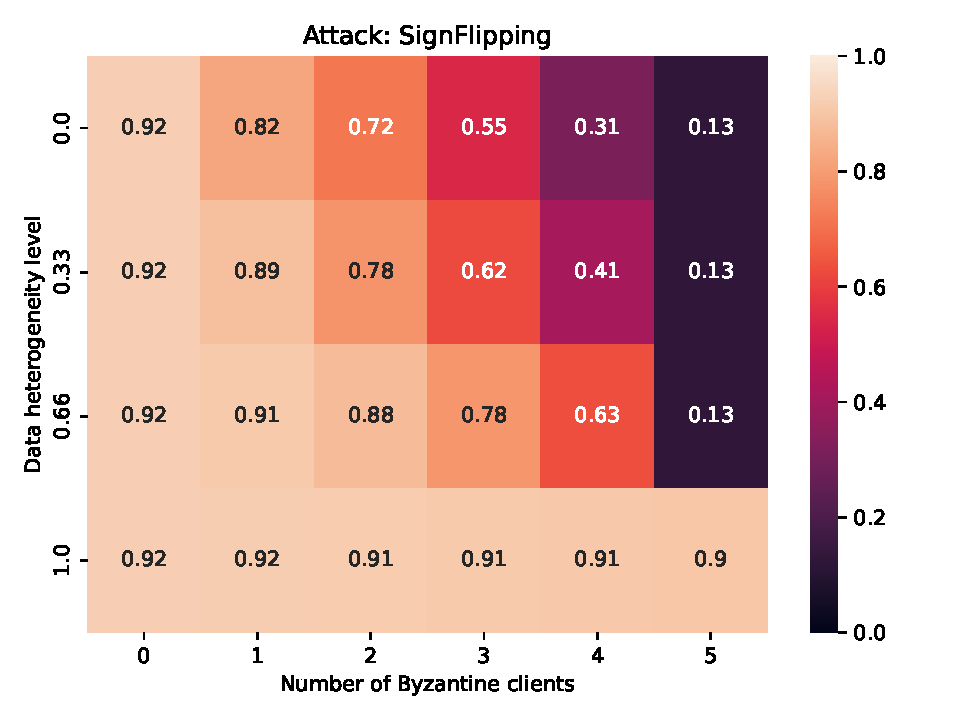
\includegraphics[width=\textwidth]{../plots/robust_new_atan_sweep/alpha_0.5/test_SignFlipping_mnist_cnn_mnist_snn_gamma_similarity_niid_NNM_ARC_GeometricMedian_nb_honest_clients_10_tolerated_f_equal_real.pdf}
        \caption{$\alpha = 0.5$}
        \label{fig:gm_sf_alpha_0_5}
    \end{subfigure}
    \hfill
    \begin{subfigure}[b]{0.24\textwidth}
        \centering
        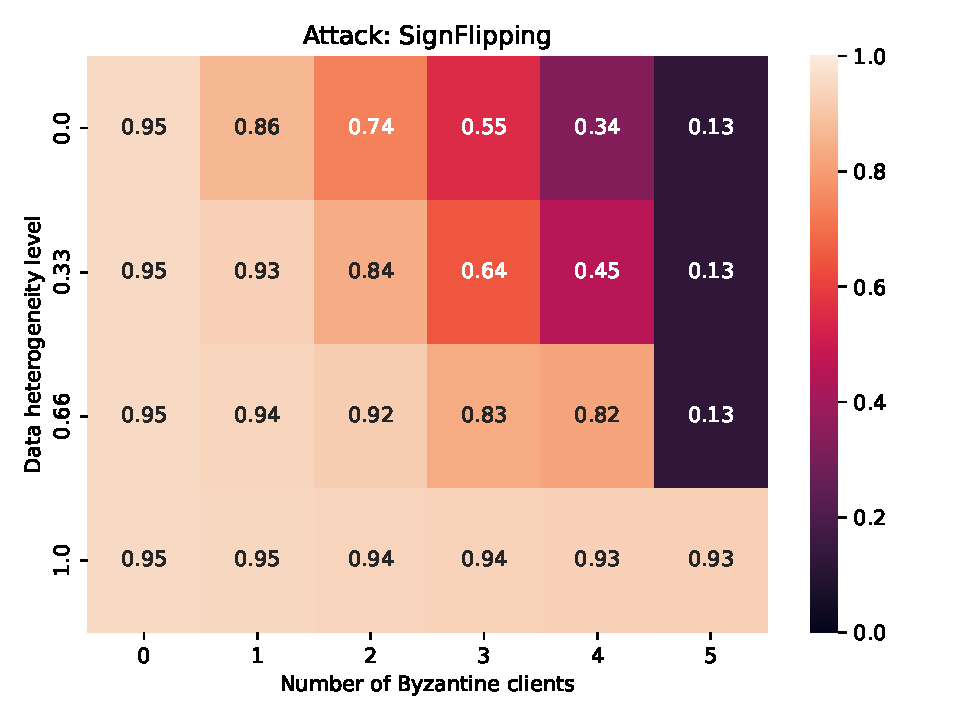
\includegraphics[width=\textwidth]{../plots/robust_new_atan_sweep/alpha_0.75/test_SignFlipping_mnist_cnn_mnist_snn_gamma_similarity_niid_NNM_ARC_GeometricMedian_nb_honest_clients_10_tolerated_f_equal_real.pdf}
        \caption{$\alpha = 0.75$}
        \label{fig:gm_sf_alpha_0_75}
    \end{subfigure}
    \hfill
    \begin{subfigure}[b]{0.24\textwidth}
        \centering
        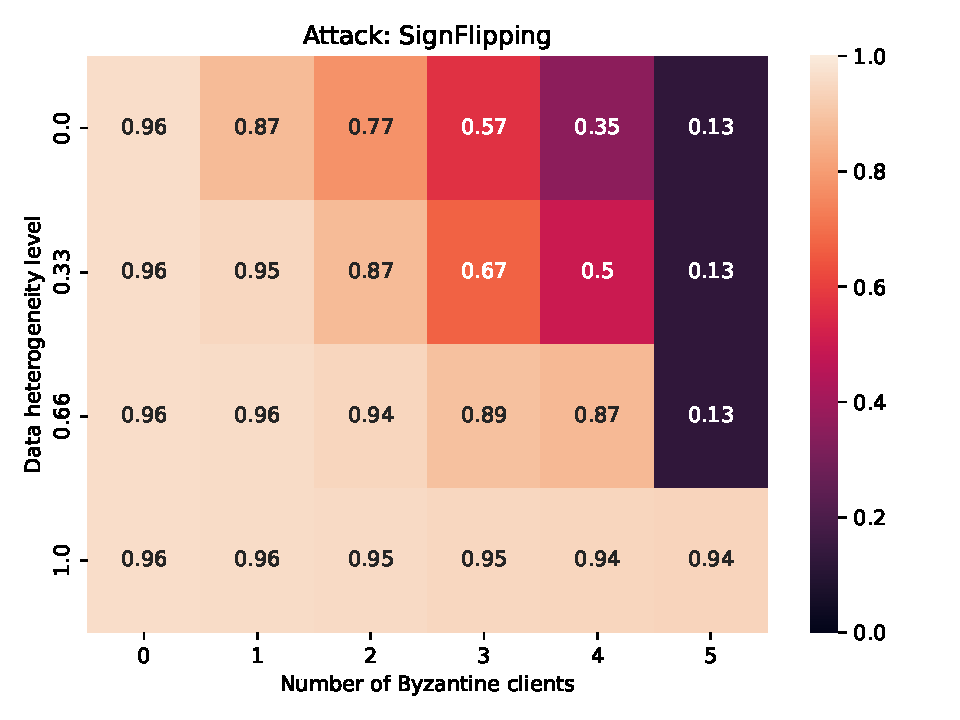
\includegraphics[width=\textwidth]{../plots/robust_new_atan_sweep/alpha_1.0/test_SignFlipping_mnist_cnn_mnist_snn_gamma_similarity_niid_NNM_ARC_GeometricMedian_nb_honest_clients_10_tolerated_f_equal_real.pdf}
        \caption{$\alpha = 1.0$}
        \label{fig:gm_sf_alpha_1_0}
    \end{subfigure}
    \vspace{0.2cm}
    \begin{subfigure}[b]{0.24\textwidth}
        \centering
        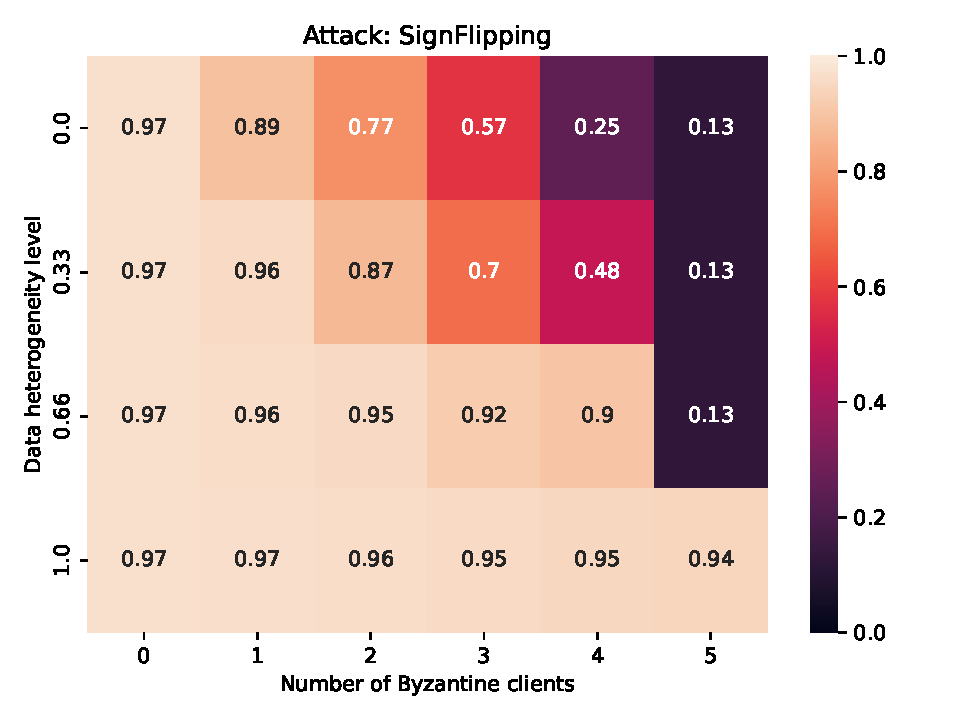
\includegraphics[width=\textwidth]{../plots/robust_new_atan_sweep/alpha_1.2/test_SignFlipping_mnist_cnn_mnist_snn_gamma_similarity_niid_NNM_ARC_GeometricMedian_nb_honest_clients_10_tolerated_f_equal_real.pdf}
        \caption{$\alpha = 1.2$}
        \label{fig:gm_sf_alpha_1_2}
    \end{subfigure}
    \hfill
    \begin{subfigure}[b]{0.24\textwidth}
        \centering
        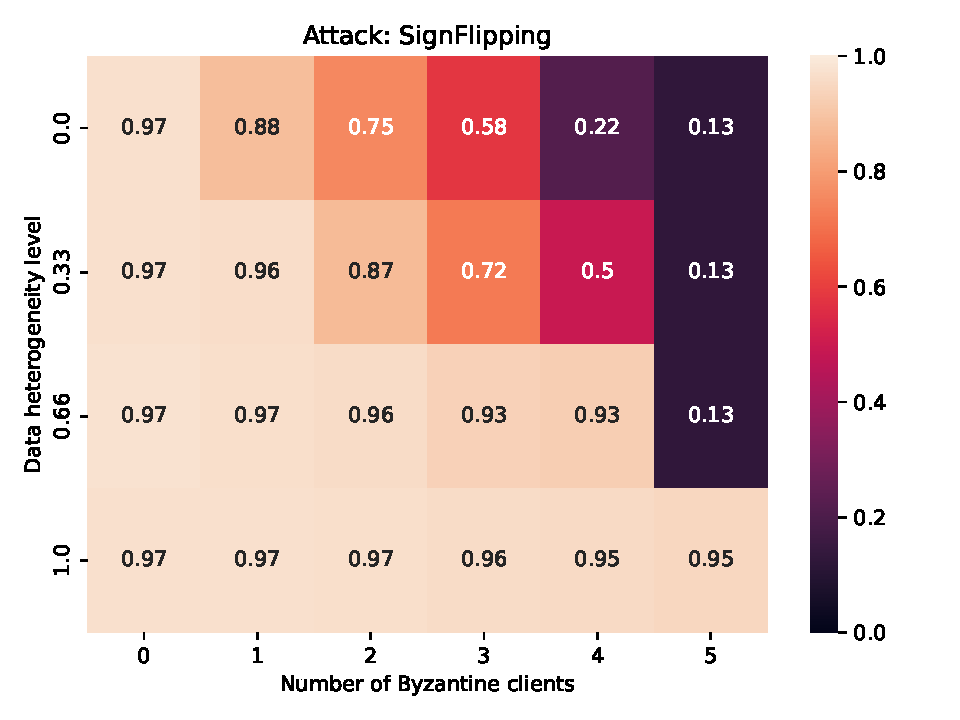
\includegraphics[width=\textwidth]{../plots/robust_new_atan_sweep/alpha_1.4/test_SignFlipping_mnist_cnn_mnist_snn_gamma_similarity_niid_NNM_ARC_GeometricMedian_nb_honest_clients_10_tolerated_f_equal_real.pdf}
        \caption{$\alpha = 1.4$}
        \label{fig:gm_sf_alpha_1_4}
    \end{subfigure}
    \hfill
    \begin{subfigure}[b]{0.24\textwidth}
        \centering
        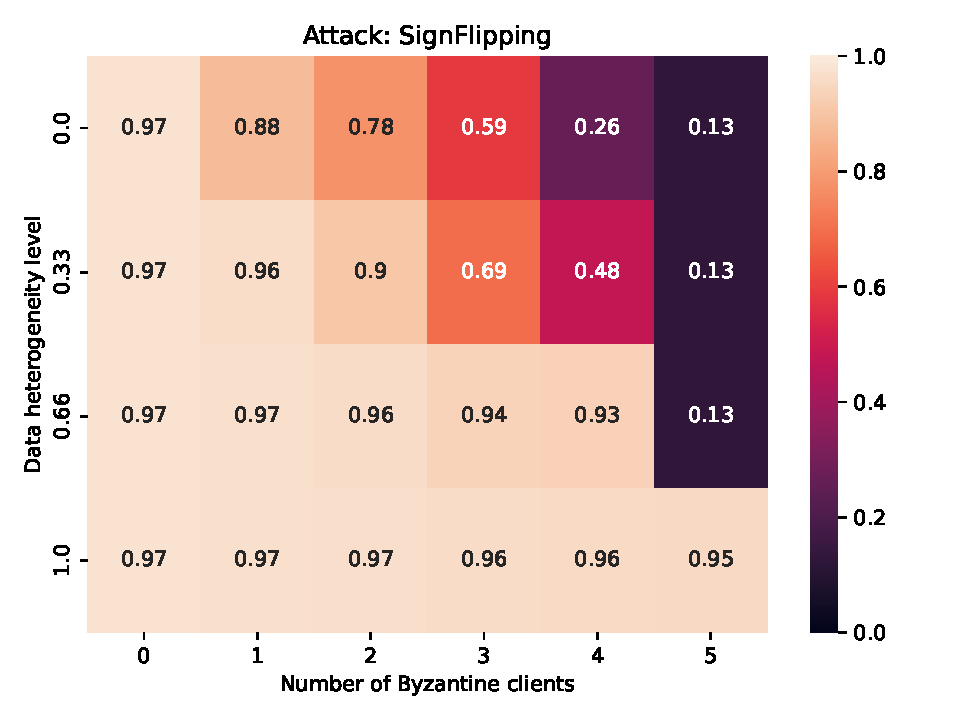
\includegraphics[width=\textwidth]{../plots/robust_new_atan_sweep/alpha_1.5/test_SignFlipping_mnist_cnn_mnist_snn_gamma_similarity_niid_NNM_ARC_GeometricMedian_nb_honest_clients_10_tolerated_f_equal_real.pdf}
        \caption{$\alpha = 1.5$}
        \label{fig:gm_sf_alpha_1_5}
    \end{subfigure}
    \hfill
    \begin{subfigure}[b]{0.24\textwidth}
        \centering
        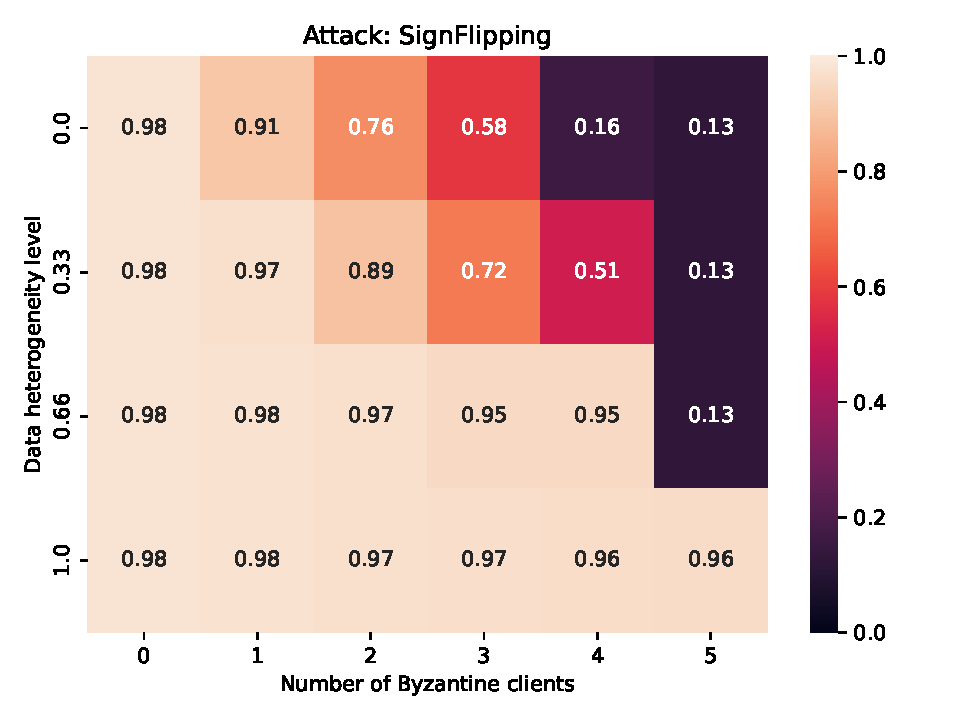
\includegraphics[width=\textwidth]{../plots/robust_new_atan_sweep/alpha_2.0/test_SignFlipping_mnist_cnn_mnist_snn_gamma_similarity_niid_NNM_ARC_GeometricMedian_nb_honest_clients_10_tolerated_f_equal_real.pdf}
        \caption{$\alpha = 2.0$}
        \label{fig:gm_sf_alpha_2_0}
    \end{subfigure}
    \caption{Geometric Median performance under Sign Flipping across $\alpha$ values.}
    \label{fig:gm_sf_grid}
\end{figure}\clearpage
\subsubsection{GM under Optimal Inner Product Manipulation Attack}
\begin{figure}[htbp]
    \centering
    \begin{subfigure}[b]{0.24\textwidth}
        \centering
        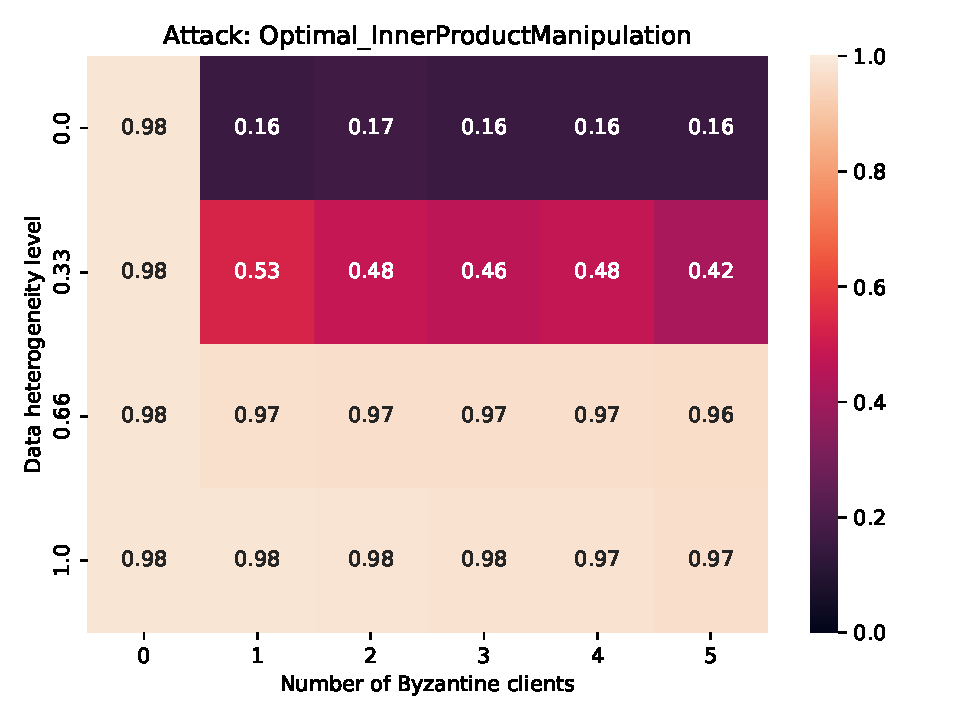
\includegraphics[width=\textwidth]{../plots/robust_comparison_sweep/test_Optimal_InnerProductManipulation_mnist_cnn_mnist_gamma_similarity_niid_NNM_ARC_GeometricMedian_nb_honest_clients_10_tolerated_f_equal_real.pdf}
        \caption{CNN Baseline}
        \label{fig:gm_ipm_cnn}
    \end{subfigure}
    \hfill
    \begin{subfigure}[b]{0.24\textwidth}
        \centering
        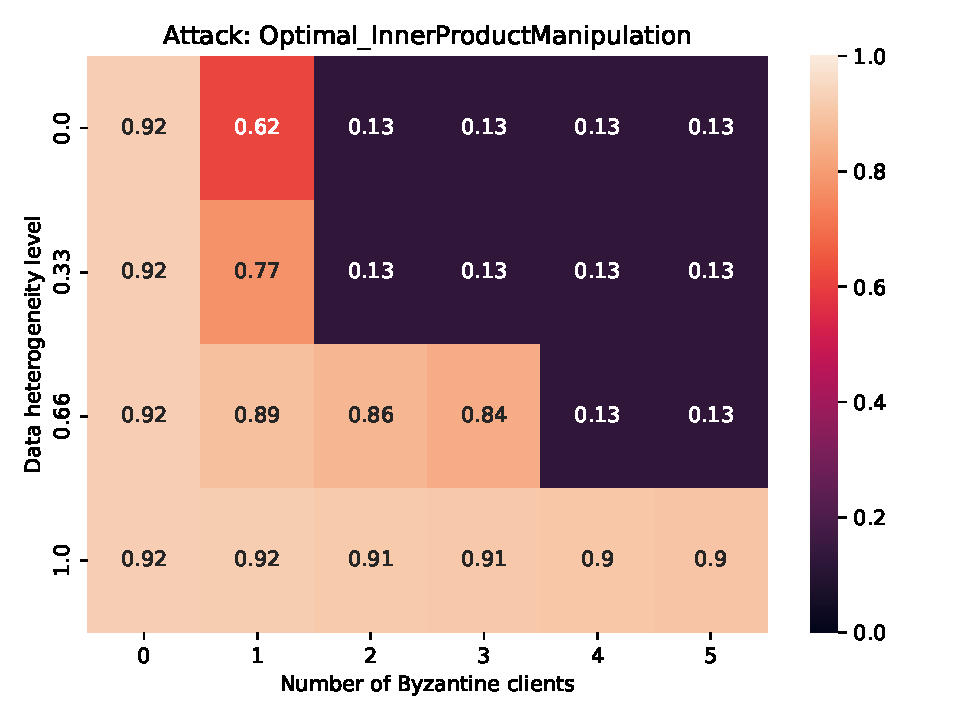
\includegraphics[width=\textwidth]{../plots/robust_new_atan_sweep/alpha_0.5/test_Optimal_InnerProductManipulation_mnist_cnn_mnist_snn_gamma_similarity_niid_NNM_ARC_GeometricMedian_nb_honest_clients_10_tolerated_f_equal_real.pdf}
        \caption{$\alpha = 0.5$}
        \label{fig:gm_ipm_alpha_0_5}
    \end{subfigure}
    \hfill
    \begin{subfigure}[b]{0.24\textwidth}
        \centering
        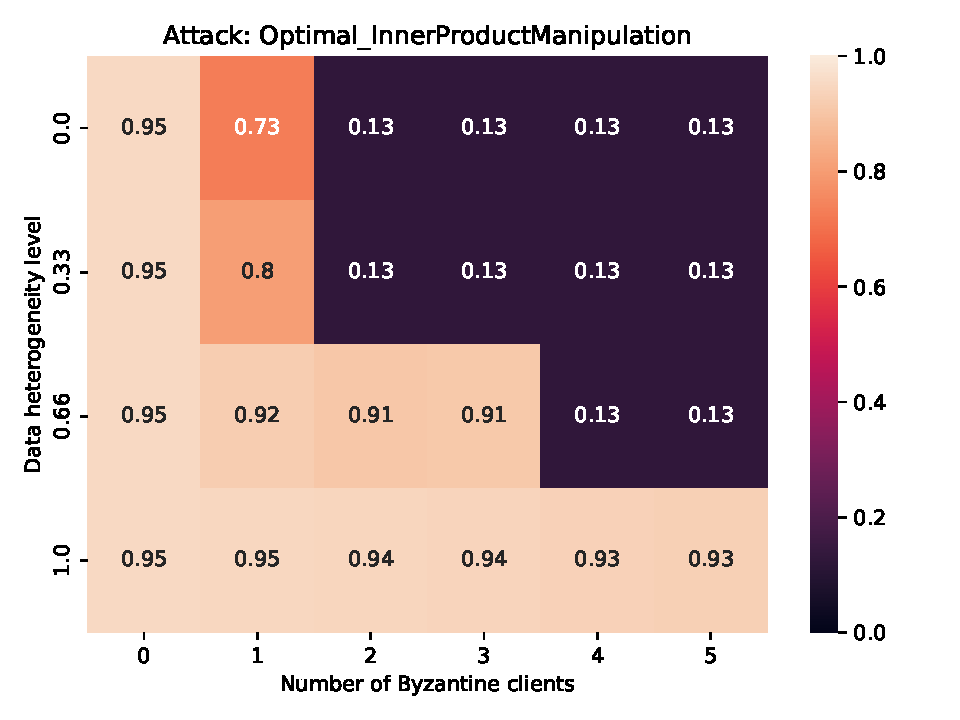
\includegraphics[width=\textwidth]{../plots/robust_new_atan_sweep/alpha_0.75/test_Optimal_InnerProductManipulation_mnist_cnn_mnist_snn_gamma_similarity_niid_NNM_ARC_GeometricMedian_nb_honest_clients_10_tolerated_f_equal_real.pdf}
        \caption{$\alpha = 0.75$}
        \label{fig:gm_ipm_alpha_0_75}
    \end{subfigure}
    \hfill
    \begin{subfigure}[b]{0.24\textwidth}
        \centering
        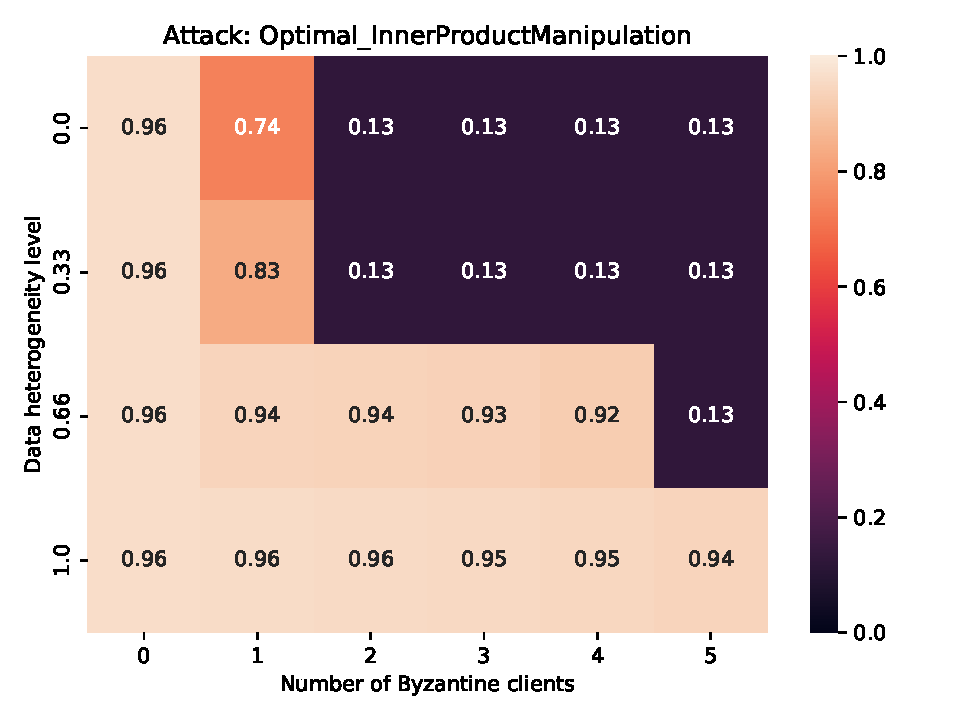
\includegraphics[width=\textwidth]{../plots/robust_new_atan_sweep/alpha_1.0/test_Optimal_InnerProductManipulation_mnist_cnn_mnist_snn_gamma_similarity_niid_NNM_ARC_GeometricMedian_nb_honest_clients_10_tolerated_f_equal_real.pdf}
        \caption{$\alpha = 1.0$}
        \label{fig:gm_ipm_alpha_1_0}
    \end{subfigure}
    \vspace{0.2cm}
    \begin{subfigure}[b]{0.24\textwidth}
        \centering
        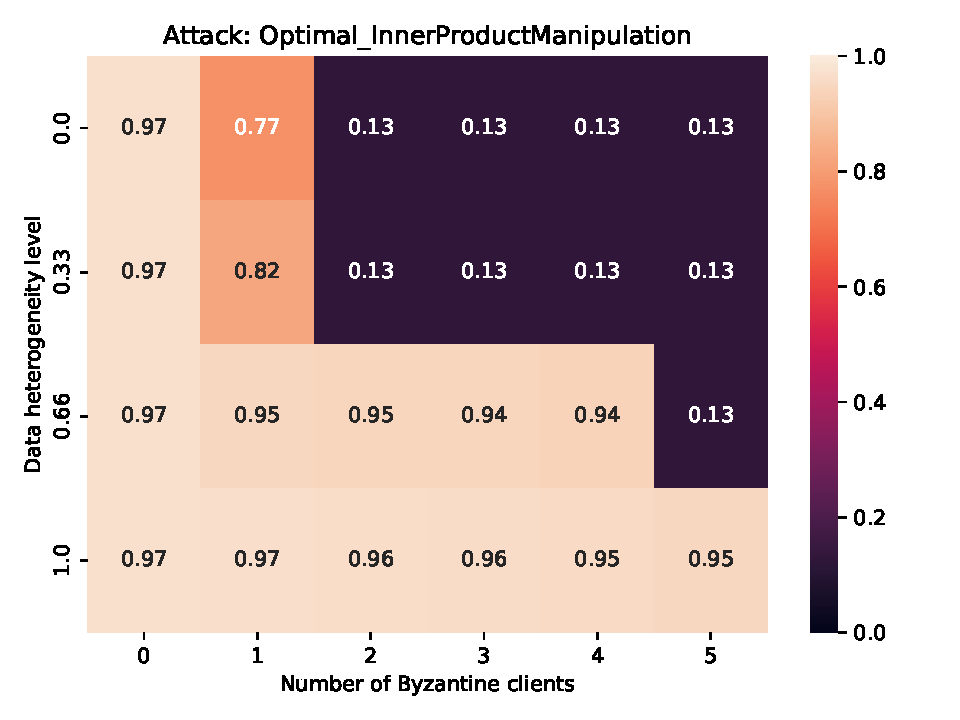
\includegraphics[width=\textwidth]{../plots/robust_new_atan_sweep/alpha_1.2/test_Optimal_InnerProductManipulation_mnist_cnn_mnist_snn_gamma_similarity_niid_NNM_ARC_GeometricMedian_nb_honest_clients_10_tolerated_f_equal_real.pdf}
        \caption{$\alpha = 1.2$}
        \label{fig:gm_ipm_alpha_1_2}
    \end{subfigure}
    \hfill
    \begin{subfigure}[b]{0.24\textwidth}
        \centering
        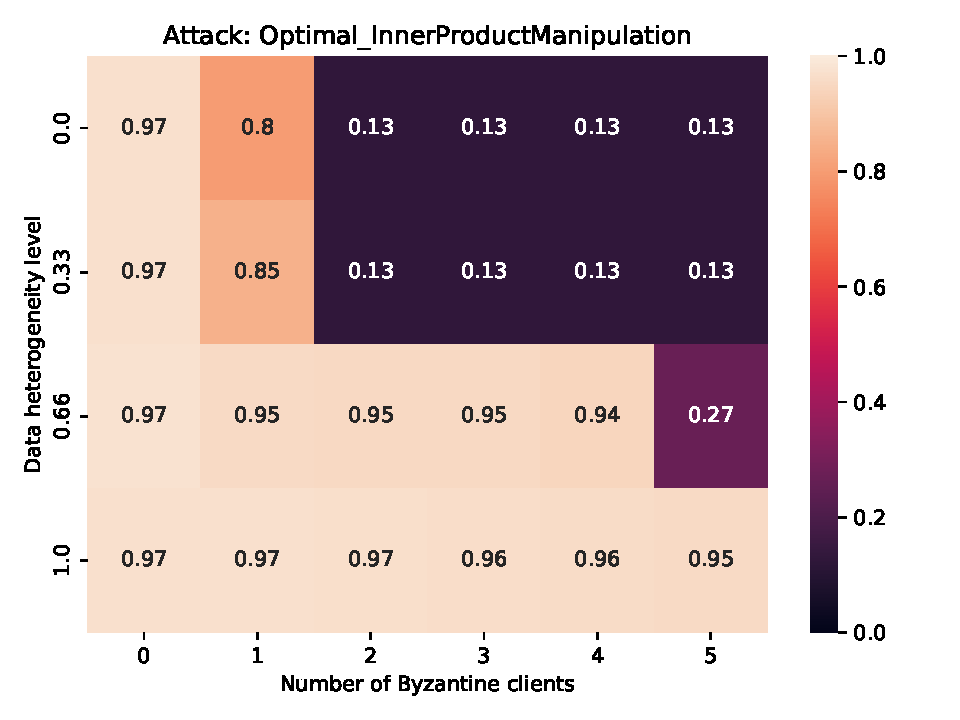
\includegraphics[width=\textwidth]{../plots/robust_new_atan_sweep/alpha_1.4/test_Optimal_InnerProductManipulation_mnist_cnn_mnist_snn_gamma_similarity_niid_NNM_ARC_GeometricMedian_nb_honest_clients_10_tolerated_f_equal_real.pdf}
        \caption{$\alpha = 1.4$}
        \label{fig:gm_ipm_alpha_1_4}
    \end{subfigure}
    \hfill
    \begin{subfigure}[b]{0.24\textwidth}
        \centering
        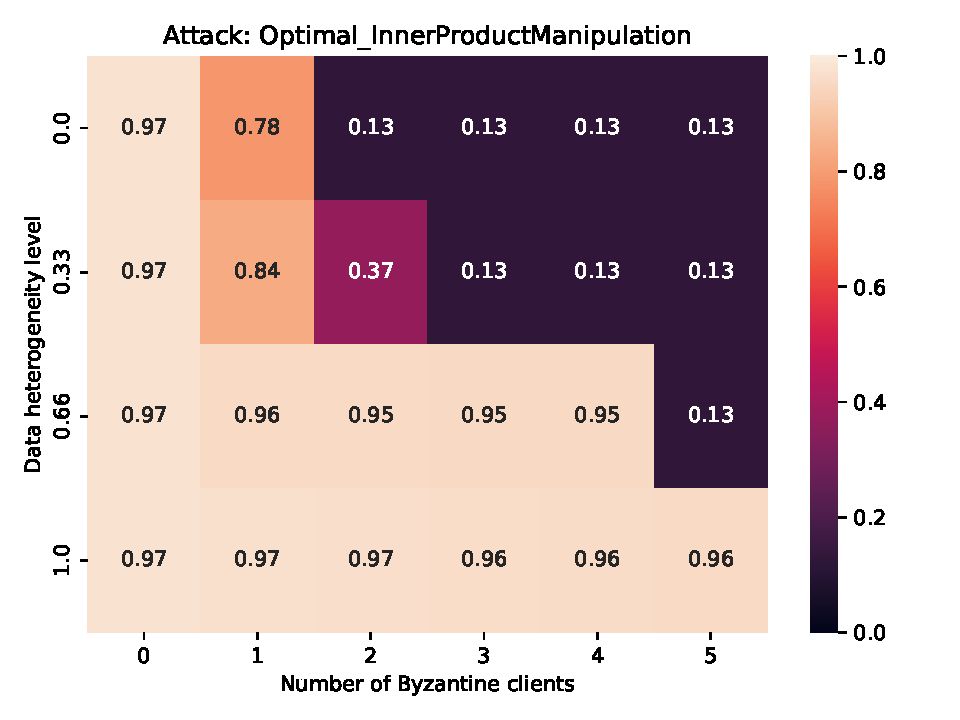
\includegraphics[width=\textwidth]{../plots/robust_new_atan_sweep/alpha_1.5/test_Optimal_InnerProductManipulation_mnist_cnn_mnist_snn_gamma_similarity_niid_NNM_ARC_GeometricMedian_nb_honest_clients_10_tolerated_f_equal_real.pdf}
        \caption{$\alpha = 1.5$}
        \label{fig:gm_ipm_alpha_1_5}
    \end{subfigure}
    \hfill
    \begin{subfigure}[b]{0.24\textwidth}
        \centering
        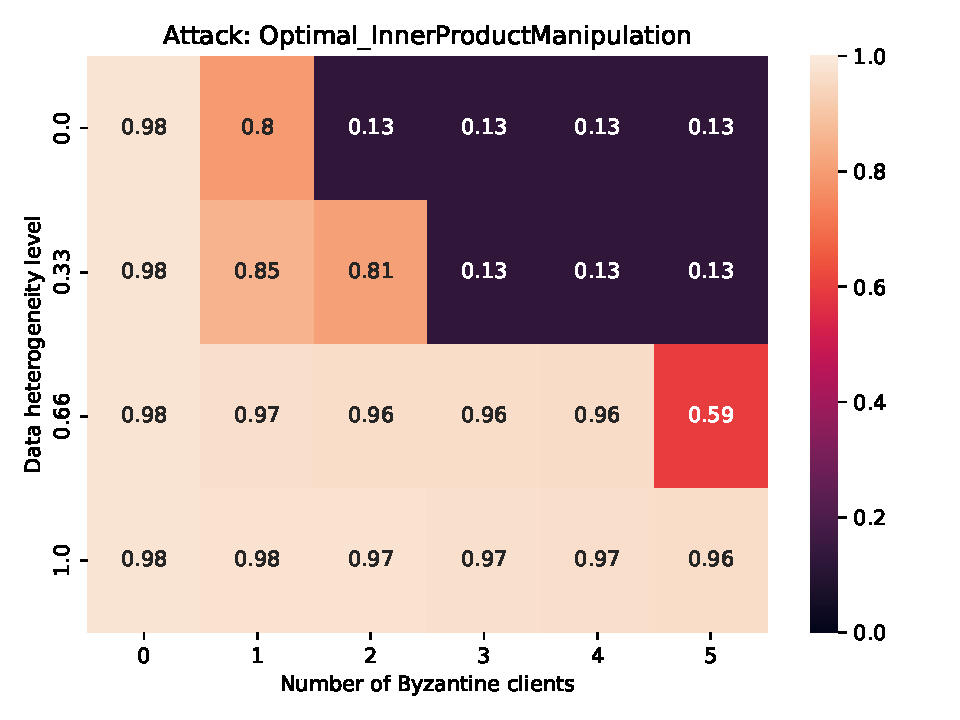
\includegraphics[width=\textwidth]{../plots/robust_new_atan_sweep/alpha_2.0/test_Optimal_InnerProductManipulation_mnist_cnn_mnist_snn_gamma_similarity_niid_NNM_ARC_GeometricMedian_nb_honest_clients_10_tolerated_f_equal_real.pdf}
        \caption{$\alpha = 2.0$}
        \label{fig:gm_ipm_alpha_2_0}
    \end{subfigure}
    \caption{Geometric Median performance under Optimal Inner Product Manipulation across $\alpha$ values.}
    \label{fig:gm_ipm_grid}
\end{figure}
\clearpage
\subsection{Multi-Krum (MK)}
\subsubsection{MK under Worst-Case across all Attacks}
\begin{figure}[htbp]
    \centering
    \begin{subfigure}[b]{0.24\textwidth}
        \centering
        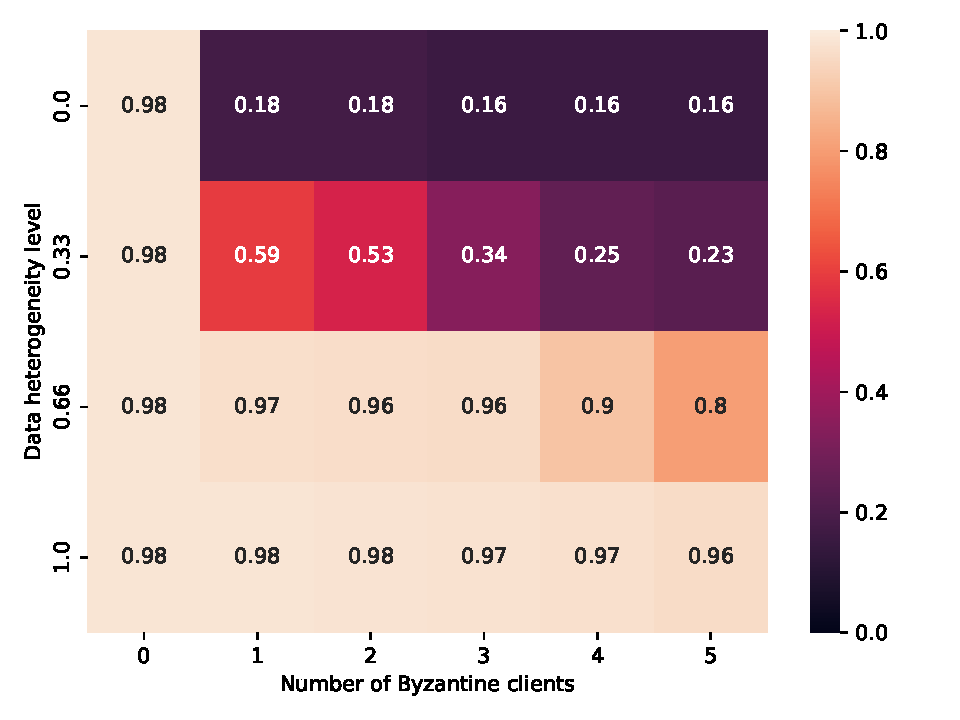
\includegraphics[width=\textwidth]{../plots/robust_comparison_sweep/test_mnist_cnn_mnist_gamma_similarity_niid_NNM_ARC_MultiKrum_nb_honest_clients_10_tolerated_f_equal_real.pdf}
        \caption{CNN Baseline}
        \label{fig:mk_worst_case_cnn}
    \end{subfigure}
    \hfill
    \begin{subfigure}[b]{0.24\textwidth}
        \centering
        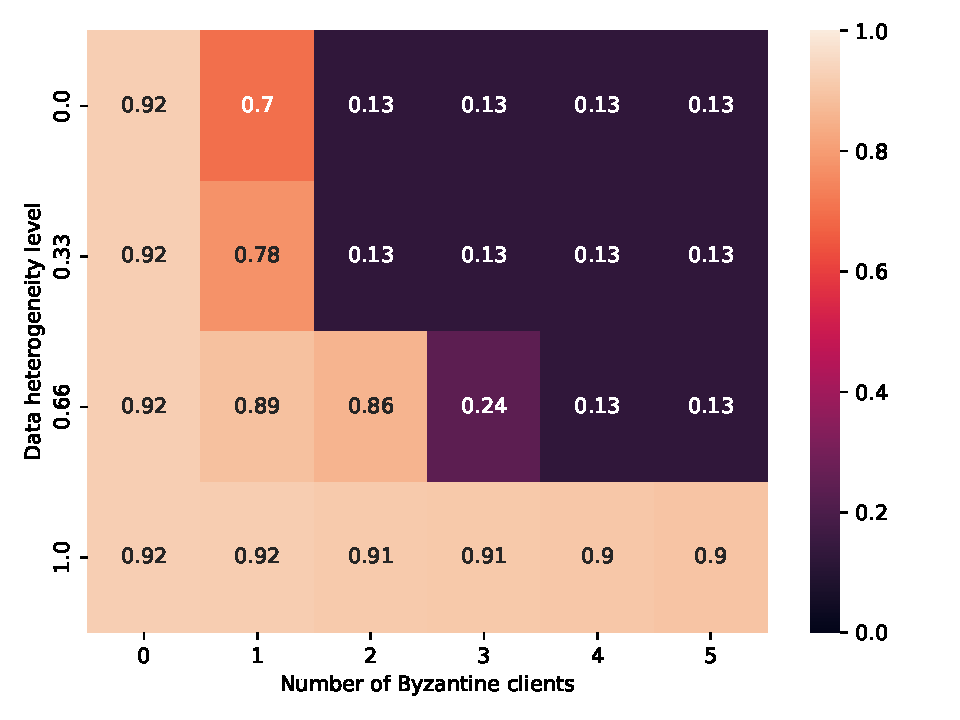
\includegraphics[width=\textwidth]{../plots/robust_new_atan_sweep/alpha_0.5/test_mnist_cnn_mnist_snn_gamma_similarity_niid_NNM_ARC_MultiKrum_nb_honest_clients_10_tolerated_f_equal_real.pdf}
        \caption{$\alpha = 0.5$}
        \label{fig:mk_worst_case_alpha_0_5}
    \end{subfigure}
    \hfill
    \begin{subfigure}[b]{0.24\textwidth}
        \centering
        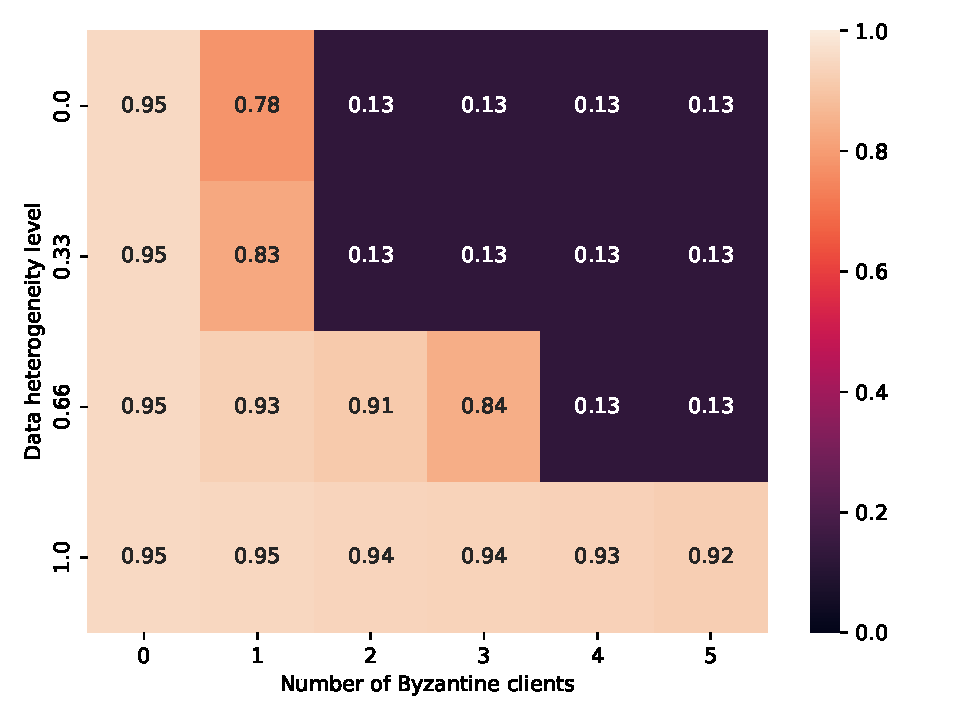
\includegraphics[width=\textwidth]{../plots/robust_new_atan_sweep/alpha_0.75/test_mnist_cnn_mnist_snn_gamma_similarity_niid_NNM_ARC_MultiKrum_nb_honest_clients_10_tolerated_f_equal_real.pdf}
        \caption{$\alpha = 0.75$}
        \label{fig:mk_worst_case_alpha_0_75}
    \end{subfigure}
    \hfill
    \begin{subfigure}[b]{0.24\textwidth}
        \centering
        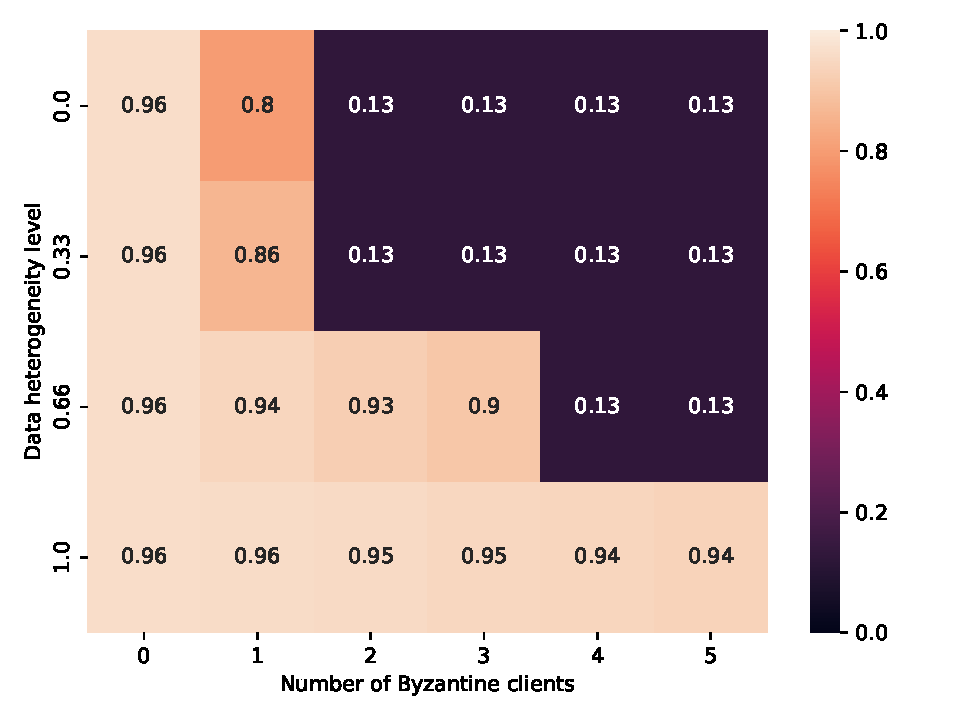
\includegraphics[width=\textwidth]{../plots/robust_new_atan_sweep/alpha_1.0/test_mnist_cnn_mnist_snn_gamma_similarity_niid_NNM_ARC_MultiKrum_nb_honest_clients_10_tolerated_f_equal_real.pdf}
        \caption{$\alpha = 1.0$}
        \label{fig:mk_worst_case_alpha_1_0}
    \end{subfigure}
    \vspace{0.2cm}
    \begin{subfigure}[b]{0.24\textwidth}
        \centering
        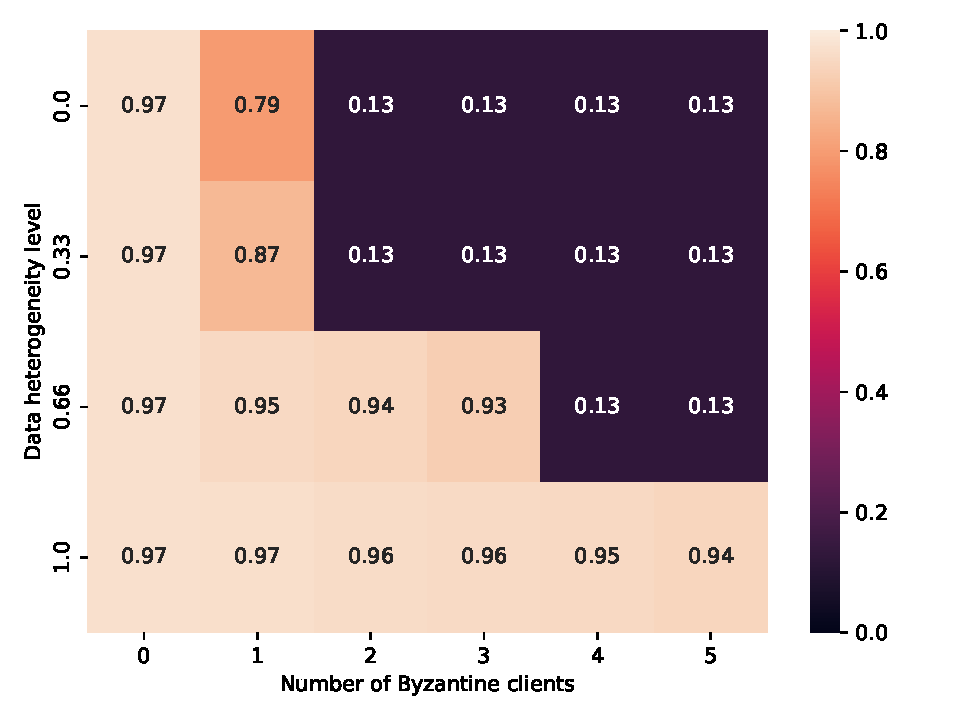
\includegraphics[width=\textwidth]{../plots/robust_new_atan_sweep/alpha_1.2/test_mnist_cnn_mnist_snn_gamma_similarity_niid_NNM_ARC_MultiKrum_nb_honest_clients_10_tolerated_f_equal_real.pdf}
        \caption{$\alpha = 1.2$}
        \label{fig:mk_worst_case_alpha_1_2}
    \end{subfigure}
    \hfill
    \begin{subfigure}[b]{0.24\textwidth}
        \centering
        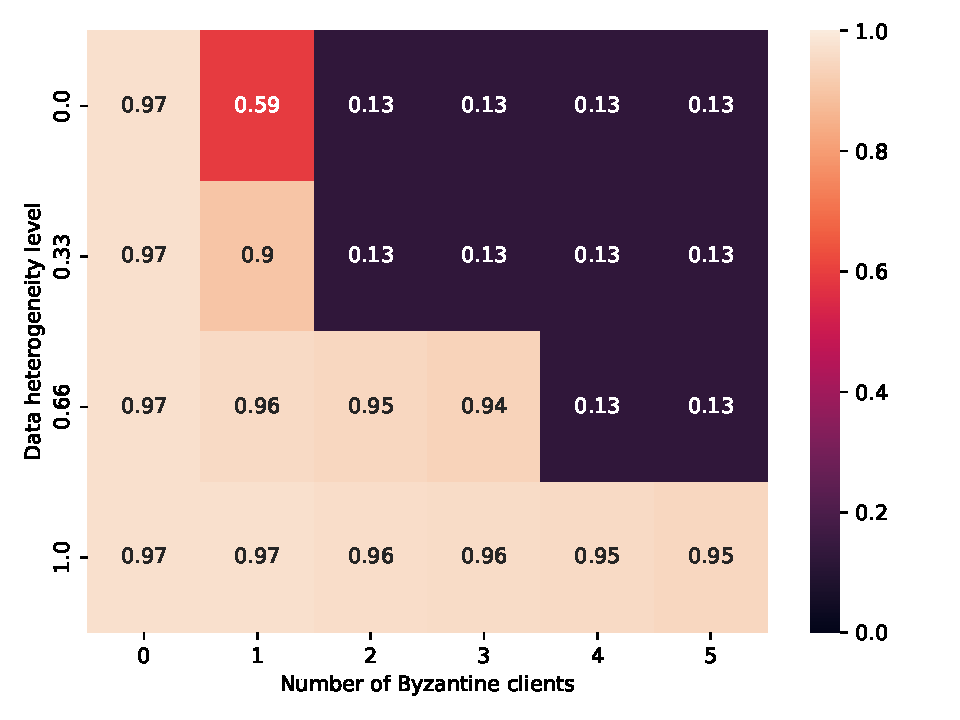
\includegraphics[width=\textwidth]{../plots/robust_new_atan_sweep/alpha_1.4/test_mnist_cnn_mnist_snn_gamma_similarity_niid_NNM_ARC_MultiKrum_nb_honest_clients_10_tolerated_f_equal_real.pdf}
        \caption{$\alpha = 1.4$}
        \label{fig:mk_worst_case_alpha_1_4}
    \end{subfigure}
    \hfill
    \begin{subfigure}[b]{0.24\textwidth}
        \centering
        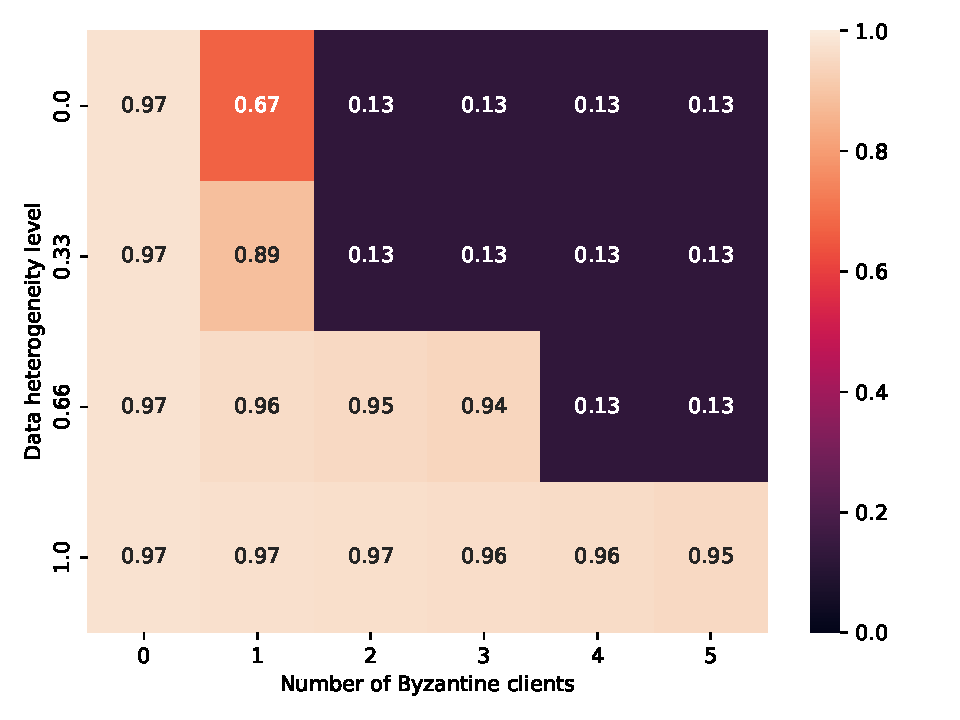
\includegraphics[width=\textwidth]{../plots/robust_new_atan_sweep/alpha_1.5/test_mnist_cnn_mnist_snn_gamma_similarity_niid_NNM_ARC_MultiKrum_nb_honest_clients_10_tolerated_f_equal_real.pdf}
        \caption{$\alpha = 1.5$}
        \label{fig:mk_worst_case_alpha_1_5}
    \end{subfigure}
    \hfill
    \begin{subfigure}[b]{0.24\textwidth}
        \centering
        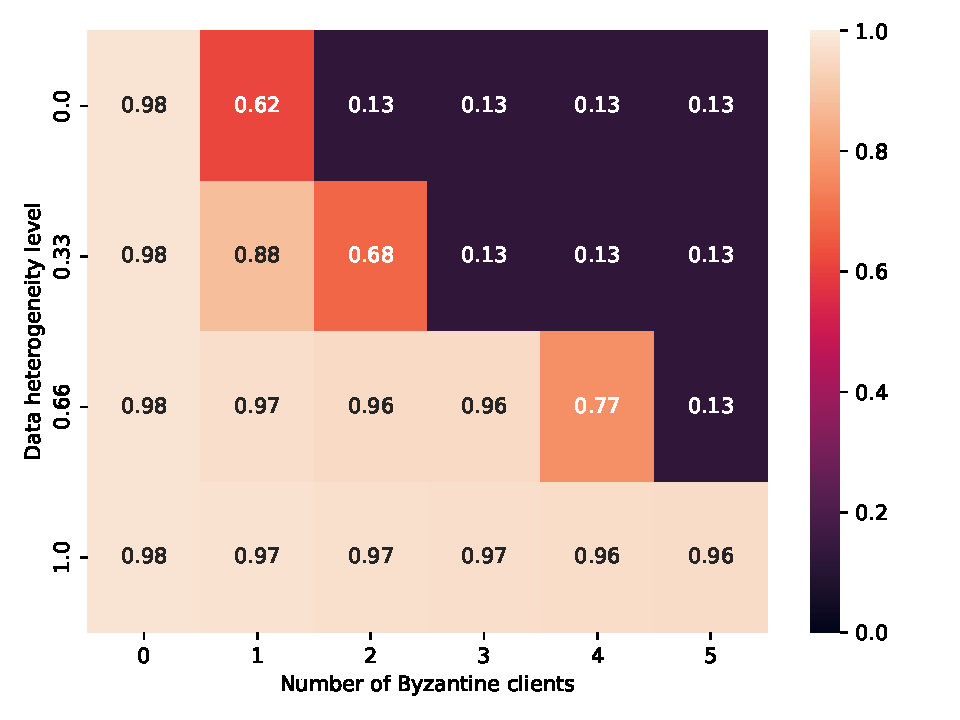
\includegraphics[width=\textwidth]{../plots/robust_new_atan_sweep/alpha_2.0/test_mnist_cnn_mnist_snn_gamma_similarity_niid_NNM_ARC_MultiKrum_nb_honest_clients_10_tolerated_f_equal_real.pdf}
        \caption{$\alpha = 2.0$}
        \label{fig:mk_worst_case_alpha_2_0}
    \end{subfigure}
    \caption{Multi-Krum performance under the worst-case across all attacks across $\alpha$ values.}
    \label{fig:mk_worst_case_grid}
\end{figure}\clearpage
\subsubsection{MK under Optimal ALIE Attack}
\begin{figure}[htbp]
    \centering
    \begin{subfigure}[b]{0.24\textwidth}
        \centering
        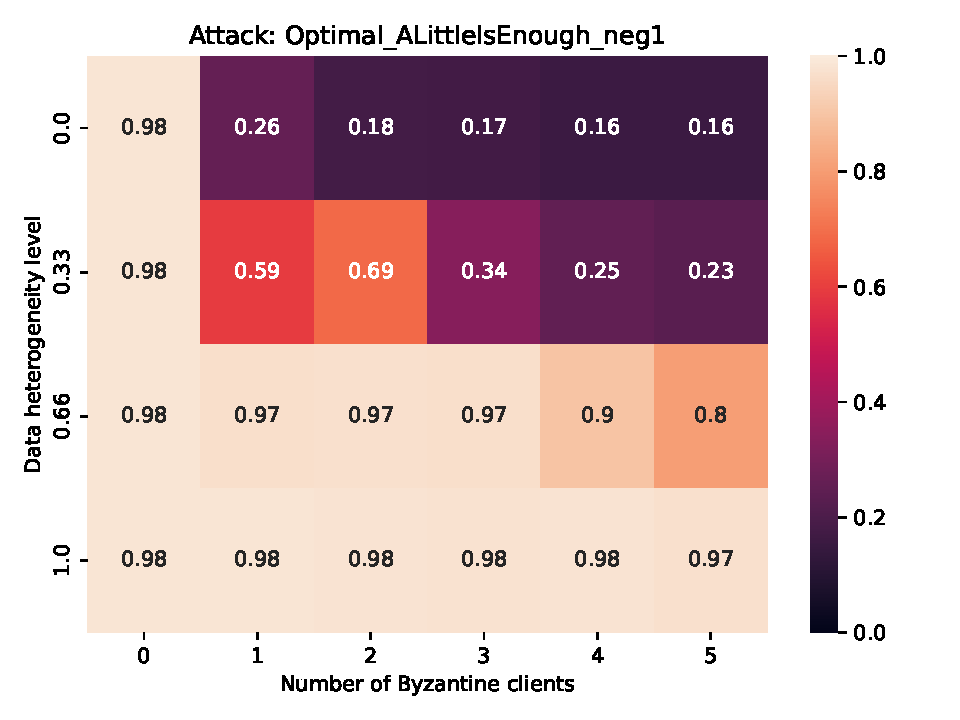
\includegraphics[width=\textwidth]{../plots/robust_comparison_sweep/test_Optimal_ALittleIsEnough_neg1_mnist_cnn_mnist_gamma_similarity_niid_NNM_ARC_MultiKrum_nb_honest_clients_10_tolerated_f_equal_real.pdf}
        \caption{CNN Baseline}
        \label{fig:mk_alie_cnn}
    \end{subfigure}
    \hfill
    \begin{subfigure}[b]{0.24\textwidth}
        \centering
        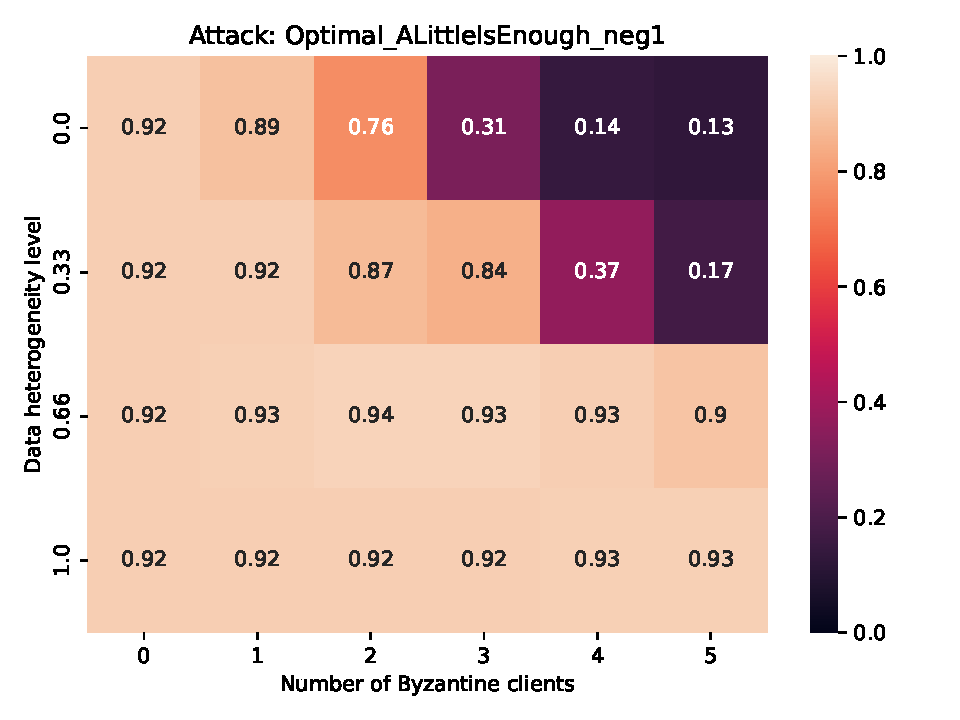
\includegraphics[width=\textwidth]{../plots/robust_new_atan_sweep/alpha_0.5/test_Optimal_ALittleIsEnough_neg1_mnist_cnn_mnist_snn_gamma_similarity_niid_NNM_ARC_MultiKrum_nb_honest_clients_10_tolerated_f_equal_real.pdf}
        \caption{$\alpha = 0.5$}
        \label{fig:mk_alie_alpha_0_5}
    \end{subfigure}
    \hfill
    \begin{subfigure}[b]{0.24\textwidth}
        \centering
        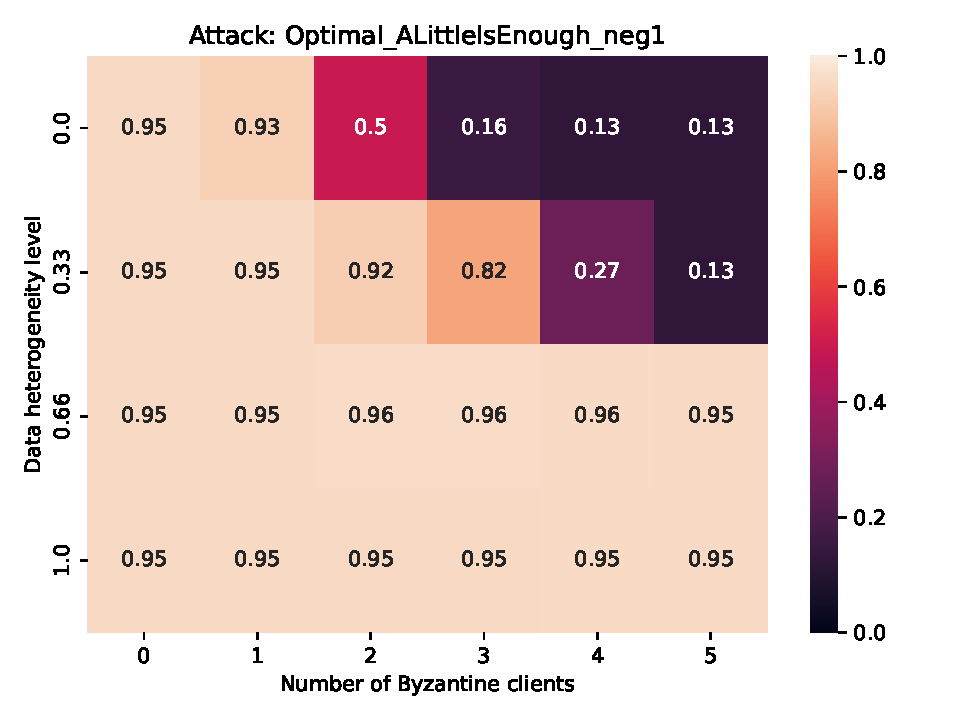
\includegraphics[width=\textwidth]{../plots/robust_new_atan_sweep/alpha_0.75/test_Optimal_ALittleIsEnough_neg1_mnist_cnn_mnist_snn_gamma_similarity_niid_NNM_ARC_MultiKrum_nb_honest_clients_10_tolerated_f_equal_real.pdf}
        \caption{$\alpha = 0.75$}
        \label{fig:mk_alie_alpha_0_75}
    \end{subfigure}
    \hfill
    \begin{subfigure}[b]{0.24\textwidth}
        \centering
        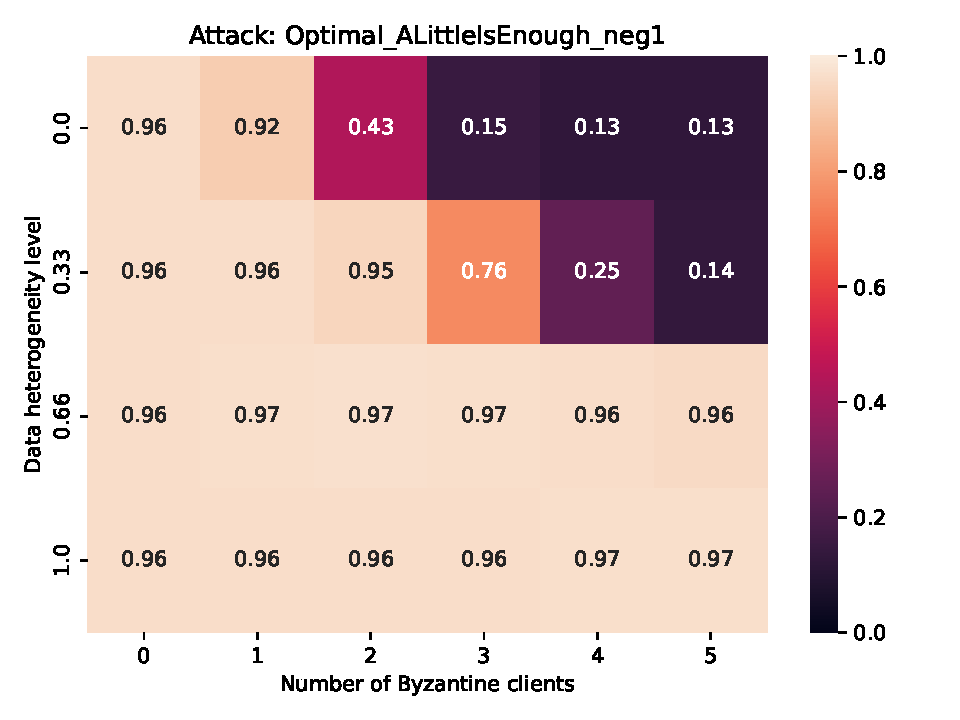
\includegraphics[width=\textwidth]{../plots/robust_new_atan_sweep/alpha_1.0/test_Optimal_ALittleIsEnough_neg1_mnist_cnn_mnist_snn_gamma_similarity_niid_NNM_ARC_MultiKrum_nb_honest_clients_10_tolerated_f_equal_real.pdf}
        \caption{$\alpha = 1.0$}
        \label{fig:mk_alie_alpha_1_0}
    \end{subfigure}
    \vspace{0.2cm}
    \begin{subfigure}[b]{0.24\textwidth}
        \centering
        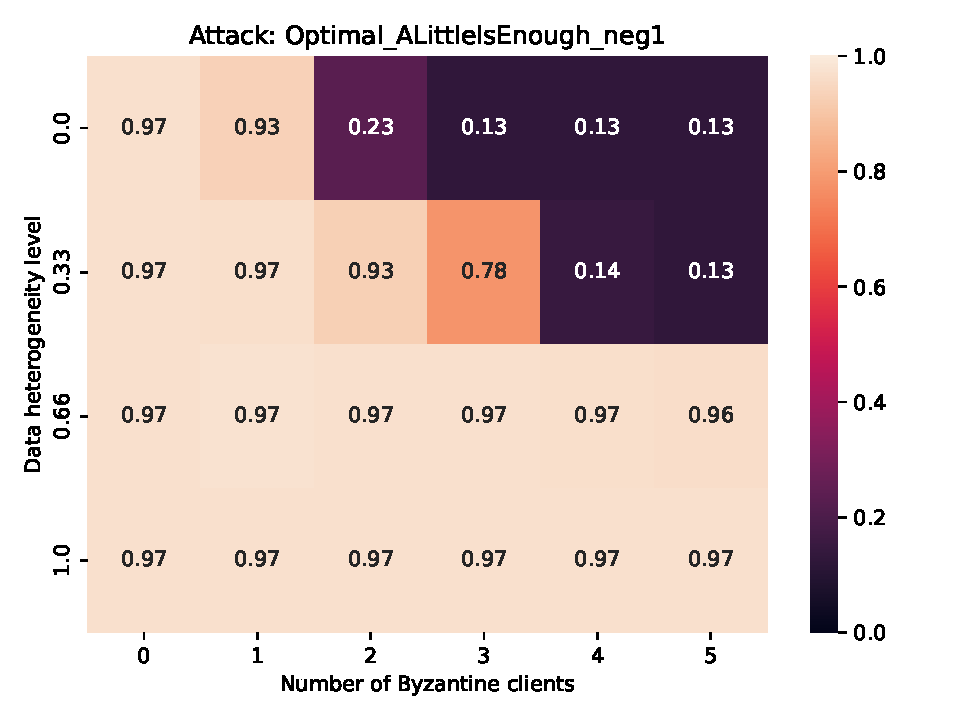
\includegraphics[width=\textwidth]{../plots/robust_new_atan_sweep/alpha_1.2/test_Optimal_ALittleIsEnough_neg1_mnist_cnn_mnist_snn_gamma_similarity_niid_NNM_ARC_MultiKrum_nb_honest_clients_10_tolerated_f_equal_real.pdf}
        \caption{$\alpha = 1.2$}
        \label{fig:mk_alie_alpha_1_2}
    \end{subfigure}
    \hfill
    \begin{subfigure}[b]{0.24\textwidth}
        \centering
        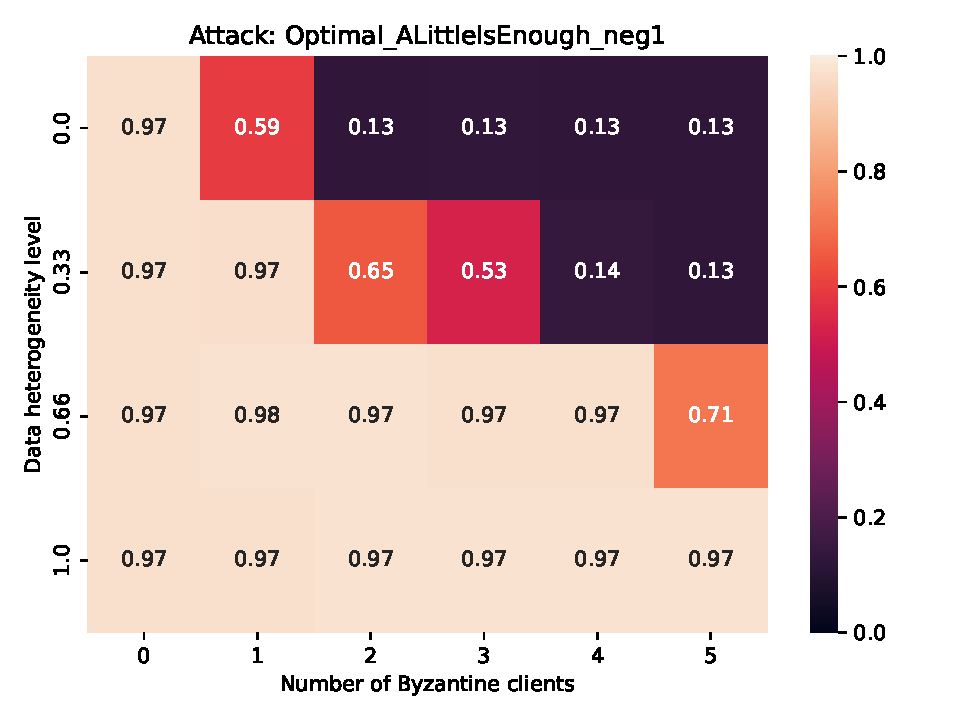
\includegraphics[width=\textwidth]{../plots/robust_new_atan_sweep/alpha_1.4/test_Optimal_ALittleIsEnough_neg1_mnist_cnn_mnist_snn_gamma_similarity_niid_NNM_ARC_MultiKrum_nb_honest_clients_10_tolerated_f_equal_real.pdf}
        \caption{$\alpha = 1.4$}
        \label{fig:mk_alie_alpha_1_4}
    \end{subfigure}
    \hfill
    \begin{subfigure}[b]{0.24\textwidth}
        \centering
        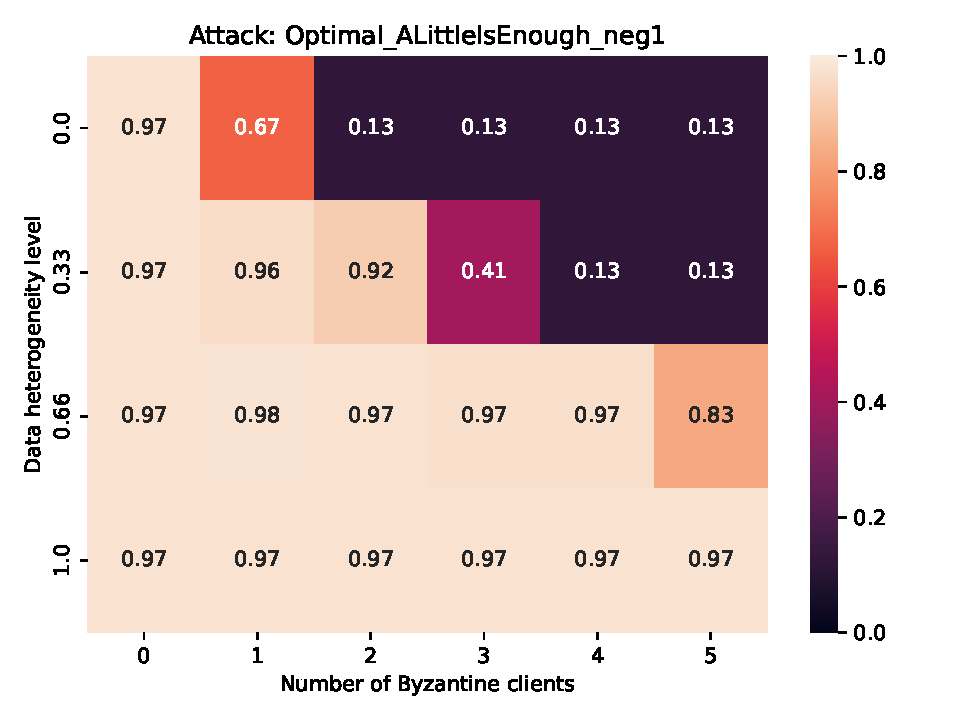
\includegraphics[width=\textwidth]{../plots/robust_new_atan_sweep/alpha_1.5/test_Optimal_ALittleIsEnough_neg1_mnist_cnn_mnist_snn_gamma_similarity_niid_NNM_ARC_MultiKrum_nb_honest_clients_10_tolerated_f_equal_real.pdf}
        \caption{$\alpha = 1.5$}
        \label{fig:mk_alie_alpha_1_5}
    \end{subfigure}
    \hfill
    \begin{subfigure}[b]{0.24\textwidth}
        \centering
        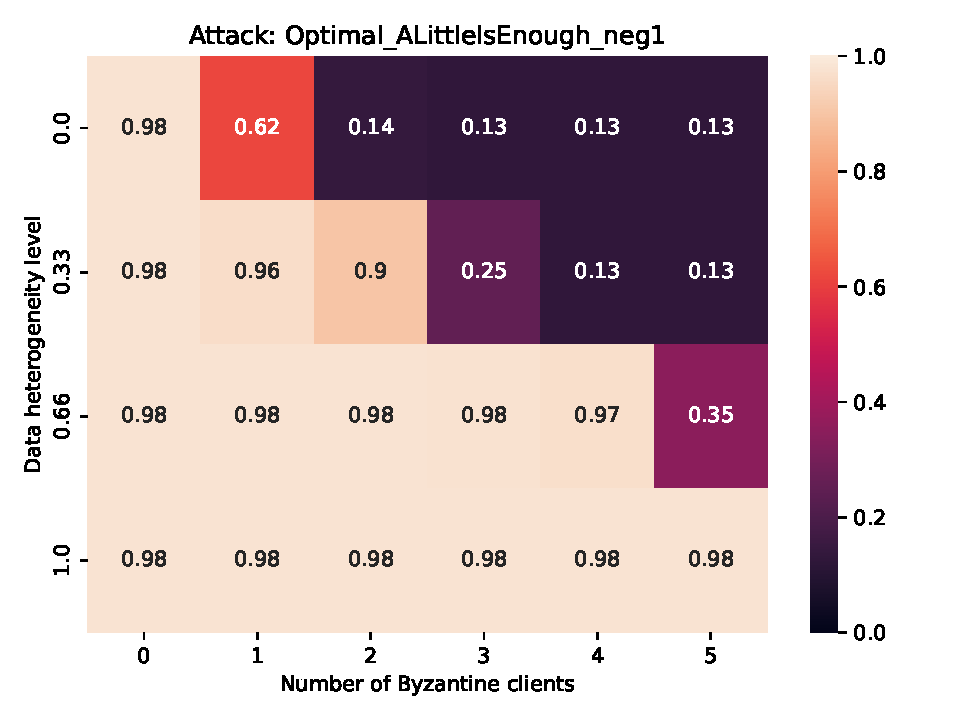
\includegraphics[width=\textwidth]{../plots/robust_new_atan_sweep/alpha_2.0/test_Optimal_ALittleIsEnough_neg1_mnist_cnn_mnist_snn_gamma_similarity_niid_NNM_ARC_MultiKrum_nb_honest_clients_10_tolerated_f_equal_real.pdf}
        \caption{$\alpha = 2.0$}
        \label{fig:mk_alie_alpha_2_0}
    \end{subfigure}
    \caption{Multi-Krum performance under Optimal ALIE across $\alpha$ values.}
    \label{fig:mk_alie_grid}
\end{figure}\clearpage
\subsubsection{MK under Sign Flipping Attack}
\begin{figure}[htbp]
    \centering
    \begin{subfigure}[b]{0.24\textwidth}
        \centering
        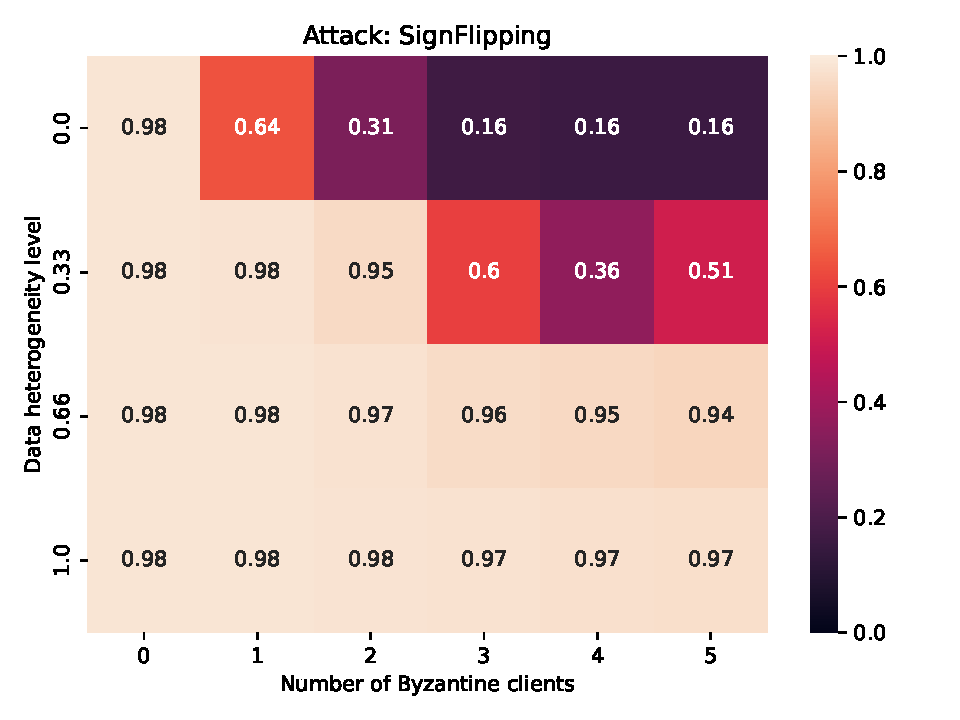
\includegraphics[width=\textwidth]{../plots/robust_comparison_sweep/test_SignFlipping_mnist_cnn_mnist_gamma_similarity_niid_NNM_ARC_MultiKrum_nb_honest_clients_10_tolerated_f_equal_real.pdf}
        \caption{CNN Baseline}
        \label{fig:mk_sf_cnn}
    \end{subfigure}
    \hfill
    \begin{subfigure}[b]{0.24\textwidth}
        \centering
        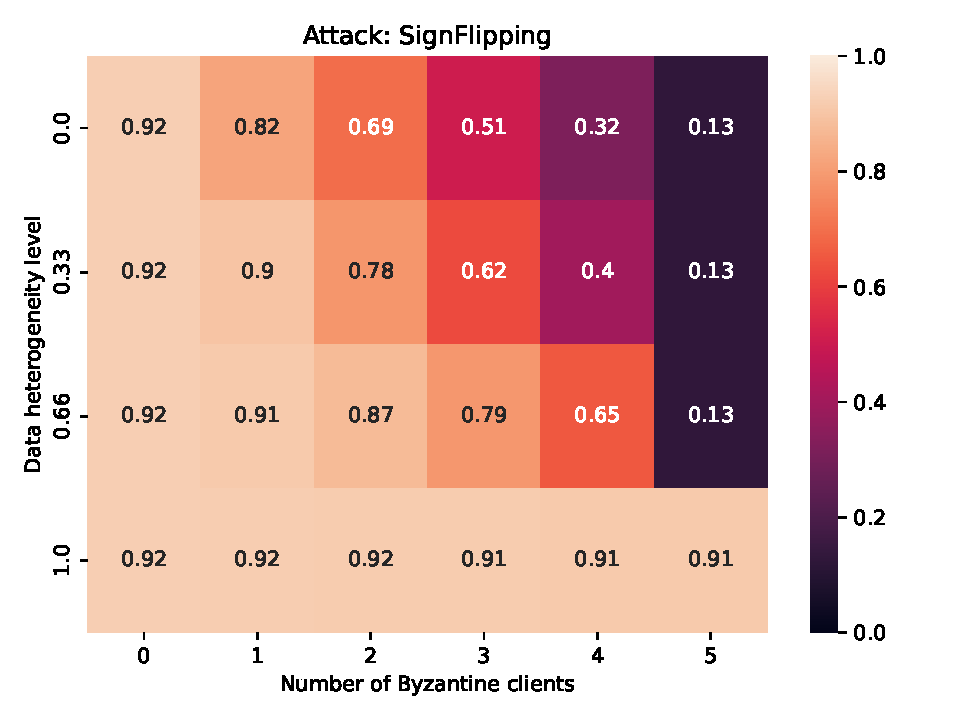
\includegraphics[width=\textwidth]{../plots/robust_new_atan_sweep/alpha_0.5/test_SignFlipping_mnist_cnn_mnist_snn_gamma_similarity_niid_NNM_ARC_MultiKrum_nb_honest_clients_10_tolerated_f_equal_real.pdf}
        \caption{$\alpha = 0.5$}
        \label{fig:mk_sf_alpha_0_5}
    \end{subfigure}
    \hfill
    \begin{subfigure}[b]{0.24\textwidth}
        \centering
        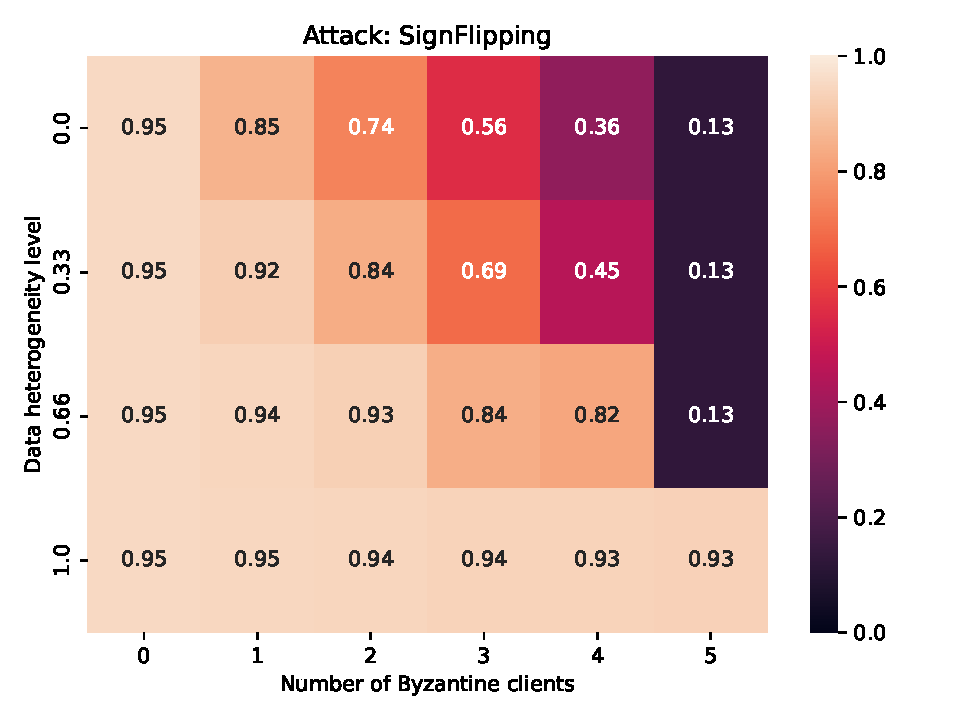
\includegraphics[width=\textwidth]{../plots/robust_new_atan_sweep/alpha_0.75/test_SignFlipping_mnist_cnn_mnist_snn_gamma_similarity_niid_NNM_ARC_MultiKrum_nb_honest_clients_10_tolerated_f_equal_real.pdf}
        \caption{$\alpha = 0.75$}
        \label{fig:mk_sf_alpha_0_75}
    \end{subfigure}
    \hfill
    \begin{subfigure}[b]{0.24\textwidth}
        \centering
        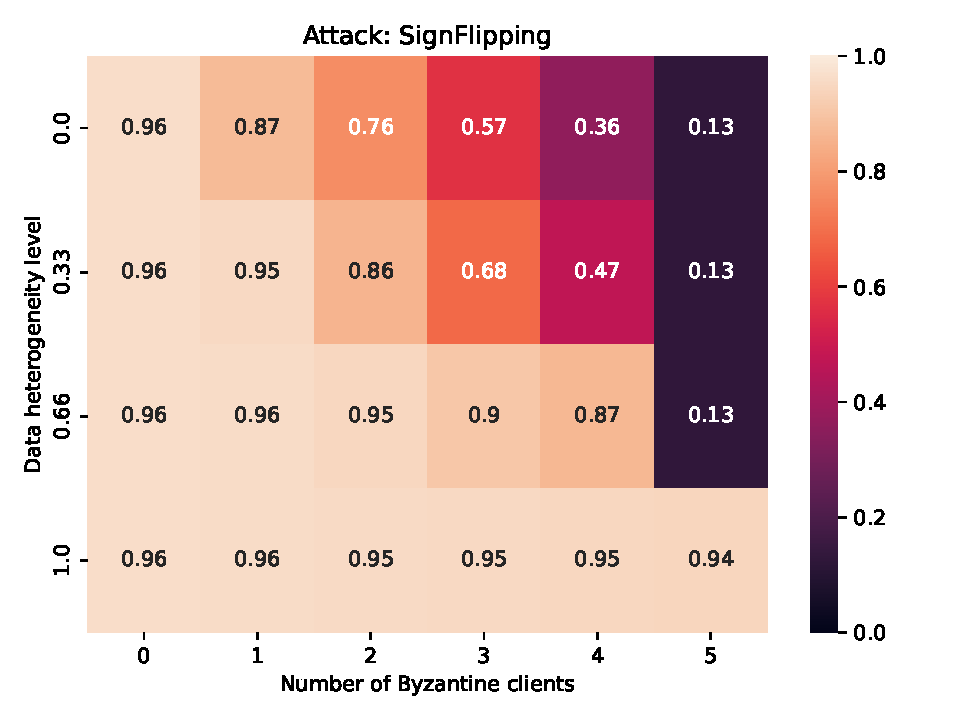
\includegraphics[width=\textwidth]{../plots/robust_new_atan_sweep/alpha_1.0/test_SignFlipping_mnist_cnn_mnist_snn_gamma_similarity_niid_NNM_ARC_MultiKrum_nb_honest_clients_10_tolerated_f_equal_real.pdf}
        \caption{$\alpha = 1.0$}
        \label{fig:mk_sf_alpha_1_0}
    \end{subfigure}
    \vspace{0.2cm}
    \begin{subfigure}[b]{0.24\textwidth}
        \centering
        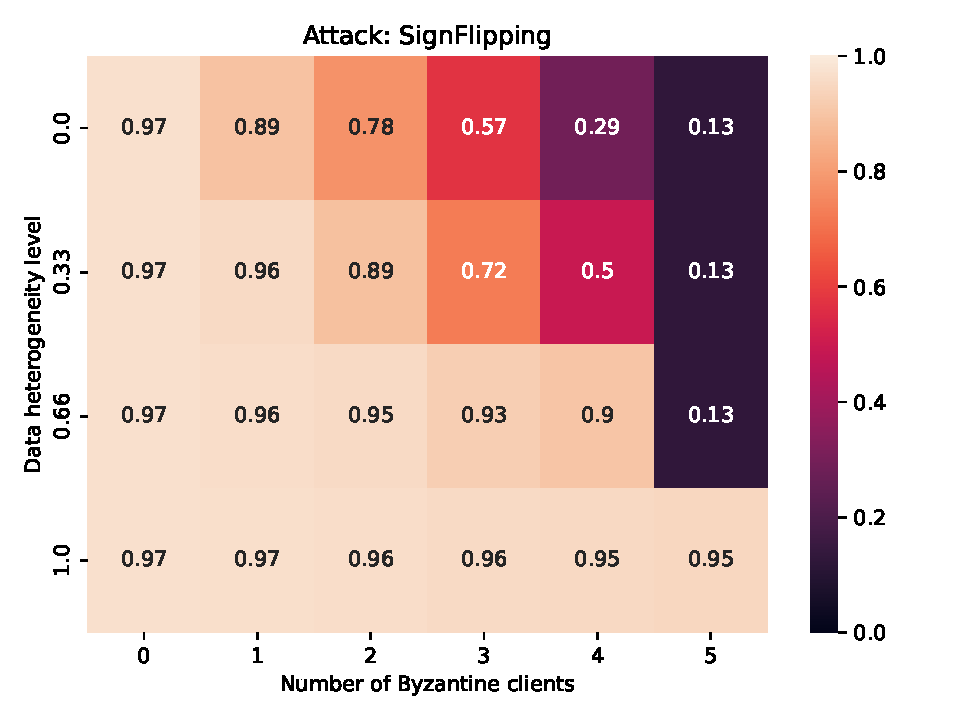
\includegraphics[width=\textwidth]{../plots/robust_new_atan_sweep/alpha_1.2/test_SignFlipping_mnist_cnn_mnist_snn_gamma_similarity_niid_NNM_ARC_MultiKrum_nb_honest_clients_10_tolerated_f_equal_real.pdf}
        \caption{$\alpha = 1.2$}
        \label{fig:mk_sf_alpha_1_2}
    \end{subfigure}
    \hfill
    \begin{subfigure}[b]{0.24\textwidth}
        \centering
        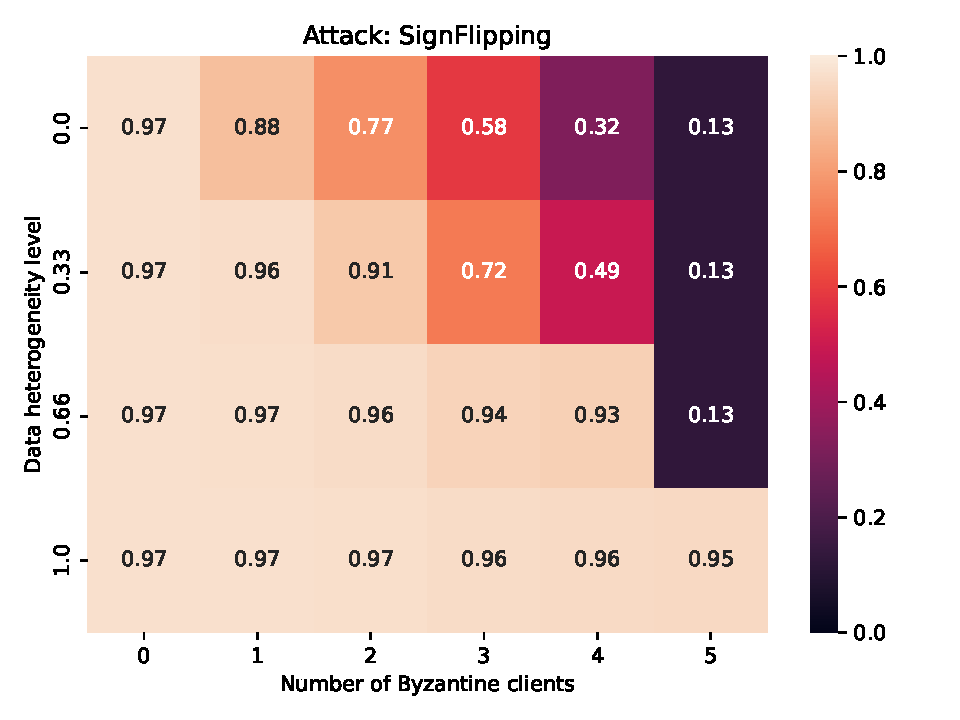
\includegraphics[width=\textwidth]{../plots/robust_new_atan_sweep/alpha_1.4/test_SignFlipping_mnist_cnn_mnist_snn_gamma_similarity_niid_NNM_ARC_MultiKrum_nb_honest_clients_10_tolerated_f_equal_real.pdf}
        \caption{$\alpha = 1.4$}
        \label{fig:mk_sf_alpha_1_4}
    \end{subfigure}
    \hfill
    \begin{subfigure}[b]{0.24\textwidth}
        \centering
        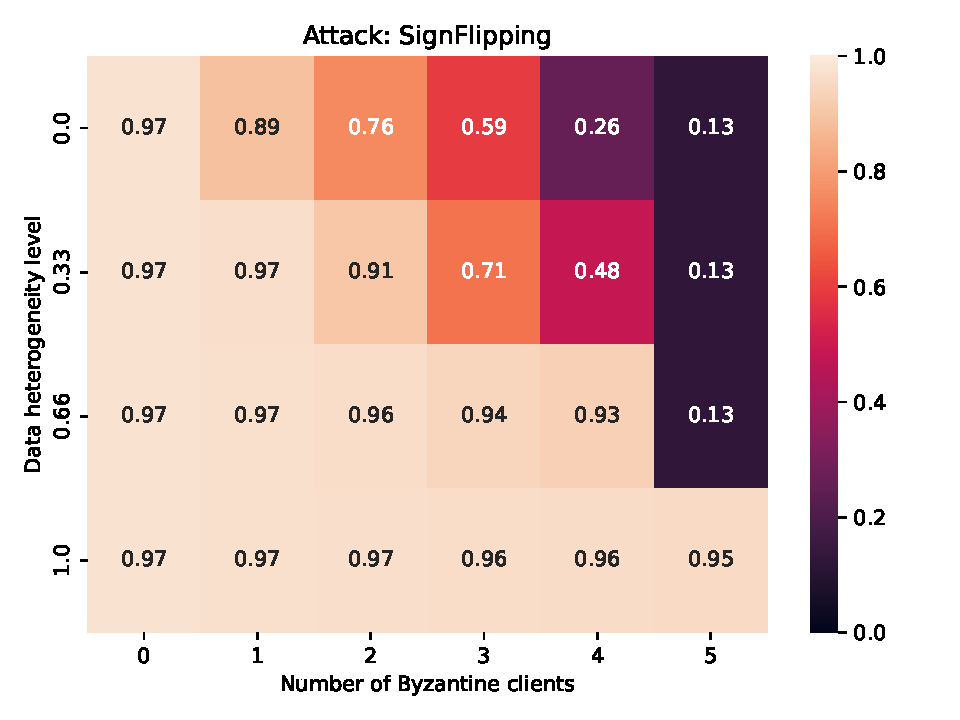
\includegraphics[width=\textwidth]{../plots/robust_new_atan_sweep/alpha_1.5/test_SignFlipping_mnist_cnn_mnist_snn_gamma_similarity_niid_NNM_ARC_MultiKrum_nb_honest_clients_10_tolerated_f_equal_real.pdf}
        \caption{$\alpha = 1.5$}
        \label{fig:mk_sf_alpha_1_5}
    \end{subfigure}
    \hfill
    \begin{subfigure}[b]{0.24\textwidth}
        \centering
        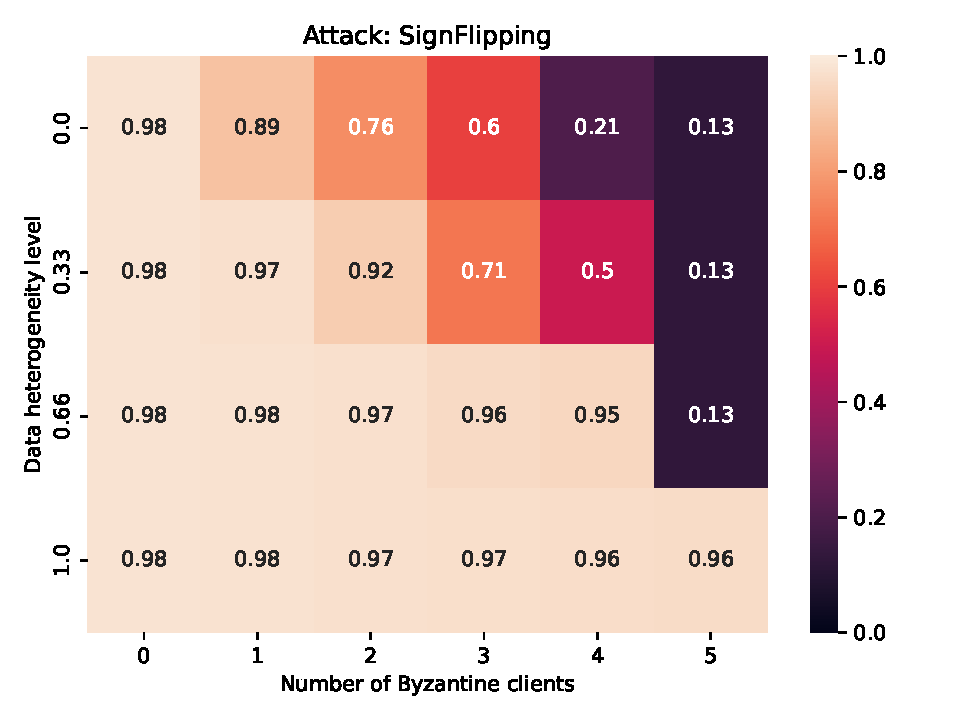
\includegraphics[width=\textwidth]{../plots/robust_new_atan_sweep/alpha_2.0/test_SignFlipping_mnist_cnn_mnist_snn_gamma_similarity_niid_NNM_ARC_MultiKrum_nb_honest_clients_10_tolerated_f_equal_real.pdf}
        \caption{$\alpha = 2.0$}
        \label{fig:mk_sf_alpha_2_0}
    \end{subfigure}
    \caption{Multi-Krum performance under Sign Flipping across $\alpha$ values.}
    \label{fig:mk_sf_grid}
\end{figure}\clearpage
\subsubsection{MK under Optimal Inner Product Manipulation Attack}
\begin{figure}[htbp]
    \centering
    \begin{subfigure}[b]{0.24\textwidth}
        \centering
        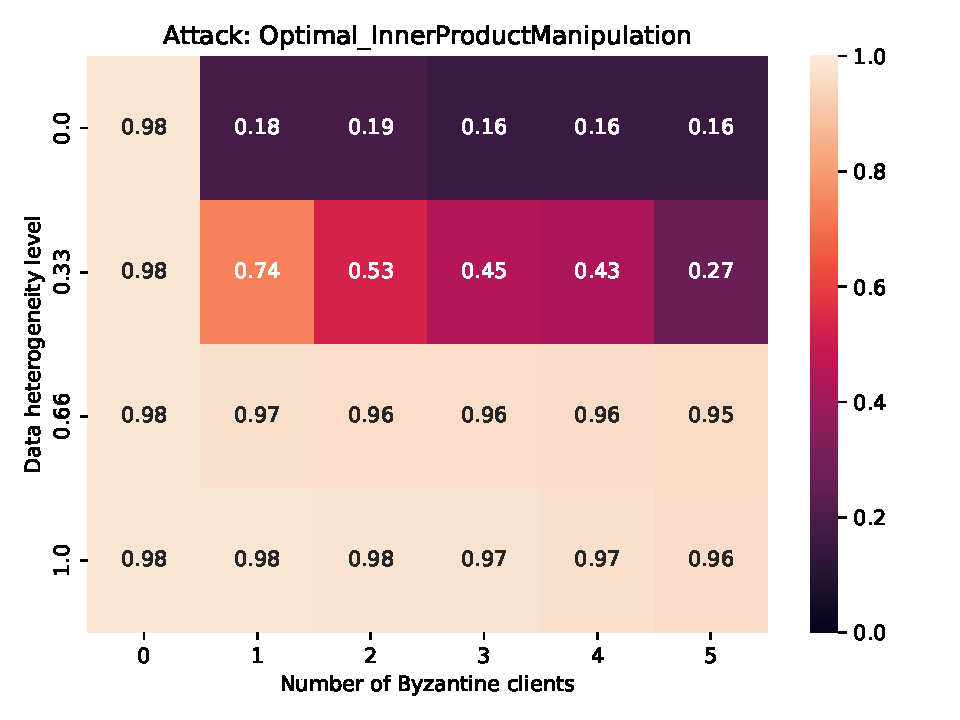
\includegraphics[width=\textwidth]{../plots/robust_comparison_sweep/test_Optimal_InnerProductManipulation_mnist_cnn_mnist_gamma_similarity_niid_NNM_ARC_MultiKrum_nb_honest_clients_10_tolerated_f_equal_real.pdf}
        \caption{CNN Baseline}
        \label{fig:mk_ipm_cnn}
    \end{subfigure}
    \hfill
    \begin{subfigure}[b]{0.24\textwidth}
        \centering
        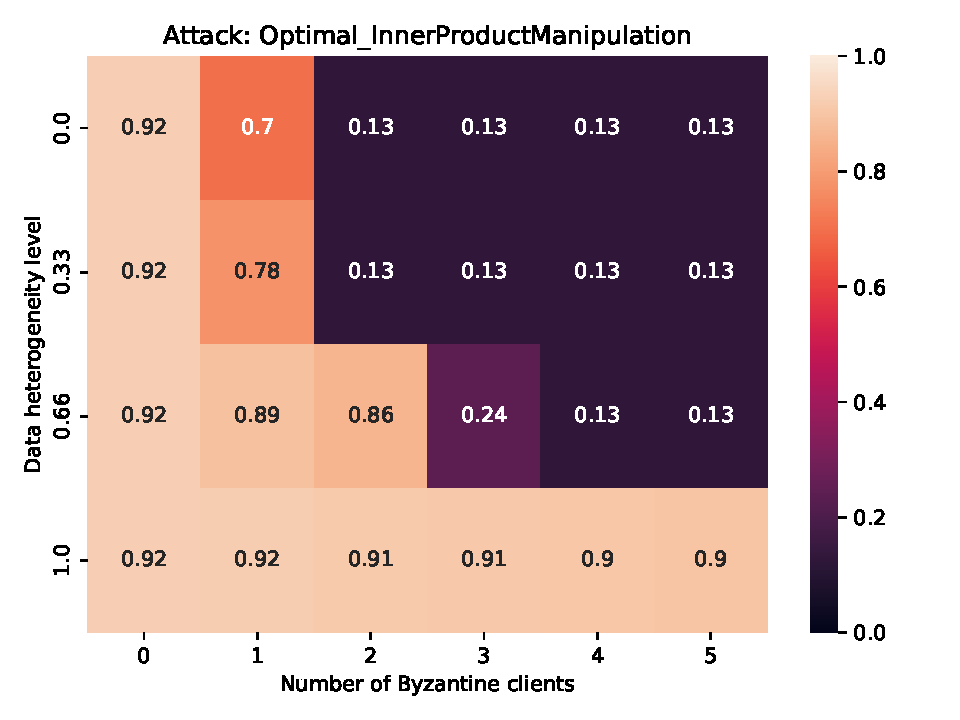
\includegraphics[width=\textwidth]{../plots/robust_new_atan_sweep/alpha_0.5/test_Optimal_InnerProductManipulation_mnist_cnn_mnist_snn_gamma_similarity_niid_NNM_ARC_MultiKrum_nb_honest_clients_10_tolerated_f_equal_real.pdf}
        \caption{$\alpha = 0.5$}
        \label{fig:mk_ipm_alpha_0_5}
    \end{subfigure}
    \hfill
    \begin{subfigure}[b]{0.24\textwidth}
        \centering
        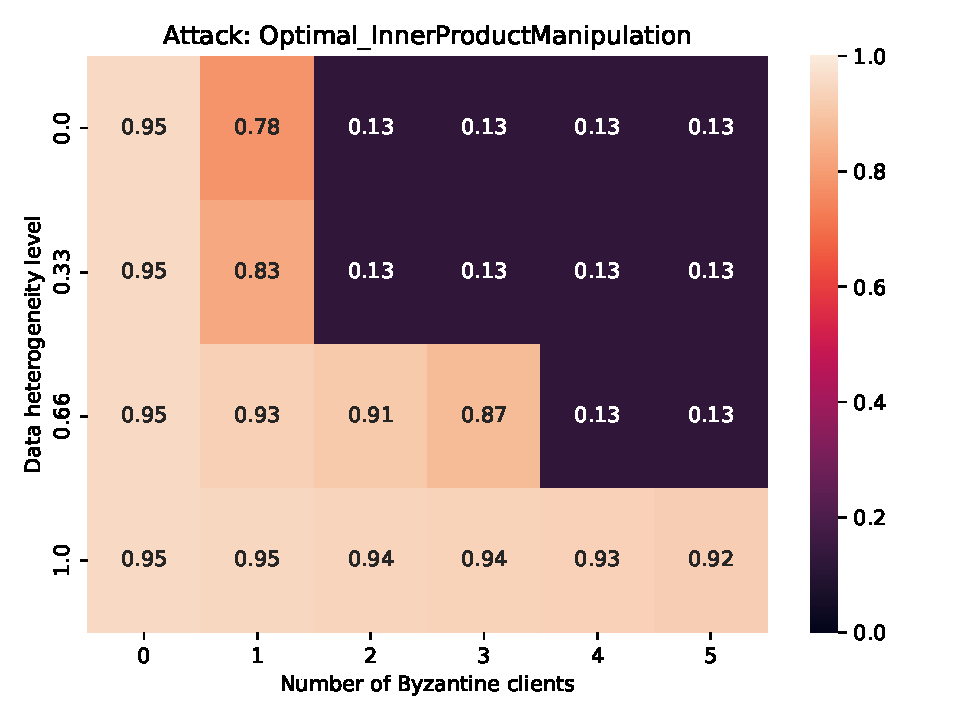
\includegraphics[width=\textwidth]{../plots/robust_new_atan_sweep/alpha_0.75/test_Optimal_InnerProductManipulation_mnist_cnn_mnist_snn_gamma_similarity_niid_NNM_ARC_MultiKrum_nb_honest_clients_10_tolerated_f_equal_real.pdf}
        \caption{$\alpha = 0.75$}
        \label{fig:mk_ipm_alpha_0_75}
    \end{subfigure}
    \hfill
    \begin{subfigure}[b]{0.24\textwidth}
        \centering
        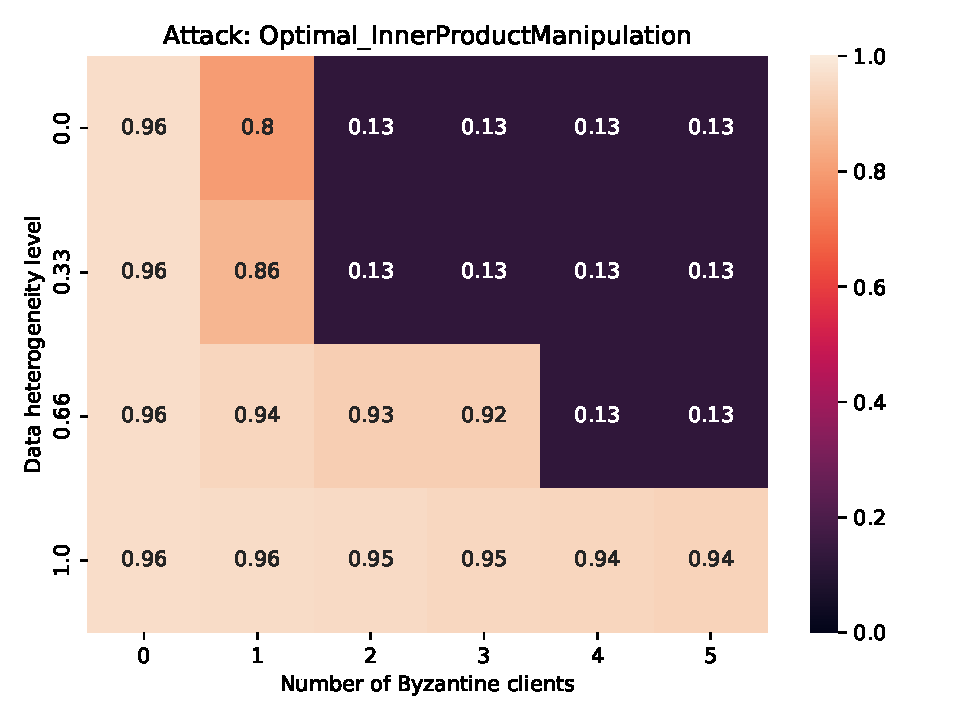
\includegraphics[width=\textwidth]{../plots/robust_new_atan_sweep/alpha_1.0/test_Optimal_InnerProductManipulation_mnist_cnn_mnist_snn_gamma_similarity_niid_NNM_ARC_MultiKrum_nb_honest_clients_10_tolerated_f_equal_real.pdf}
        \caption{$\alpha = 1.0$}
        \label{fig:mk_ipm_alpha_1_0}
    \end{subfigure}
    \vspace{0.2cm}
    \begin{subfigure}[b]{0.24\textwidth}
        \centering
        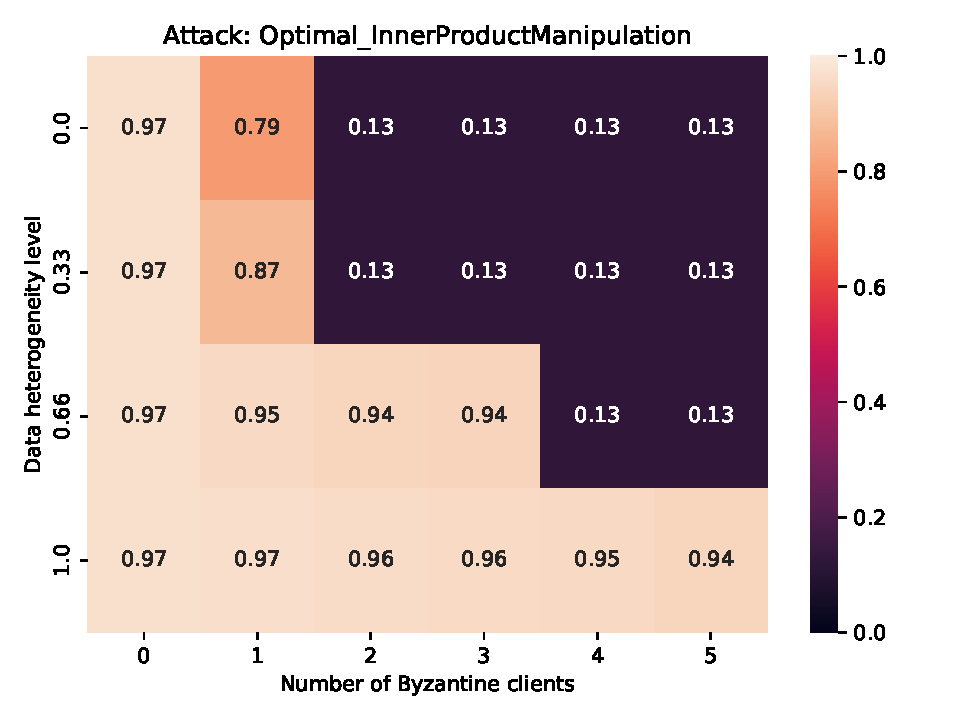
\includegraphics[width=\textwidth]{../plots/robust_new_atan_sweep/alpha_1.2/test_Optimal_InnerProductManipulation_mnist_cnn_mnist_snn_gamma_similarity_niid_NNM_ARC_MultiKrum_nb_honest_clients_10_tolerated_f_equal_real.pdf}
        \caption{$\alpha = 1.2$}
        \label{fig:mk_ipm_alpha_1_2}
    \end{subfigure}
    \hfill
    \begin{subfigure}[b]{0.24\textwidth}
        \centering
        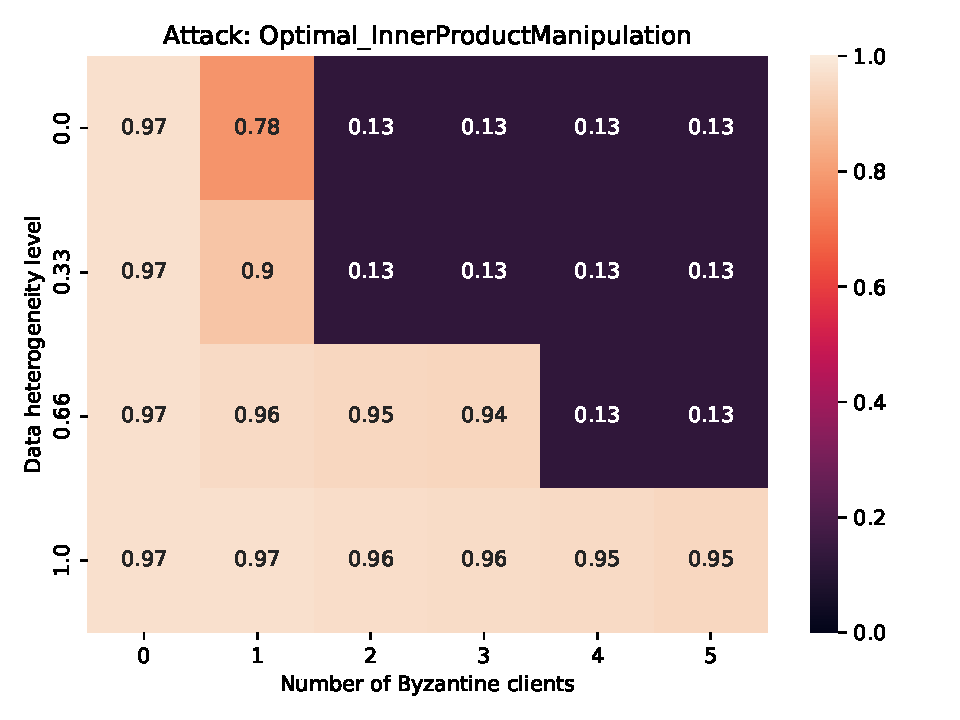
\includegraphics[width=\textwidth]{../plots/robust_new_atan_sweep/alpha_1.4/test_Optimal_InnerProductManipulation_mnist_cnn_mnist_snn_gamma_similarity_niid_NNM_ARC_MultiKrum_nb_honest_clients_10_tolerated_f_equal_real.pdf}
        \caption{$\alpha = 1.4$}
        \label{fig:mk_ipm_alpha_1_4}
    \end{subfigure}
    \hfill
    \begin{subfigure}[b]{0.24\textwidth}
        \centering
        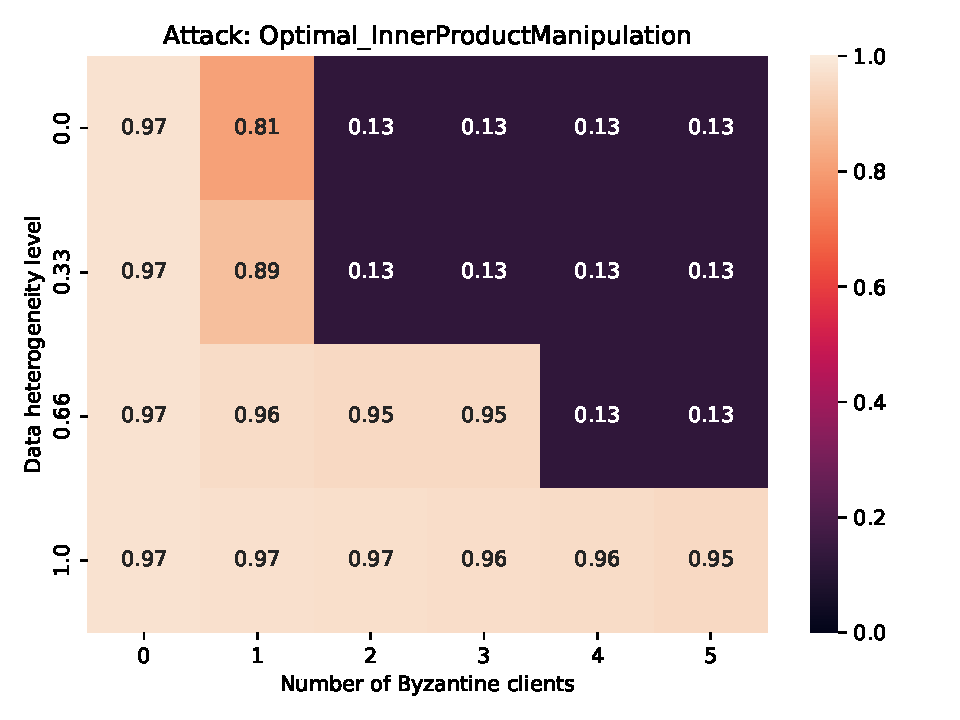
\includegraphics[width=\textwidth]{../plots/robust_new_atan_sweep/alpha_1.5/test_Optimal_InnerProductManipulation_mnist_cnn_mnist_snn_gamma_similarity_niid_NNM_ARC_MultiKrum_nb_honest_clients_10_tolerated_f_equal_real.pdf}
        \caption{$\alpha = 1.5$}
        \label{fig:mk_ipm_alpha_1_5}
    \end{subfigure}
    \hfill
    \begin{subfigure}[b]{0.24\textwidth}
        \centering
        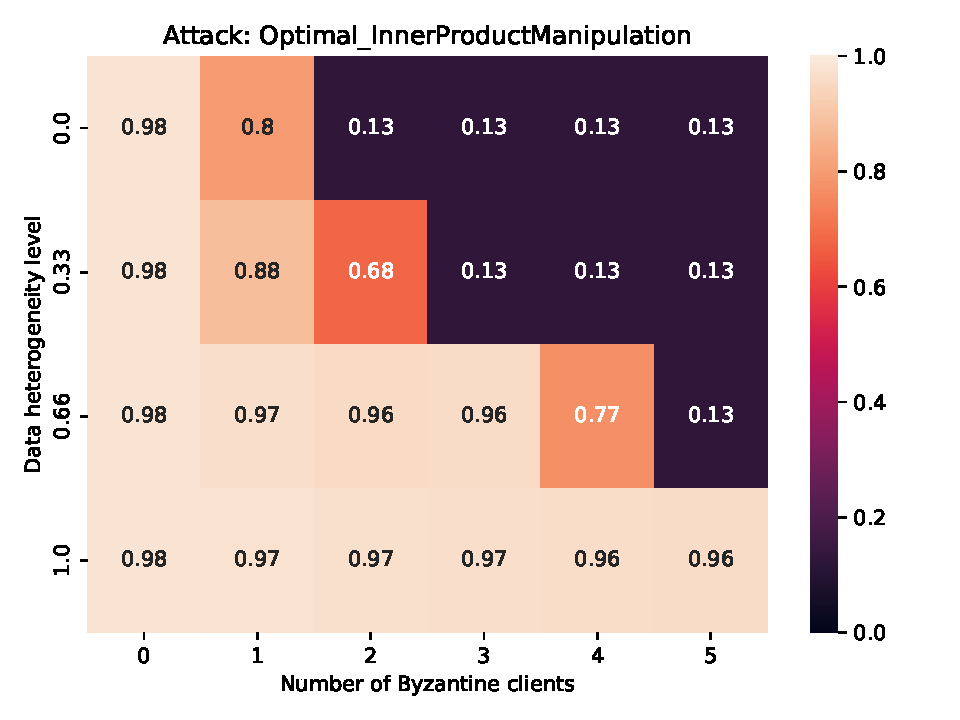
\includegraphics[width=\textwidth]{../plots/robust_new_atan_sweep/alpha_2.0/test_Optimal_InnerProductManipulation_mnist_cnn_mnist_snn_gamma_similarity_niid_NNM_ARC_MultiKrum_nb_honest_clients_10_tolerated_f_equal_real.pdf}
        \caption{$\alpha = 2.0$}
        \label{fig:mk_ipm_alpha_2_0}
    \end{subfigure}
    \caption{Multi-Krum performance under Optimal Inner Product Manipulation across $\alpha$ values.}
    \label{fig:mk_ipm_grid}
\end{figure}
\clearpage
\subsection{Trimmed Mean (TM)}
\subsubsection{TM under Worst-Case across all Attacks}
\begin{figure}[htbp]
    \centering
    \begin{subfigure}[b]{0.24\textwidth}
        \centering
        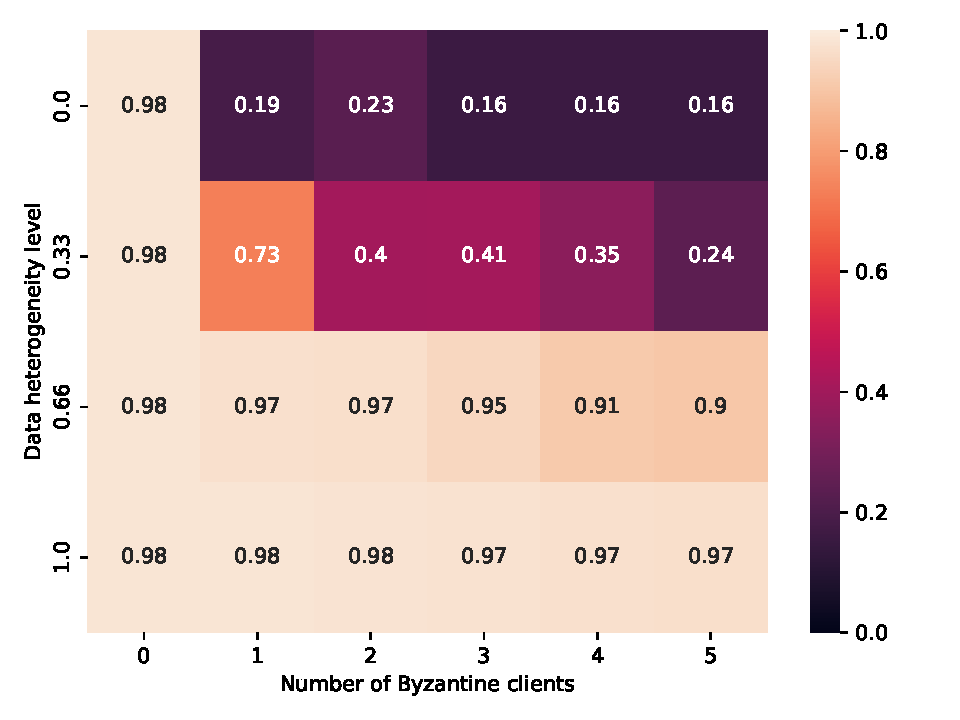
\includegraphics[width=\textwidth]{../plots/robust_comparison_sweep/test_mnist_cnn_mnist_gamma_similarity_niid_NNM_ARC_TrMean_nb_honest_clients_10_tolerated_f_equal_real.pdf}
        \caption{CNN Baseline}
        \label{fig:tm_worst_case_cnn}
    \end{subfigure}
    \hfill
    \begin{subfigure}[b]{0.24\textwidth}
        \centering
        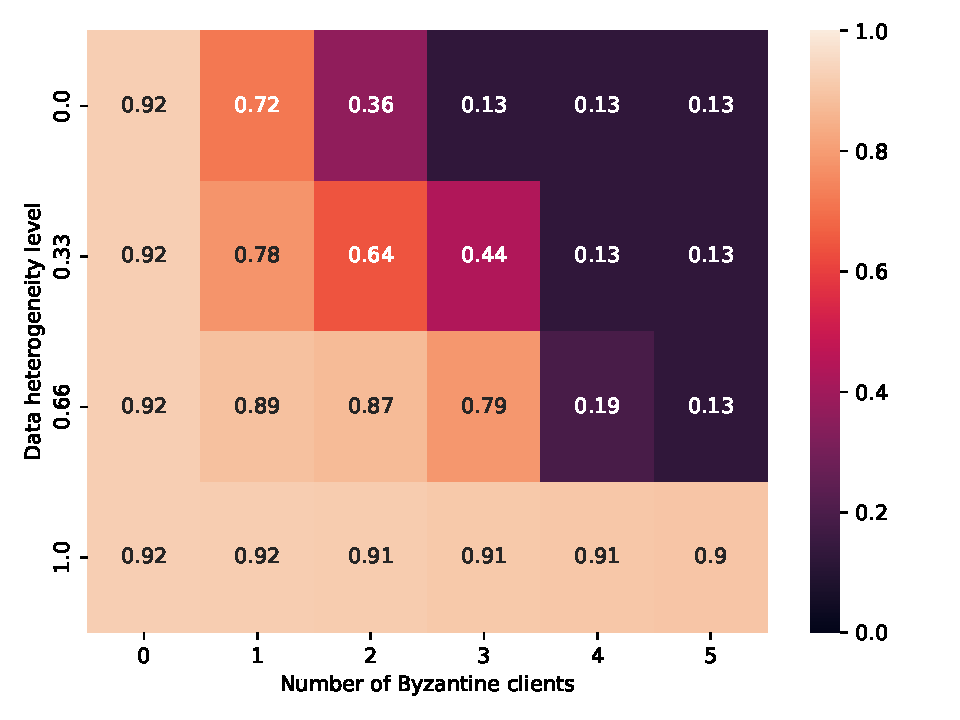
\includegraphics[width=\textwidth]{../plots/robust_new_atan_sweep/alpha_0.5/test_mnist_cnn_mnist_snn_gamma_similarity_niid_NNM_ARC_TrMean_nb_honest_clients_10_tolerated_f_equal_real.pdf}
        \caption{$\alpha = 0.5$}
        \label{fig:tm_worst_case_alpha_0_5}
    \end{subfigure}
    \hfill
    \begin{subfigure}[b]{0.24\textwidth}
        \centering
        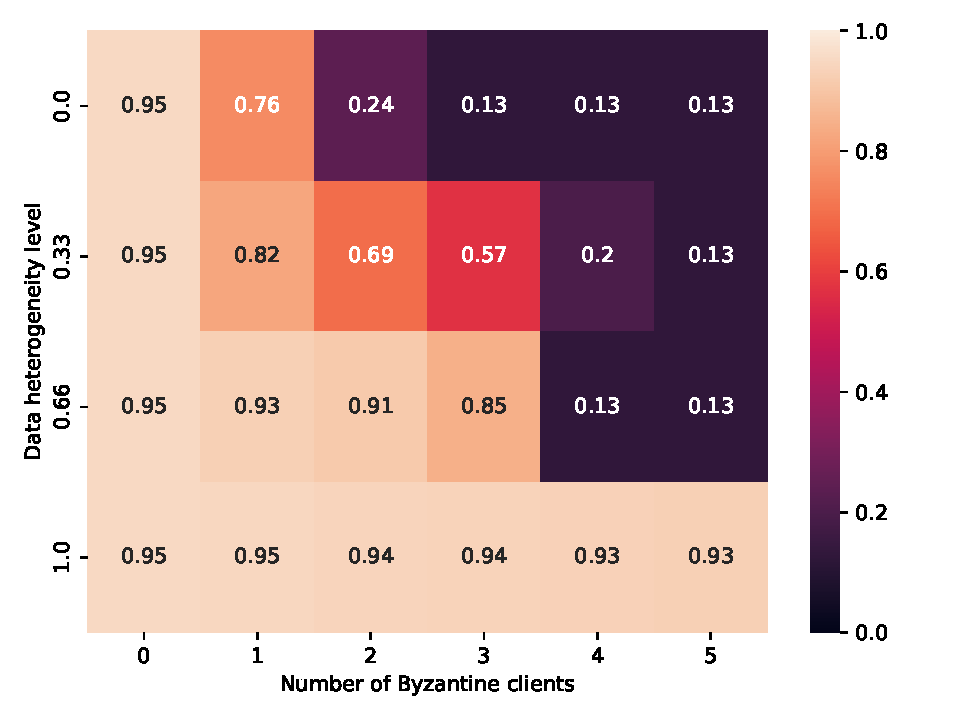
\includegraphics[width=\textwidth]{../plots/robust_new_atan_sweep/alpha_0.75/test_mnist_cnn_mnist_snn_gamma_similarity_niid_NNM_ARC_TrMean_nb_honest_clients_10_tolerated_f_equal_real.pdf}
        \caption{$\alpha = 0.75$}
        \label{fig:tm_worst_case_alpha_0_75}
    \end{subfigure}
    \hfill
    \begin{subfigure}[b]{0.24\textwidth}
        \centering
        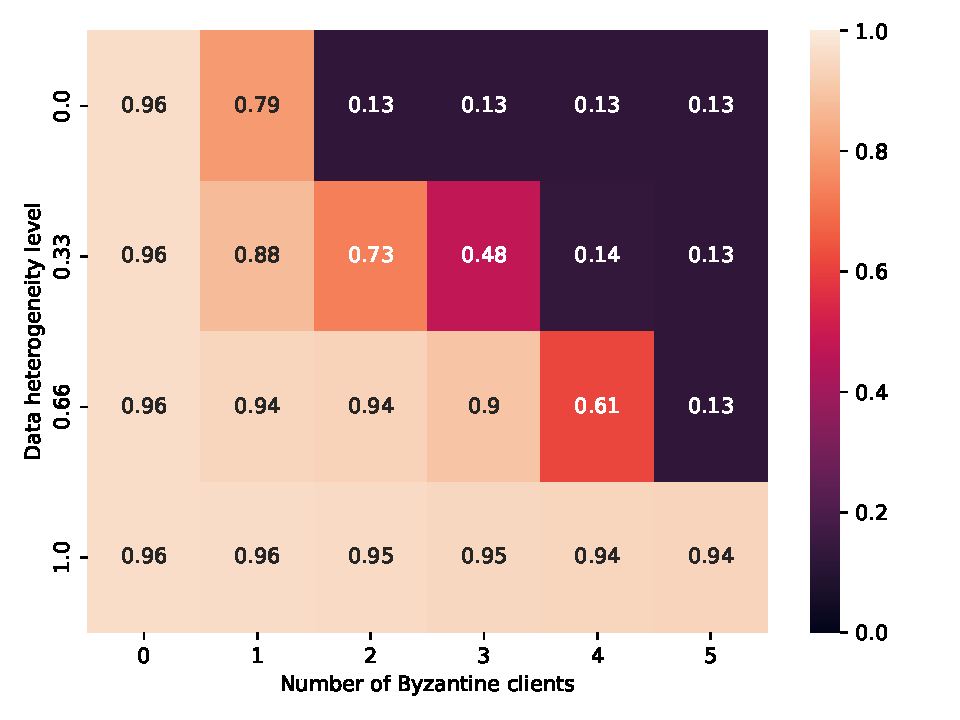
\includegraphics[width=\textwidth]{../plots/robust_new_atan_sweep/alpha_1.0/test_mnist_cnn_mnist_snn_gamma_similarity_niid_NNM_ARC_TrMean_nb_honest_clients_10_tolerated_f_equal_real.pdf}
        \caption{$\alpha = 1.0$}
        \label{fig:tm_worst_case_alpha_1_0}
    \end{subfigure}
    \vspace{0.2cm}
    \begin{subfigure}[b]{0.24\textwidth}
        \centering
        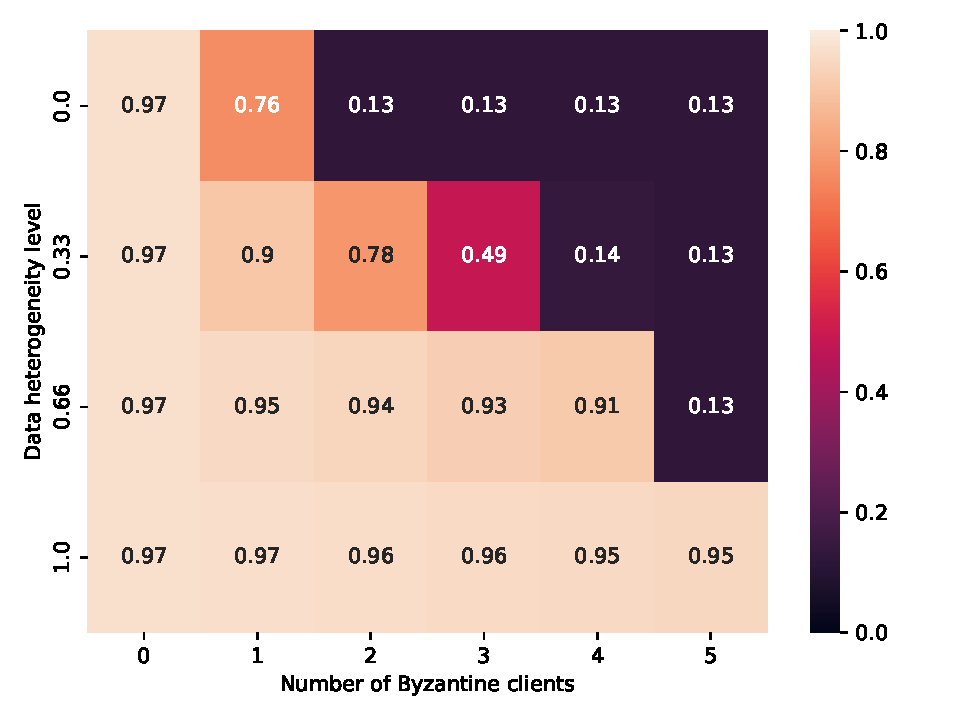
\includegraphics[width=\textwidth]{../plots/robust_new_atan_sweep/alpha_1.2/test_mnist_cnn_mnist_snn_gamma_similarity_niid_NNM_ARC_TrMean_nb_honest_clients_10_tolerated_f_equal_real.pdf}
        \caption{$\alpha = 1.2$}
        \label{fig:tm_worst_case_alpha_1_2}
    \end{subfigure}
    \hfill
    \begin{subfigure}[b]{0.24\textwidth}
        \centering
        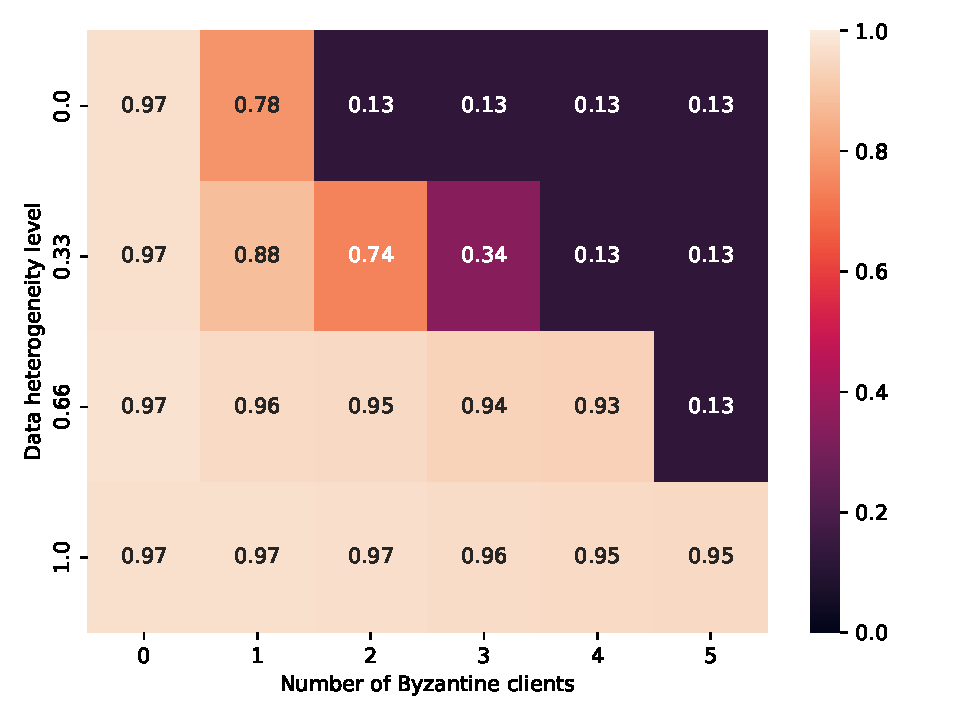
\includegraphics[width=\textwidth]{../plots/robust_new_atan_sweep/alpha_1.4/test_mnist_cnn_mnist_snn_gamma_similarity_niid_NNM_ARC_TrMean_nb_honest_clients_10_tolerated_f_equal_real.pdf}
        \caption{$\alpha = 1.4$}
        \label{fig:tm_worst_case_alpha_1_4}
    \end{subfigure}
    \hfill
    \begin{subfigure}[b]{0.24\textwidth}
        \centering
        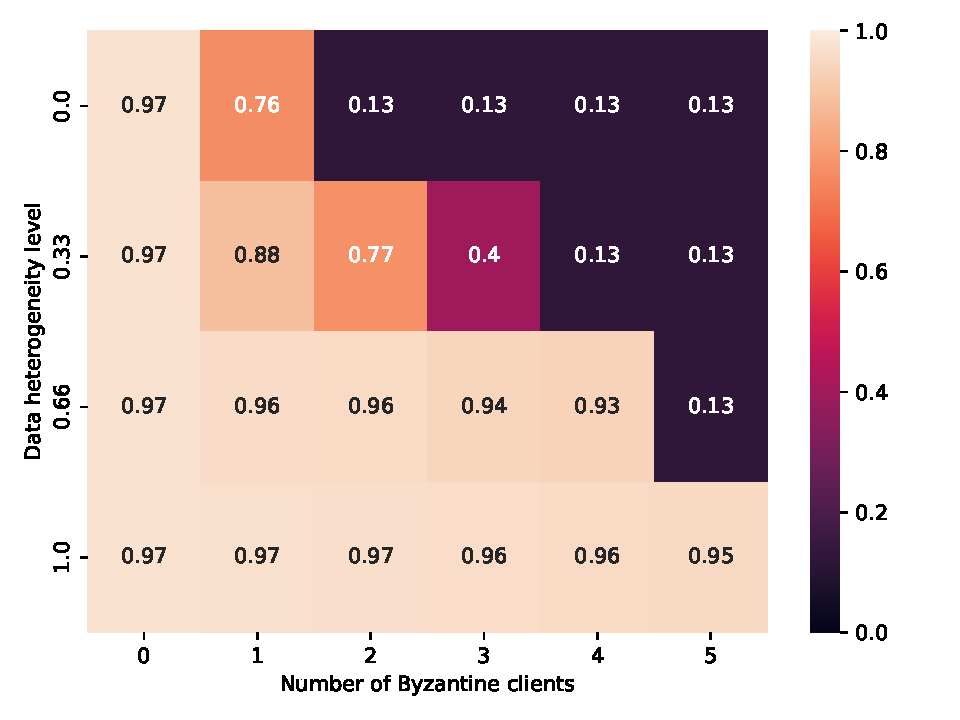
\includegraphics[width=\textwidth]{../plots/robust_new_atan_sweep/alpha_1.5/test_mnist_cnn_mnist_snn_gamma_similarity_niid_NNM_ARC_TrMean_nb_honest_clients_10_tolerated_f_equal_real.pdf}
        \caption{$\alpha = 1.5$}
        \label{fig:tm_worst_case_alpha_1_5}
    \end{subfigure}
    \hfill
    \begin{subfigure}[b]{0.24\textwidth}
        \centering
        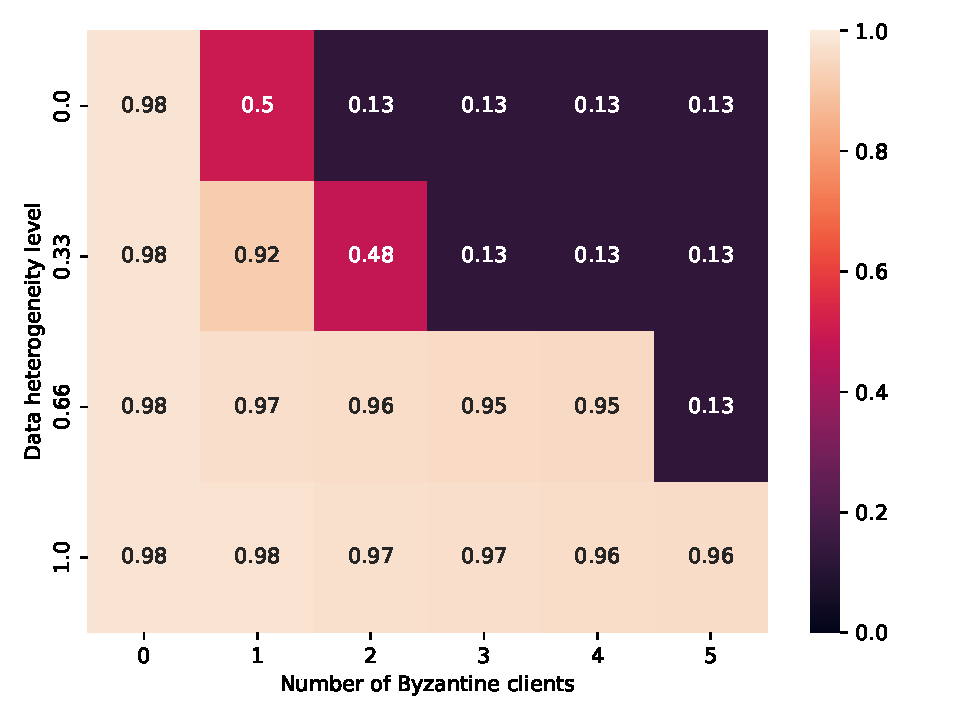
\includegraphics[width=\textwidth]{../plots/robust_new_atan_sweep/alpha_2.0/test_mnist_cnn_mnist_snn_gamma_similarity_niid_NNM_ARC_TrMean_nb_honest_clients_10_tolerated_f_equal_real.pdf}
        \caption{$\alpha = 2.0$}
        \label{fig:tm_worst_case_alpha_2_0}
    \end{subfigure}
    \caption{Trimmed Mean performance under the worst-case across all attacks across $\alpha$ values.}
    \label{fig:tm_worst_case_grid}
\end{figure}\clearpage
\subsubsection{TM under Optimal ALIE Attack}
\begin{figure}[htbp]
    \centering
    \begin{subfigure}[b]{0.24\textwidth}
        \centering
        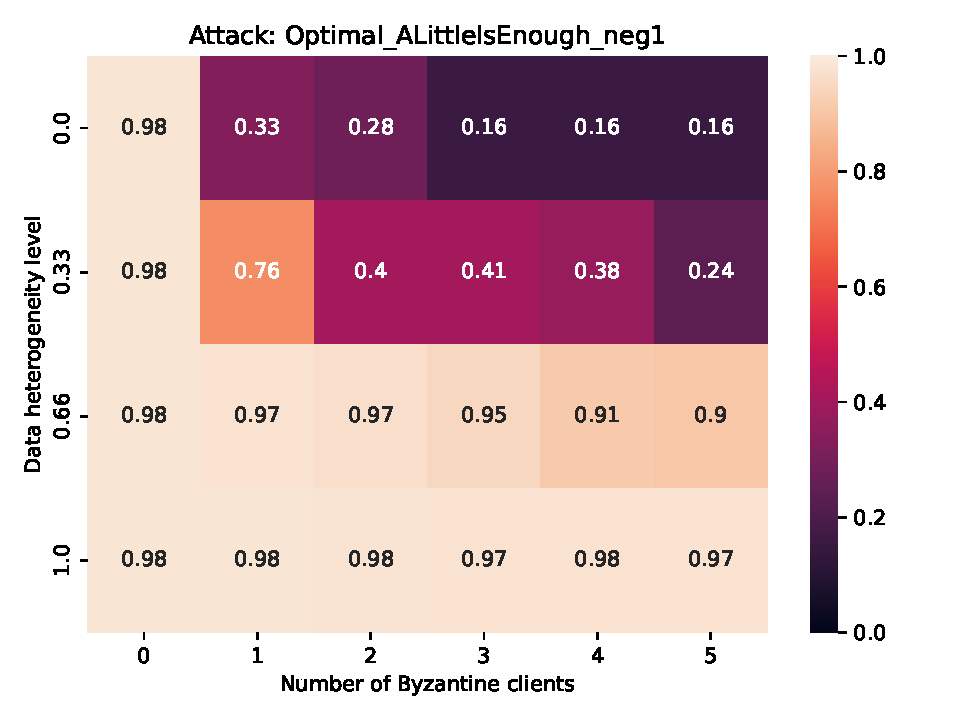
\includegraphics[width=\textwidth]{../plots/robust_comparison_sweep/test_Optimal_ALittleIsEnough_neg1_mnist_cnn_mnist_gamma_similarity_niid_NNM_ARC_TrMean_nb_honest_clients_10_tolerated_f_equal_real.pdf}
        \caption{CNN Baseline}
        \label{fig:tm_alie_cnn}
    \end{subfigure}
    \hfill
    \begin{subfigure}[b]{0.24\textwidth}
        \centering
        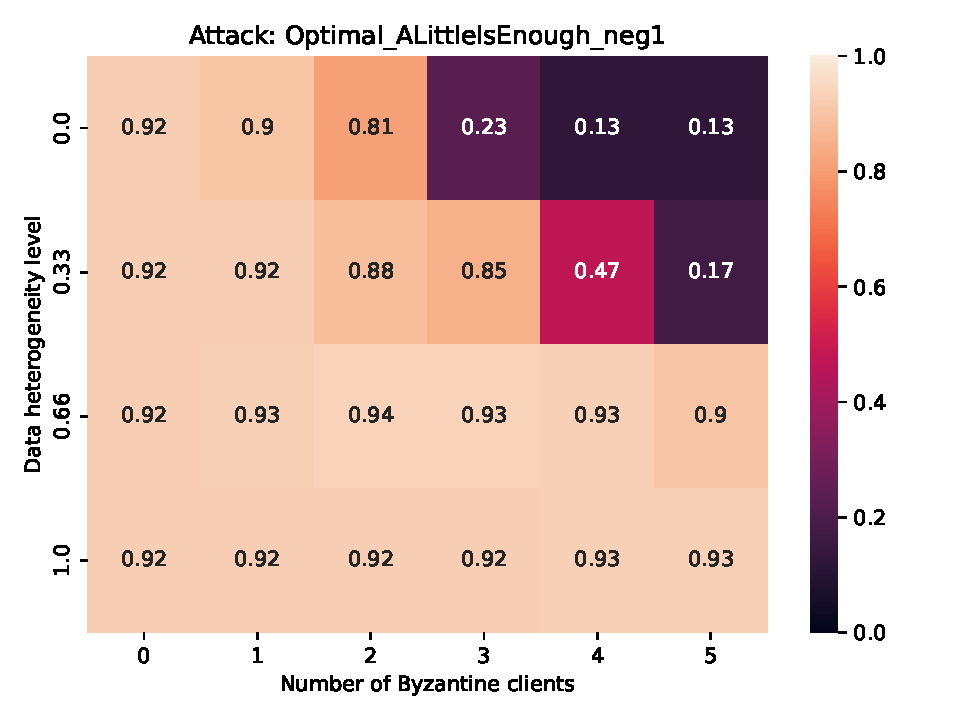
\includegraphics[width=\textwidth]{../plots/robust_new_atan_sweep/alpha_0.5/test_Optimal_ALittleIsEnough_neg1_mnist_cnn_mnist_snn_gamma_similarity_niid_NNM_ARC_TrMean_nb_honest_clients_10_tolerated_f_equal_real.pdf}
        \caption{$\alpha = 0.5$}
        \label{fig:tm_alie_alpha_0_5}
    \end{subfigure}
    \hfill
    \begin{subfigure}[b]{0.24\textwidth}
        \centering
        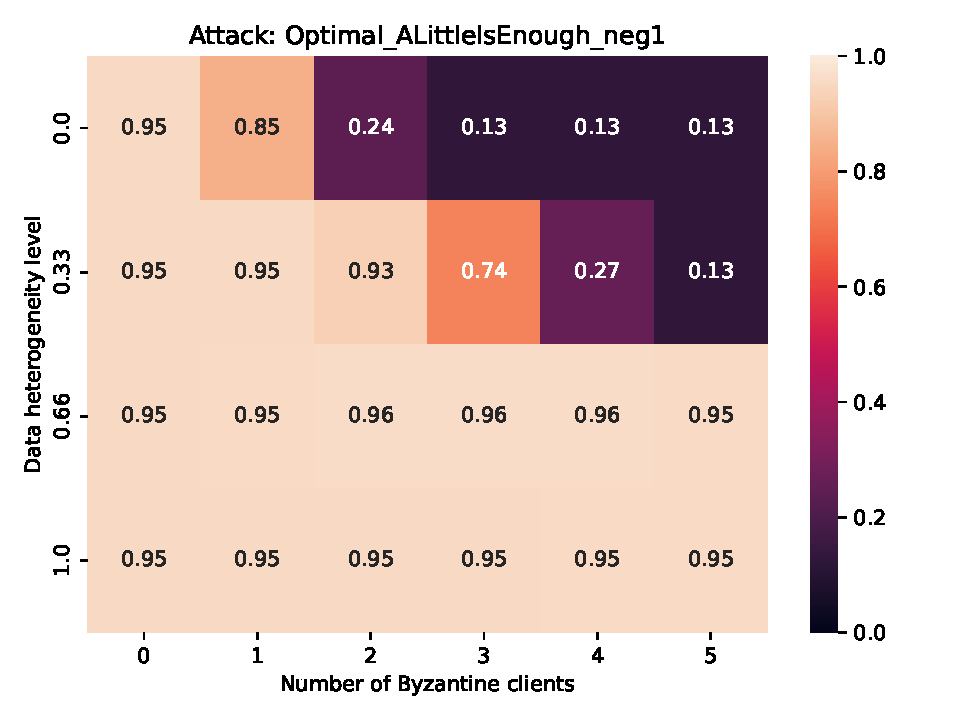
\includegraphics[width=\textwidth]{../plots/robust_new_atan_sweep/alpha_0.75/test_Optimal_ALittleIsEnough_neg1_mnist_cnn_mnist_snn_gamma_similarity_niid_NNM_ARC_TrMean_nb_honest_clients_10_tolerated_f_equal_real.pdf}
        \caption{$\alpha = 0.75$}
        \label{fig:tm_alie_alpha_0_75}
    \end{subfigure}
    \hfill
    \begin{subfigure}[b]{0.24\textwidth}
        \centering
        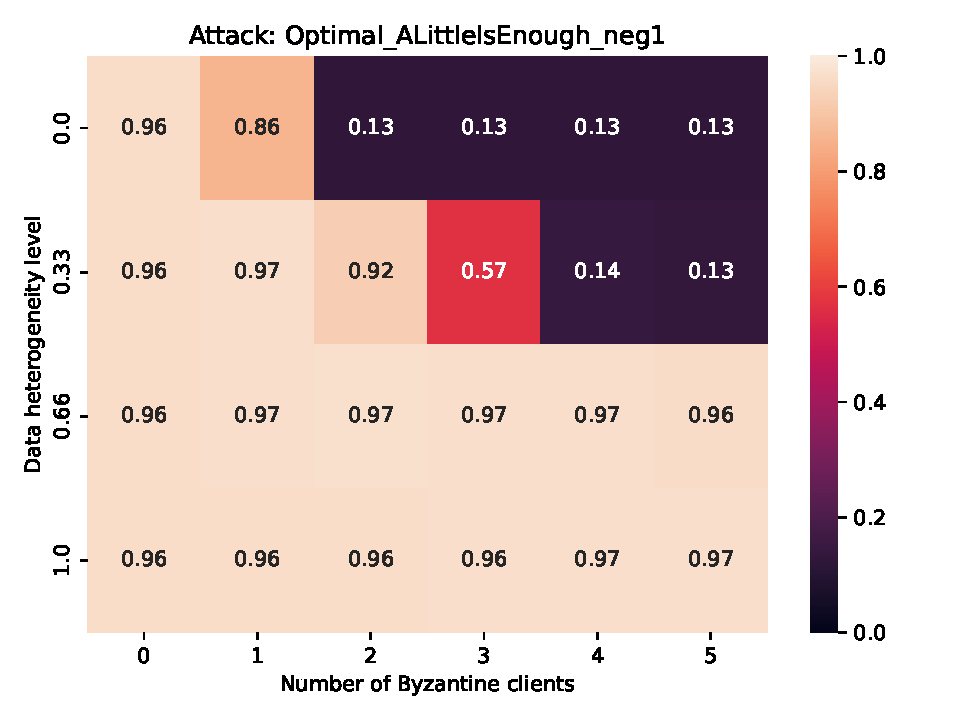
\includegraphics[width=\textwidth]{../plots/robust_new_atan_sweep/alpha_1.0/test_Optimal_ALittleIsEnough_neg1_mnist_cnn_mnist_snn_gamma_similarity_niid_NNM_ARC_TrMean_nb_honest_clients_10_tolerated_f_equal_real.pdf}
        \caption{$\alpha = 1.0$}
        \label{fig:tm_alie_alpha_1_0}
    \end{subfigure}
    \vspace{0.2cm}
    \begin{subfigure}[b]{0.24\textwidth}
        \centering
        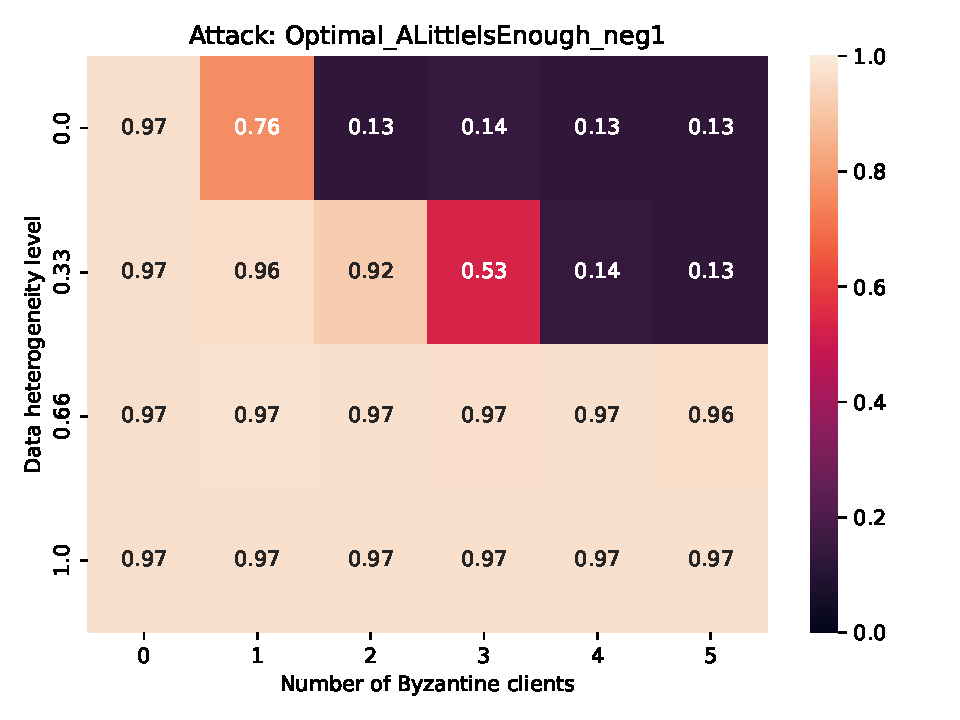
\includegraphics[width=\textwidth]{../plots/robust_new_atan_sweep/alpha_1.2/test_Optimal_ALittleIsEnough_neg1_mnist_cnn_mnist_snn_gamma_similarity_niid_NNM_ARC_TrMean_nb_honest_clients_10_tolerated_f_equal_real.pdf}
        \caption{$\alpha = 1.2$}
        \label{fig:tm_alie_alpha_1_2}
    \end{subfigure}
    \hfill
    \begin{subfigure}[b]{0.24\textwidth}
        \centering
        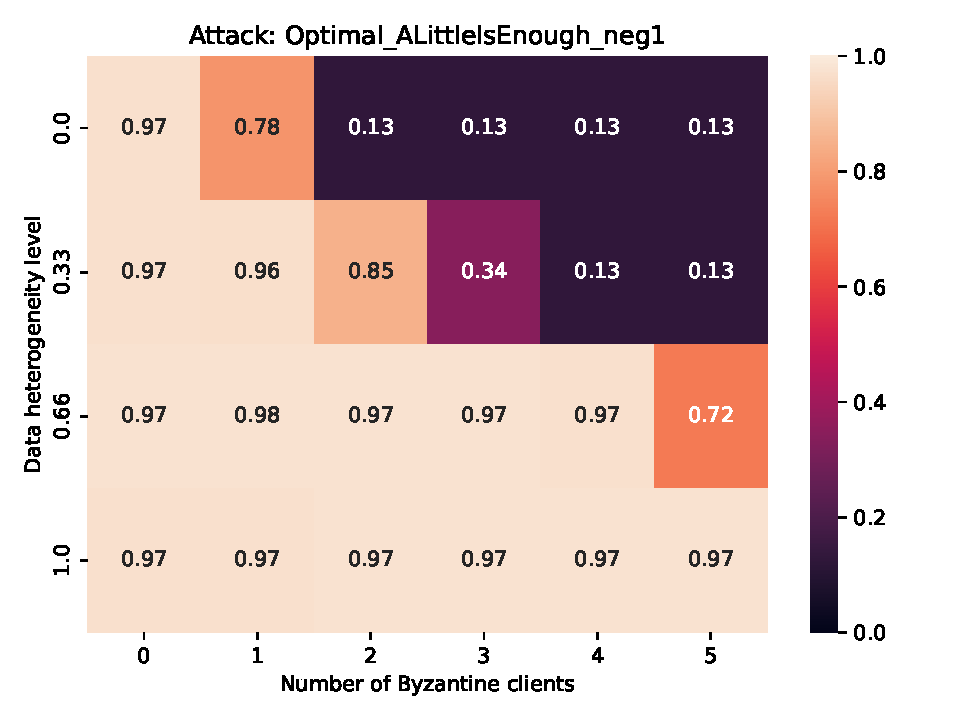
\includegraphics[width=\textwidth]{../plots/robust_new_atan_sweep/alpha_1.4/test_Optimal_ALittleIsEnough_neg1_mnist_cnn_mnist_snn_gamma_similarity_niid_NNM_ARC_TrMean_nb_honest_clients_10_tolerated_f_equal_real.pdf}
        \caption{$\alpha = 1.4$}
        \label{fig:tm_alie_alpha_1_4}
    \end{subfigure}
    \hfill
    \begin{subfigure}[b]{0.24\textwidth}
        \centering
        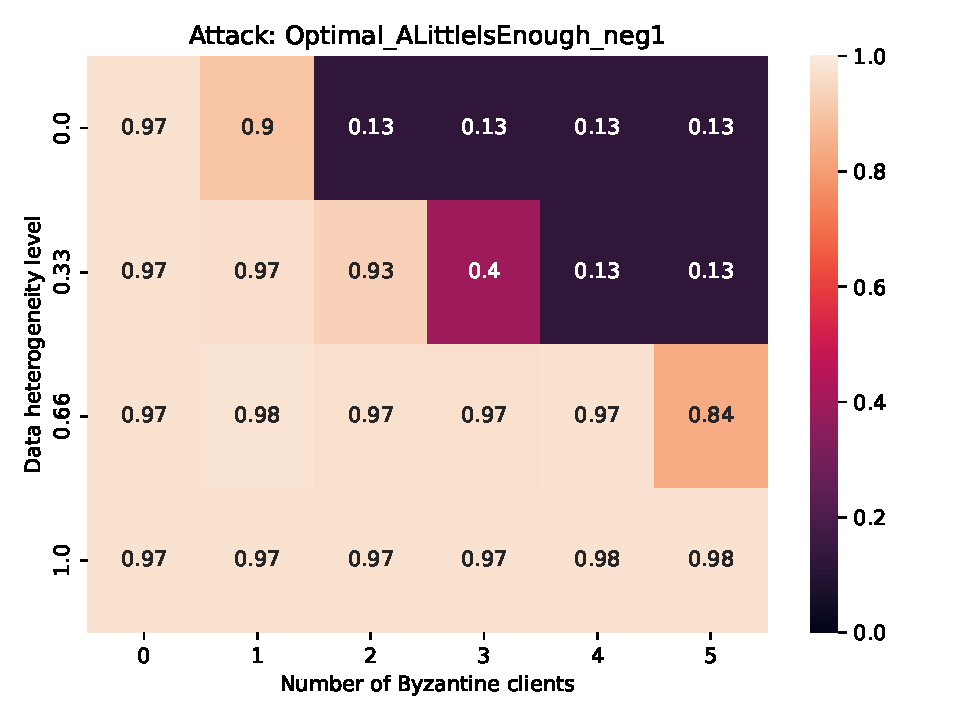
\includegraphics[width=\textwidth]{../plots/robust_new_atan_sweep/alpha_1.5/test_Optimal_ALittleIsEnough_neg1_mnist_cnn_mnist_snn_gamma_similarity_niid_NNM_ARC_TrMean_nb_honest_clients_10_tolerated_f_equal_real.pdf}
        \caption{$\alpha = 1.5$}
        \label{fig:tm_alie_alpha_1_5}
    \end{subfigure}
    \hfill
    \begin{subfigure}[b]{0.24\textwidth}
        \centering
        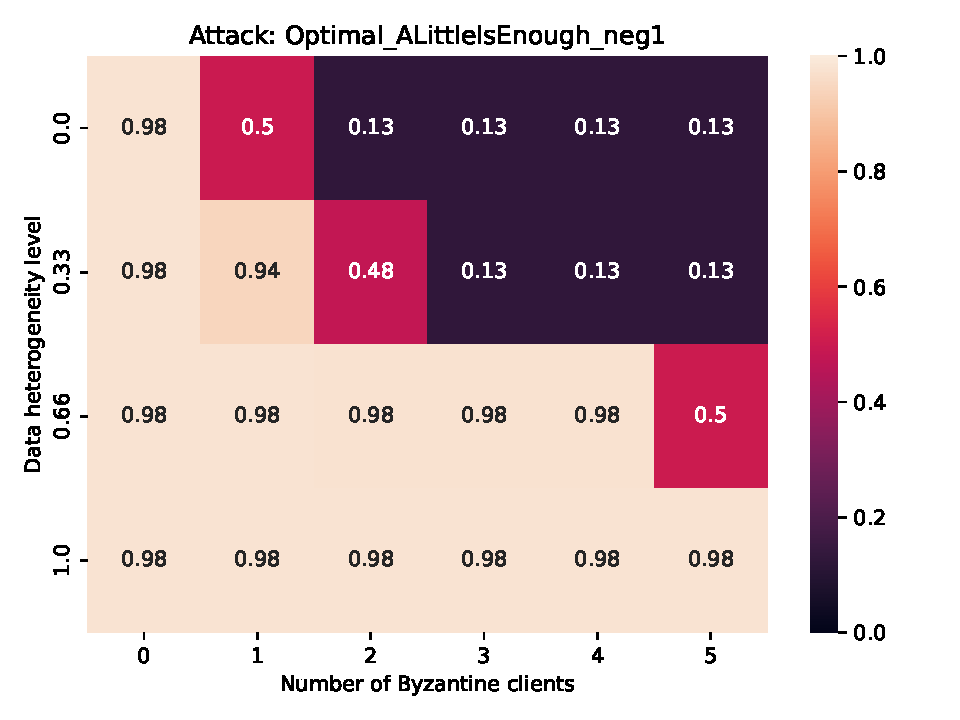
\includegraphics[width=\textwidth]{../plots/robust_new_atan_sweep/alpha_2.0/test_Optimal_ALittleIsEnough_neg1_mnist_cnn_mnist_snn_gamma_similarity_niid_NNM_ARC_TrMean_nb_honest_clients_10_tolerated_f_equal_real.pdf}
        \caption{$\alpha = 2.0$}
        \label{fig:tm_alie_alpha_2_0}
    \end{subfigure}
    \caption{Trimmed Mean performance under Optimal ALIE across $\alpha$ values.}
    \label{fig:tm_alie_grid}
\end{figure}\clearpage
\subsubsection{TM under Sign Flipping Attack}
\begin{figure}[htbp]
    \centering
    \begin{subfigure}[b]{0.24\textwidth}
        \centering
        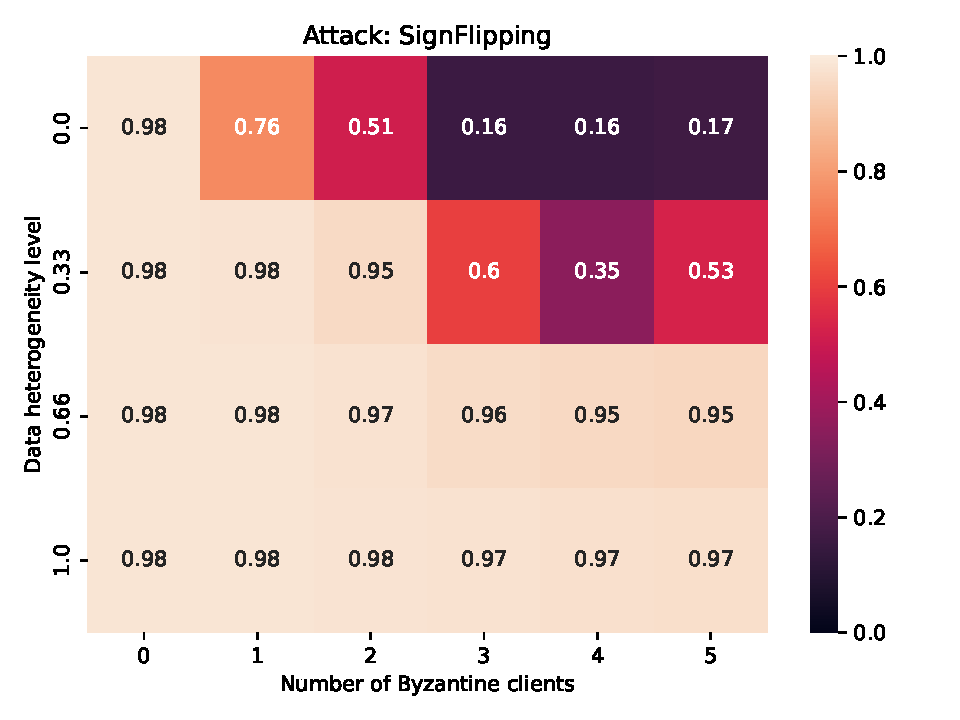
\includegraphics[width=\textwidth]{../plots/robust_comparison_sweep/test_SignFlipping_mnist_cnn_mnist_gamma_similarity_niid_NNM_ARC_TrMean_nb_honest_clients_10_tolerated_f_equal_real.pdf}
        \caption{CNN Baseline}
        \label{fig:tm_sf_cnn}
    \end{subfigure}
    \hfill
    \begin{subfigure}[b]{0.24\textwidth}
        \centering
        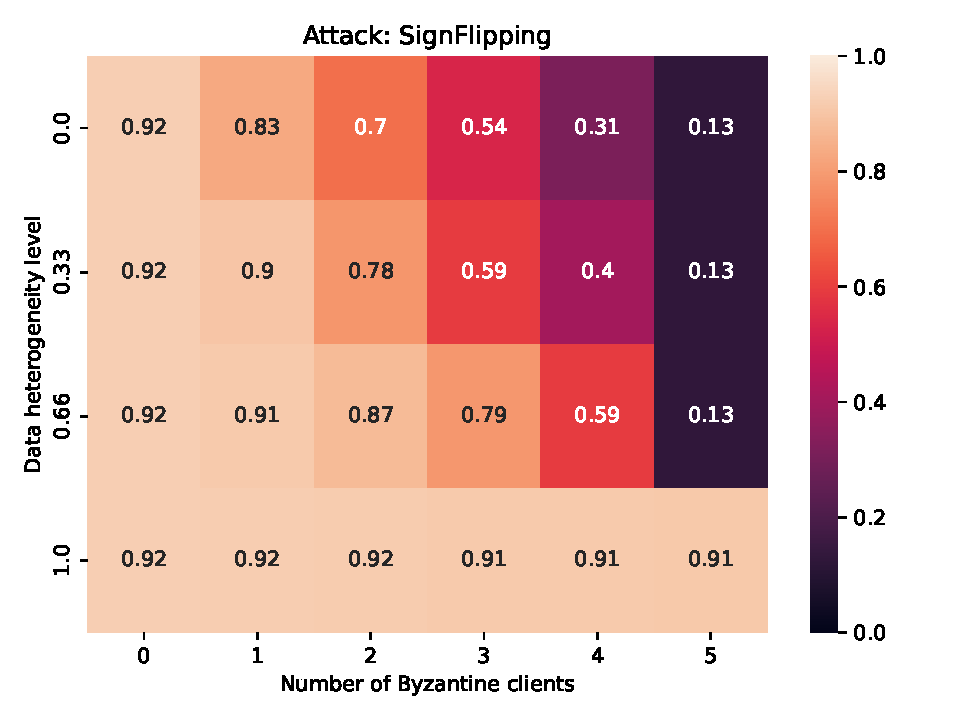
\includegraphics[width=\textwidth]{../plots/robust_new_atan_sweep/alpha_0.5/test_SignFlipping_mnist_cnn_mnist_snn_gamma_similarity_niid_NNM_ARC_TrMean_nb_honest_clients_10_tolerated_f_equal_real.pdf}
        \caption{$\alpha = 0.5$}
        \label{fig:tm_sf_alpha_0_5}
    \end{subfigure}
    \hfill
    \begin{subfigure}[b]{0.24\textwidth}
        \centering
        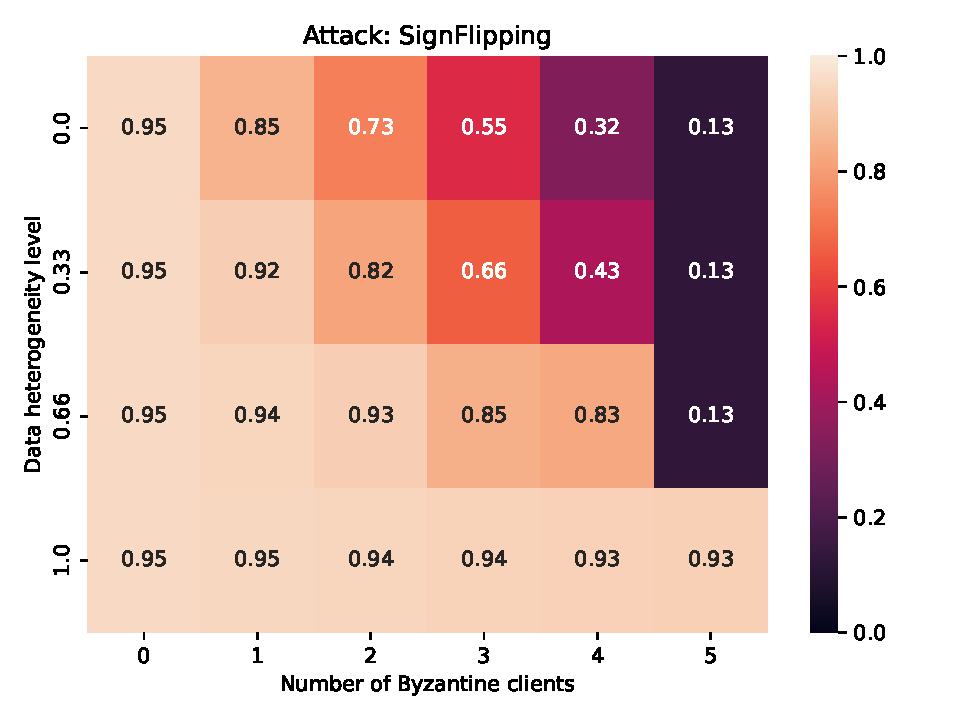
\includegraphics[width=\textwidth]{../plots/robust_new_atan_sweep/alpha_0.75/test_SignFlipping_mnist_cnn_mnist_snn_gamma_similarity_niid_NNM_ARC_TrMean_nb_honest_clients_10_tolerated_f_equal_real.pdf}
        \caption{$\alpha = 0.75$}
        \label{fig:tm_sf_alpha_0_75}
    \end{subfigure}
    \hfill
    \begin{subfigure}[b]{0.24\textwidth}
        \centering
        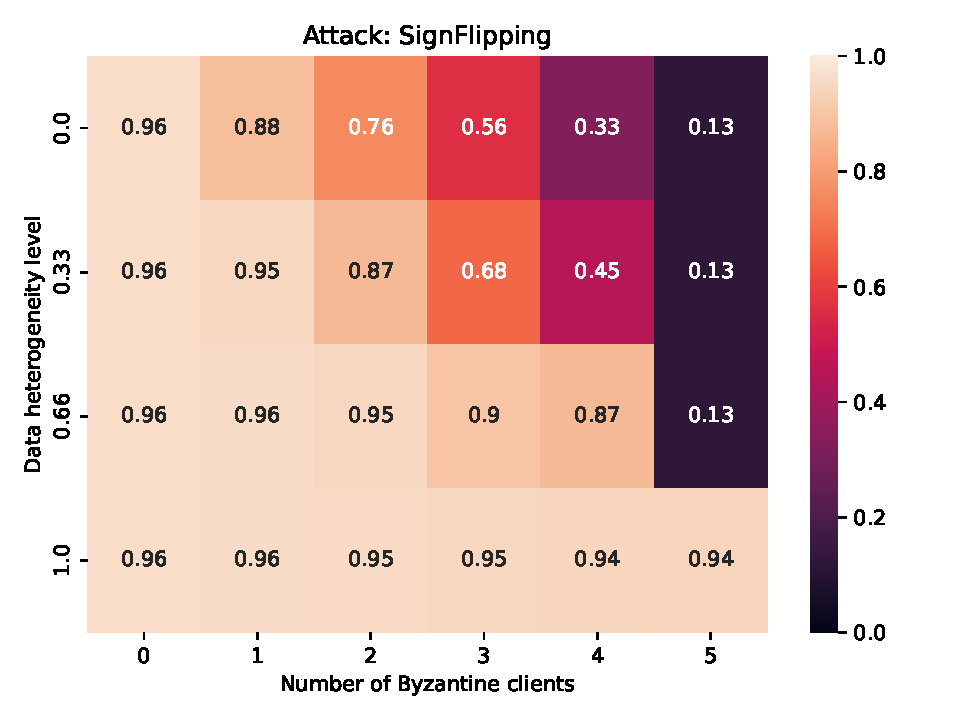
\includegraphics[width=\textwidth]{../plots/robust_new_atan_sweep/alpha_1.0/test_SignFlipping_mnist_cnn_mnist_snn_gamma_similarity_niid_NNM_ARC_TrMean_nb_honest_clients_10_tolerated_f_equal_real.pdf}
        \caption{$\alpha = 1.0$}
        \label{fig:tm_sf_alpha_1_0}
    \end{subfigure}
    \vspace{0.2cm}
    \begin{subfigure}[b]{0.24\textwidth}
        \centering
        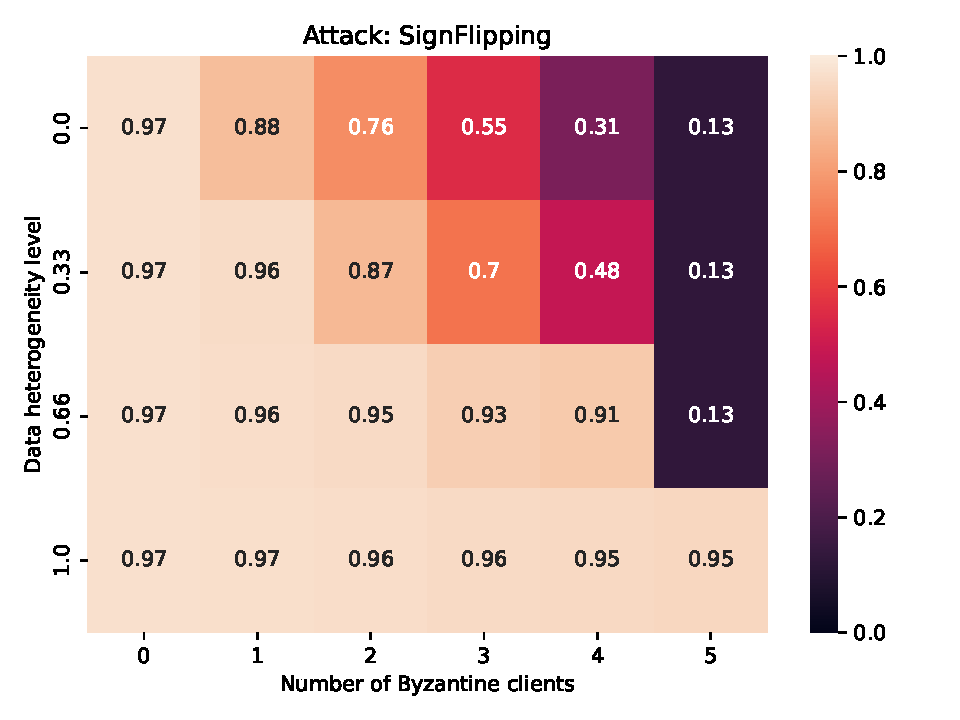
\includegraphics[width=\textwidth]{../plots/robust_new_atan_sweep/alpha_1.2/test_SignFlipping_mnist_cnn_mnist_snn_gamma_similarity_niid_NNM_ARC_TrMean_nb_honest_clients_10_tolerated_f_equal_real.pdf}
        \caption{$\alpha = 1.2$}
        \label{fig:tm_sf_alpha_1_2}
    \end{subfigure}
    \hfill
    \begin{subfigure}[b]{0.24\textwidth}
        \centering
        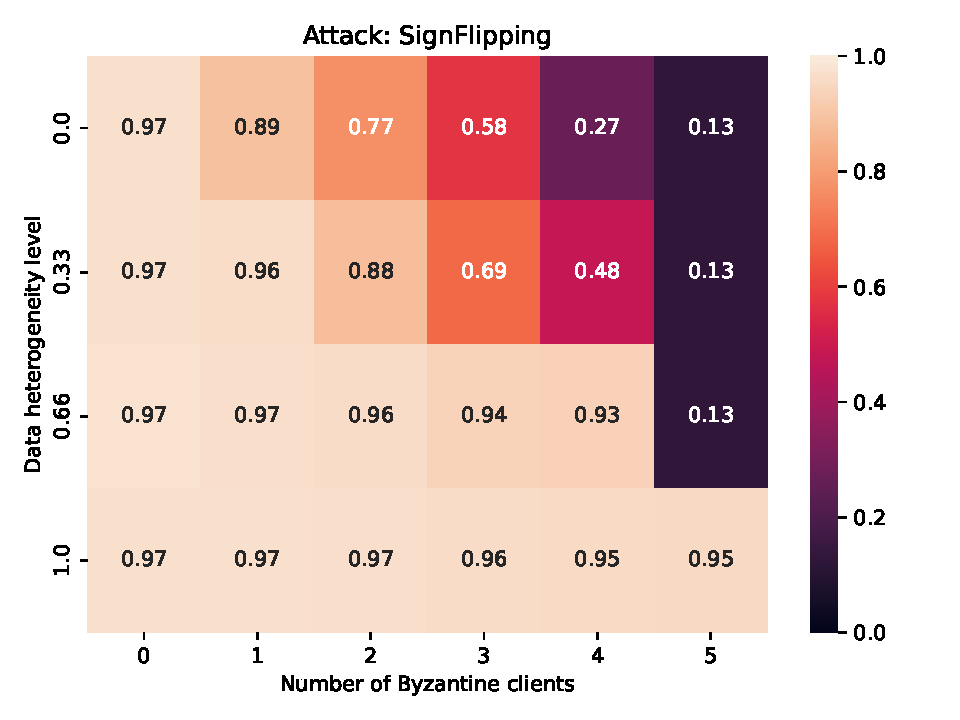
\includegraphics[width=\textwidth]{../plots/robust_new_atan_sweep/alpha_1.4/test_SignFlipping_mnist_cnn_mnist_snn_gamma_similarity_niid_NNM_ARC_TrMean_nb_honest_clients_10_tolerated_f_equal_real.pdf}
        \caption{$\alpha = 1.4$}
        \label{fig:tm_sf_alpha_1_4}
    \end{subfigure}
    \hfill
    \begin{subfigure}[b]{0.24\textwidth}
        \centering
        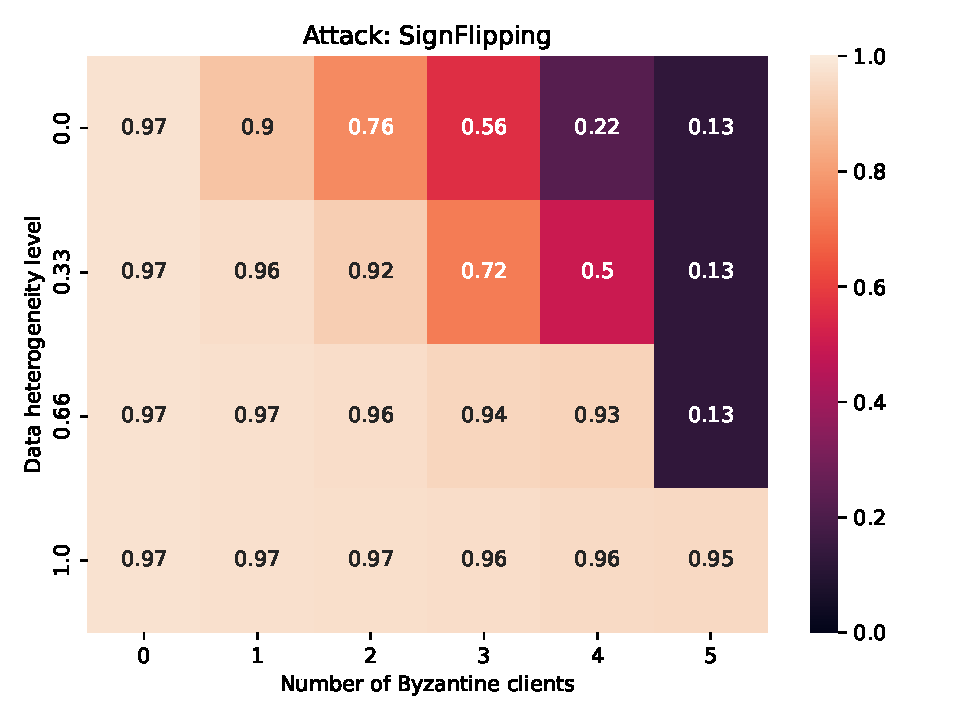
\includegraphics[width=\textwidth]{../plots/robust_new_atan_sweep/alpha_1.5/test_SignFlipping_mnist_cnn_mnist_snn_gamma_similarity_niid_NNM_ARC_TrMean_nb_honest_clients_10_tolerated_f_equal_real.pdf}
        \caption{$\alpha = 1.5$}
        \label{fig:tm_sf_alpha_1_5}
    \end{subfigure}
    \hfill
    \begin{subfigure}[b]{0.24\textwidth}
        \centering
        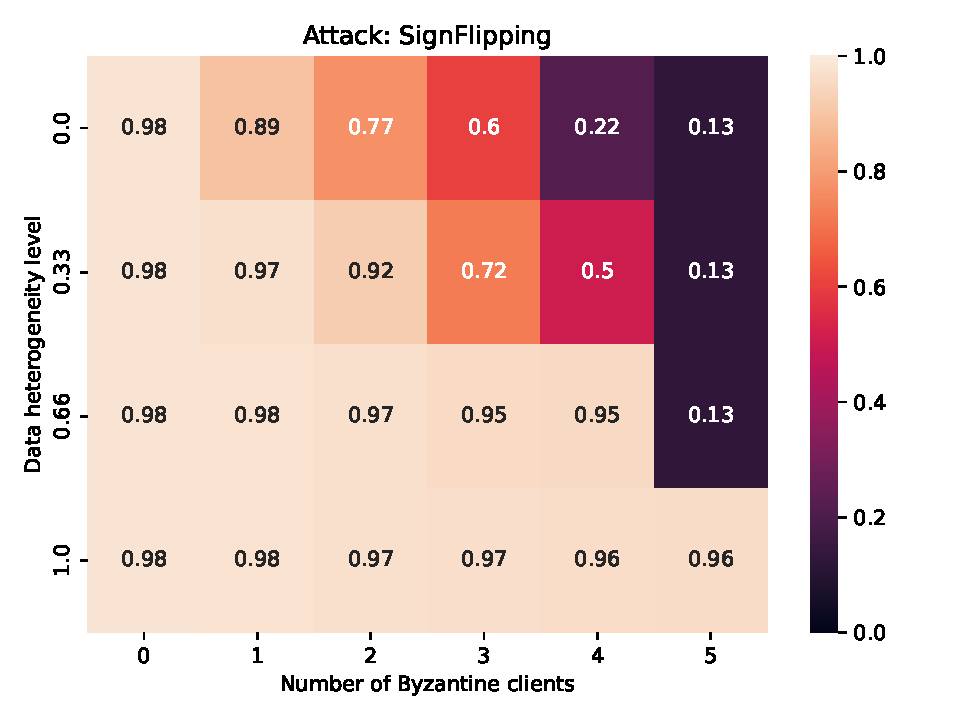
\includegraphics[width=\textwidth]{../plots/robust_new_atan_sweep/alpha_2.0/test_SignFlipping_mnist_cnn_mnist_snn_gamma_similarity_niid_NNM_ARC_TrMean_nb_honest_clients_10_tolerated_f_equal_real.pdf}
        \caption{$\alpha = 2.0$}
        \label{fig:tm_sf_alpha_2_0}
    \end{subfigure}
    \caption{Trimmed Mean performance under Sign Flipping across $\alpha$ values.}
    \label{fig:tm_sf_grid}
\end{figure}\clearpage
\subsubsection{TM under Optimal Inner Product Manipulation Attack}
\begin{figure}[htbp]
    \centering
    \begin{subfigure}[b]{0.24\textwidth}
        \centering
        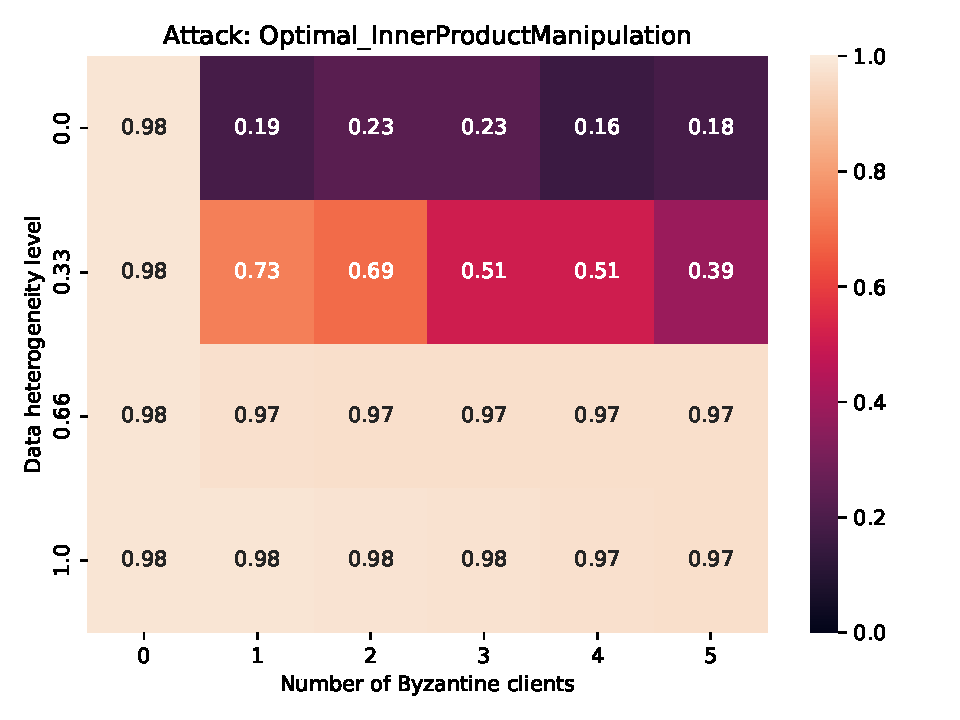
\includegraphics[width=\textwidth]{../plots/robust_comparison_sweep/test_Optimal_InnerProductManipulation_mnist_cnn_mnist_gamma_similarity_niid_NNM_ARC_TrMean_nb_honest_clients_10_tolerated_f_equal_real.pdf}
        \caption{CNN Baseline}
        \label{fig:tm_ipm_cnn}
    \end{subfigure}
    \hfill
    \begin{subfigure}[b]{0.24\textwidth}
        \centering
        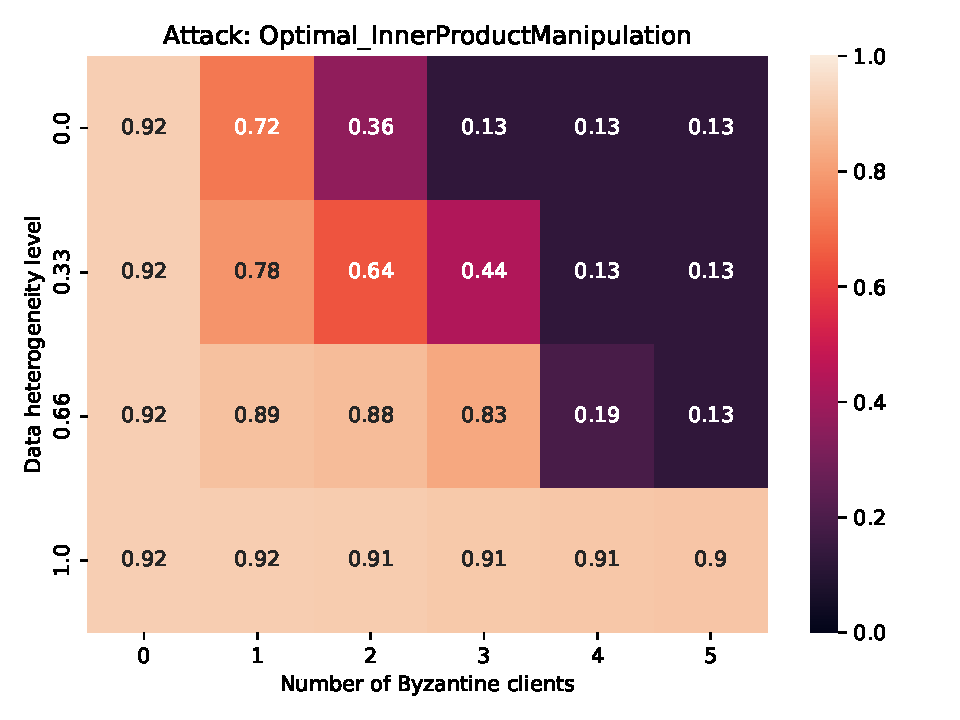
\includegraphics[width=\textwidth]{../plots/robust_new_atan_sweep/alpha_0.5/test_Optimal_InnerProductManipulation_mnist_cnn_mnist_snn_gamma_similarity_niid_NNM_ARC_TrMean_nb_honest_clients_10_tolerated_f_equal_real.pdf}
        \caption{$\alpha = 0.5$}
        \label{fig:tm_ipm_alpha_0_5}
    \end{subfigure}
    \hfill
    \begin{subfigure}[b]{0.24\textwidth}
        \centering
        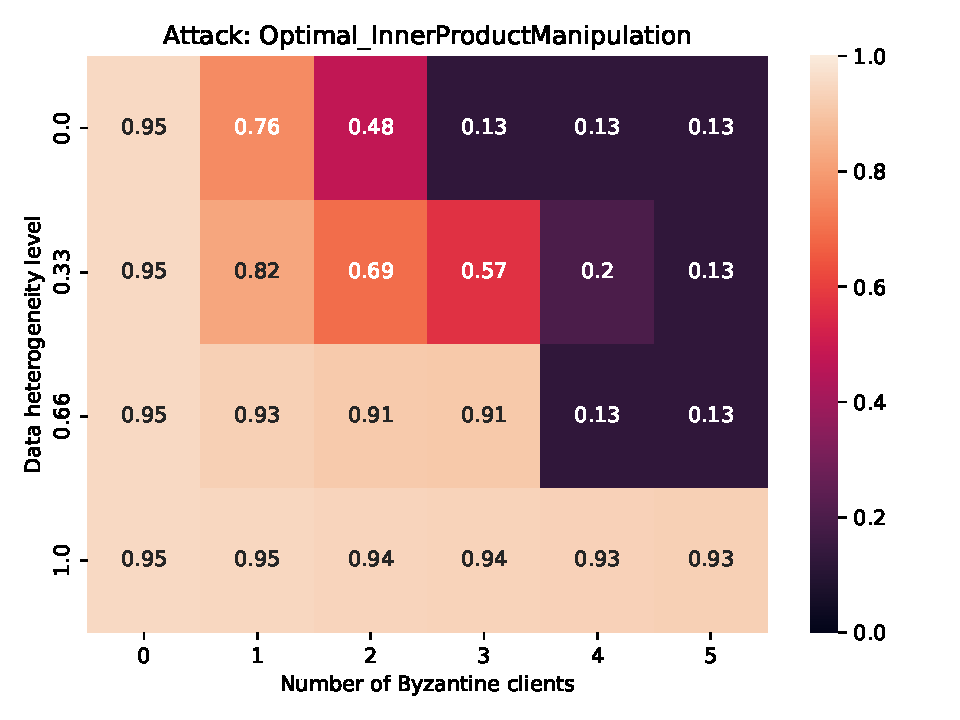
\includegraphics[width=\textwidth]{../plots/robust_new_atan_sweep/alpha_0.75/test_Optimal_InnerProductManipulation_mnist_cnn_mnist_snn_gamma_similarity_niid_NNM_ARC_TrMean_nb_honest_clients_10_tolerated_f_equal_real.pdf}
        \caption{$\alpha = 0.75$}
        \label{fig:tm_ipm_alpha_0_75}
    \end{subfigure}
    \hfill
    \begin{subfigure}[b]{0.24\textwidth}
        \centering
        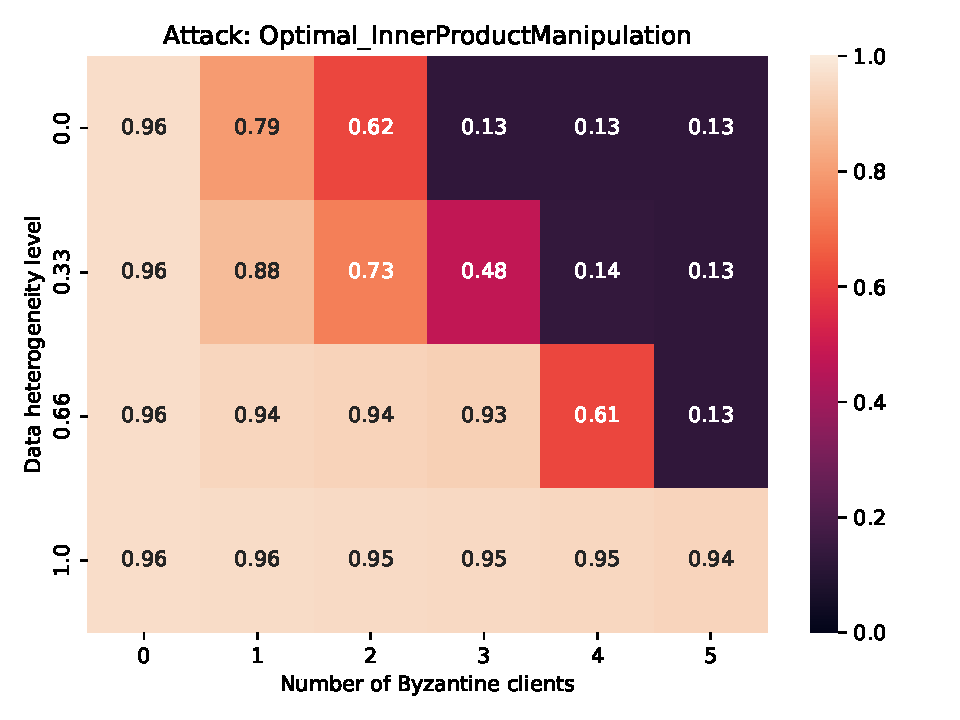
\includegraphics[width=\textwidth]{../plots/robust_new_atan_sweep/alpha_1.0/test_Optimal_InnerProductManipulation_mnist_cnn_mnist_snn_gamma_similarity_niid_NNM_ARC_TrMean_nb_honest_clients_10_tolerated_f_equal_real.pdf}
        \caption{$\alpha = 1.0$}
        \label{fig:tm_ipm_alpha_1_0}
    \end{subfigure}
    \vspace{0.2cm}
    \begin{subfigure}[b]{0.24\textwidth}
        \centering
        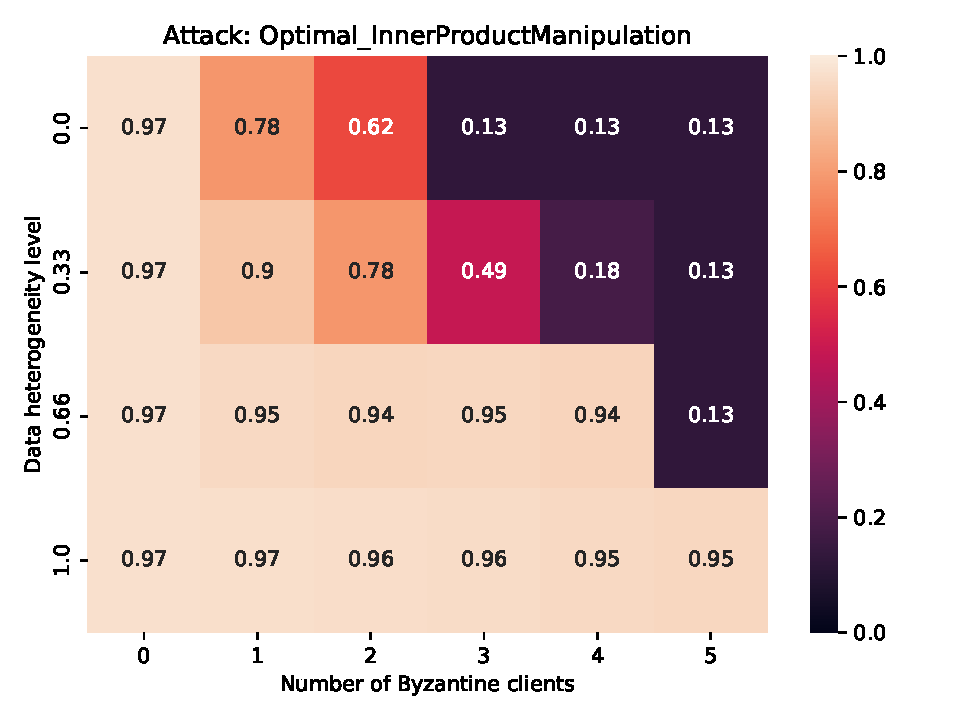
\includegraphics[width=\textwidth]{../plots/robust_new_atan_sweep/alpha_1.2/test_Optimal_InnerProductManipulation_mnist_cnn_mnist_snn_gamma_similarity_niid_NNM_ARC_TrMean_nb_honest_clients_10_tolerated_f_equal_real.pdf}
        \caption{$\alpha = 1.2$}
        \label{fig:tm_ipm_alpha_1_2}
    \end{subfigure}
    \hfill
    \begin{subfigure}[b]{0.24\textwidth}
        \centering
        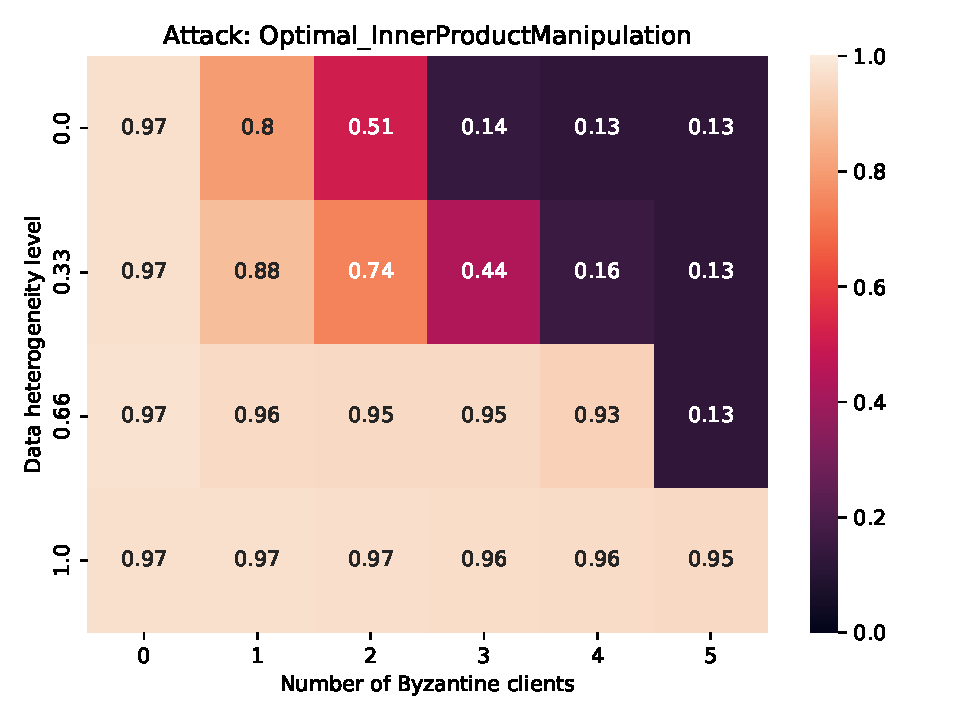
\includegraphics[width=\textwidth]{../plots/robust_new_atan_sweep/alpha_1.4/test_Optimal_InnerProductManipulation_mnist_cnn_mnist_snn_gamma_similarity_niid_NNM_ARC_TrMean_nb_honest_clients_10_tolerated_f_equal_real.pdf}
        \caption{$\alpha = 1.4$}
        \label{fig:tm_ipm_alpha_1_4}
    \end{subfigure}
    \hfill
    \begin{subfigure}[b]{0.24\textwidth}
        \centering
        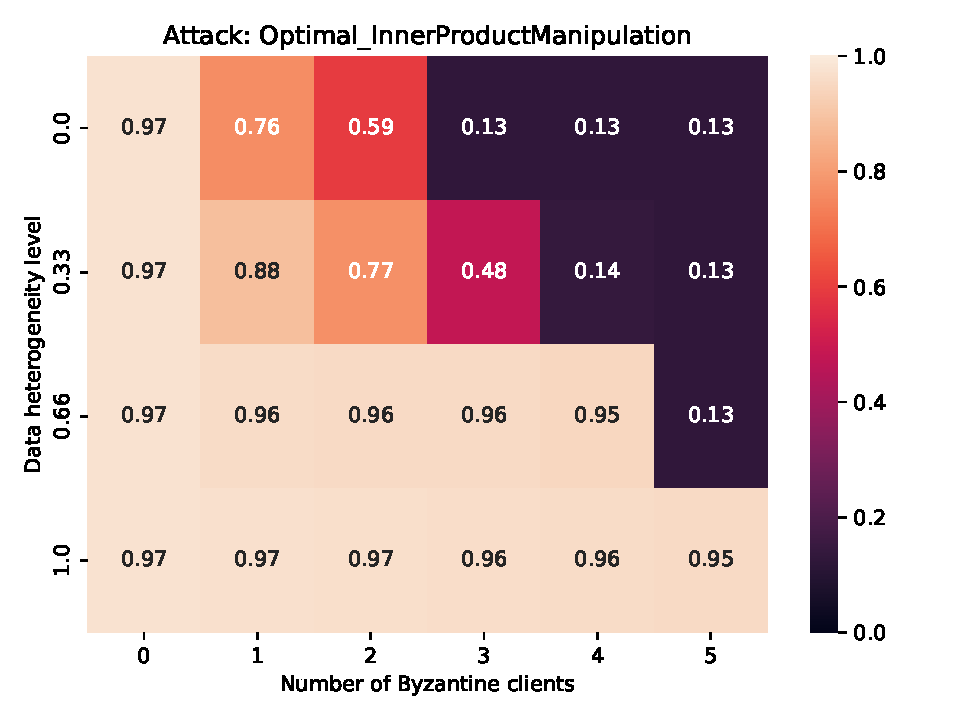
\includegraphics[width=\textwidth]{../plots/robust_new_atan_sweep/alpha_1.5/test_Optimal_InnerProductManipulation_mnist_cnn_mnist_snn_gamma_similarity_niid_NNM_ARC_TrMean_nb_honest_clients_10_tolerated_f_equal_real.pdf}
        \caption{$\alpha = 1.5$}
        \label{fig:tm_ipm_alpha_1_5}
    \end{subfigure}
    \hfill
    \begin{subfigure}[b]{0.24\textwidth}
        \centering
        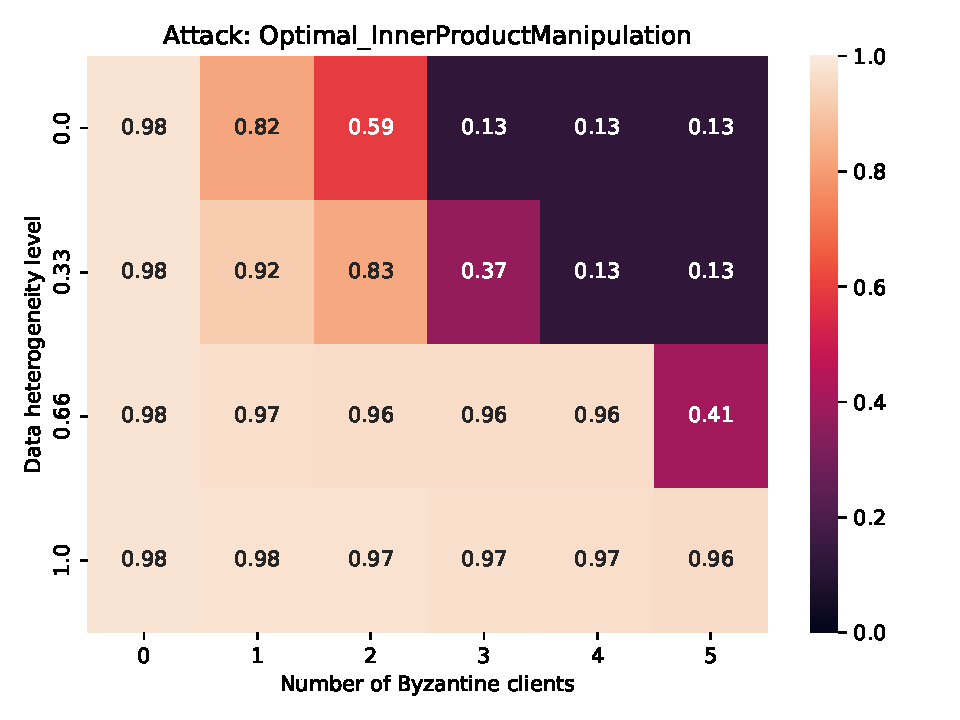
\includegraphics[width=\textwidth]{../plots/robust_new_atan_sweep/alpha_2.0/test_Optimal_InnerProductManipulation_mnist_cnn_mnist_snn_gamma_similarity_niid_NNM_ARC_TrMean_nb_honest_clients_10_tolerated_f_equal_real.pdf}
        \caption{$\alpha = 2.0$}
        \label{fig:tm_ipm_alpha_2_0}
    \end{subfigure}
    \caption{Trimmed Mean performance under Optimal Inner Product Manipulation across $\alpha$ values.}
    \label{fig:tm_ipm_grid}
\end{figure}
\end{document}
